\documentclass[a4paper]{report}
\usepackage[english]{babel}
\usepackage[utf8]{inputenc}
\usepackage{amsmath}
\usepackage{amsthm}
\usepackage{amsfonts}
\usepackage{amssymb}
\usepackage{natbib}
\usepackage{algorithm}
\usepackage{algorithmic}
\usepackage{mathtools}
\usepackage{epstopdf}
\usepackage{float}
\usepackage{url}
\usepackage{array,ragged2e}
\usepackage{xcolor}
\usepackage{listings}
\usepackage{mcode}

\newcolumntype{C}[1]{>{\Centering}m{#1}}

\newcommand{\R}{\mathbb{R}}
\newcommand{\N}{\mathbb{N}}
\newcommand{\Z}{\mathbb{Z}}
\newcommand{\C}{\mathbb{C}}
\newcommand{\dx}{\, \mathrm{d}}
\newcommand{\de}{\partial}
\newcommand {\argmin} {\mathop{\mathrm{argmin}}\limits}
\newcommand {\minimize} {\mathop{\mathrm{minimize}}\limits}
\newtheorem{theorem}{Theorem}[chapter]
\newtheorem{algoritmo}{Algorithm}
\newtheorem{defi}{Definition}[chapter]
\renewcommand{\qedsymbol}{$\lozenge$}

\setlength\parindent{0pt}
\setlength{\parskip}{6pt} %%distanza fra i paragrafi

\begin{document}

\begin{titlepage}
\begin{center}

% Upper part of the page

\textsc{\LARGE Universit\`{a} degli Studi di Ferrara}\\[1cm]

\textsc{Facolt\`{a} di Scienze Matematiche, Fisiche e Naturali}\\
\textsc{Corso di Laurea in Matematica, indirizzo Matematica Applicata}\\[1.5cm]


\includegraphics[width=4cm]{unife}\\[1cm]

% Title
\Large \textbf{Total Variation image denoising from Poisson data: Split Bregman and Alternating Extragradient methods} \\[0.5cm]


\vfill

% Author and supervisor
\begin{minipage}{0.4\textwidth}
\begin{flushleft} \large
\emph{Laureando:}\\
Davide Taviani \\
~
\end{flushleft}
\end{minipage}
\begin{minipage}{0.4\textwidth}
\begin{flushright} \large
\emph{Relatore:} \\
Chiar.ma Prof.ssa \\
Valeria Ruggiero
\end{flushright}
\end{minipage}

\vspace{3cm}

% Bottom of the page
{\large Anno Accademico 2010-2011}

\end{center}

\end{titlepage} 

\clearpage

\pagenumbering{Roman}

\setcounter{page}{1}
\tableofcontents
\pagebreak

\pagenumbering{arabic}

Nell'ambito multidisciplinare dell'elaborazione delle immagini, un problema di rilievo \`{e} costituito dalla individuazione delle tecniche numeriche per rimuovere il fenomeno chiamato rumore o \emph{noise}, ossia per ricostruire immagini degradate da effetti a carattere aleatorio. Questo problema \`{e} anche noto con il nome di \emph{denoising}.

Il tipo di \emph{noise} che ha avuto pi\`{u} attenzione in letteratura \`{e} quello di lettura, cio\`{e} dovuto all'amplificazione, da parte di un sistema elettronico, del segnale in uscita dal sistema di sensori, che trasformano i segnali da analogici a digitali. Per questo rumore, di tipo additivo, il modello pi\`{u} accreditato \`{e} quello di una distribuzione Gaussiana.

Un altro tipo di \emph{noise} \`{e} quello fotonico, che trae origine dalle fluttuazioni nel numero di fotoni che arrivano sul rivelatore, e che pu\`{o} essere descritto statisticamente attraverso una distribuzione multivariata di Poisson.

In alcuni casi, come ad esempio nella radiografia digitale, nella tomografia ad emissione, nella microscopia confocale a fluorescenza e nell'astronomia con telescopi ottici o a infrarossi, il rumore fotonico \`{e} prevalente su quello additivo. Questo fatto porta alla necessit\`{a} di generalizzare l'approccio usato per eliminare il rumore Gaussiano al rumore Poissoniano, riconducendo il problema alla minimizzazione di una funzione convessa, fortemente non lineare, nel suo dominio.

Nel caso dei regolarizzatori che preservano i bordi, come per il funzionale di \emph{Total Variation}, poich\'{e} la funzione \`{e} anche non differenziabile, viene introdotto un grado di ulteriore complessit\`{a} nella ricerca di un metodo numerico efficiente per la risoluzione del problema.

Scopo della tesi \`{e} descrivere il problema di denoising di immagini degradate da rumore Poissoniano e analizzare dal punto di vista teorico e numerico i metodi che rappresentano lo stato dell'arte per regolarizzazione con la funzione \emph{Total Variation}.

Nel primo capitolo si descrive il processo di formazione delle immagini, evidenziando l'origine delle varie perturbazioni che possono degradarle. Particolare attenzione si \`{e} data alla differenziazione fra le caratteristiche del rumore di tipo Gaussiano e quello di tipo Poissoniano.  Si \`{e} inoltre mostrato come il problema di ricostruzione di immagini sia un problema inverso mal posto nel senso di Hadamard, e quindi potenzialmente di difficile risoluzione; per questo motivo, nell'ambito della teoria Bayesiana, \`{e} stato mostrato come l'approccio di massima verosimiglianza e le tecniche di regolarizzazione consentano di ricondurre il problema alla soluzione di un problema di minimo vincolato.

Nel secondo capitolo sono stati analizzati dal punto di vista teorico i metodi di tipo Bregman e Split Bregman, mettendo in evidenza gli aspetti implementativi in termini di complessit\`{a} computazionale. Tali metodi possono essere ricondotti al metodo alle direzioni alternate dei moltiplicatori, ma possono essere interpretati anche come l'algoritmo di Douglas-Rachford, un particolare metodo \emph{proximal point}, applicato alla formulazione duale del problema di minimo. Dai noti risultati teorici su questi metodi, \`{e} possibile ricavare la convergenza dei metodi PIDAL e PIDSplit+, due metodi Split Bregman appositamente progettati per ricostruire dati affetti da rumore Poissoniano con regolarizzazione data dalla \emph{Total Variation}.

Nel terzo capitolo viene esaminata la formulazione primale-duale del problema di minimo, che porta a risolvere un problema di sella per una funzione convessa-concava. Esprimendo il problema variazionale come una particolare disequazione variazionale monotona su un dominio esprimibile come prodotto cartesiano dei domini delle variabili primale e duale, si \`{e} considerata la classe dei metodi extragradiente, adattando tale approccio al problema in esame.

In particolare viene descritto il metodo AEM, in cui ogni passo esegue una serie di aggiornamenti successivi di tipo Gauss-Seidel delle variabili primale e duale mediante opportuni passi di gradiente proiettato.

Nel quarto capitolo vengono infine svolte alcune simulazioni numeriche, sia considerando problemi test simulati, ovvero problemi per i quali si ha a disposizione l'immagine priva di rumore, che problemi reali. Per la prima classe di questi problemi test sono stati studiati e confrontati il metodo AEM e il metodo PID-
Split+, sia in termini di accuratezza che di efficienza numerica. Particolare enfasi \`{e} stata data all'analisi della velocit\`{a} di convergenza, sia per quanto riguarda le prime iterazioni, che rispetto al comportamento asintotico.

Per quanto riguarda i problemi di tipo reale, invece,  \`{e} stato dapprima stimato il parametro di regolarizzazione, usando sia il principio di discrepanza, recentemente enunciato in \citep{discr_princ}, che analizzando il comportamento delle soluzioni ottenute.

Sulla base dei valori ottenuti per il parametro di regolarizzazione, sono stati confrontati i metodi PIDSplit+ e AEM, sperimentando un criterio di arresto automatico. L'analisi sperimentale ha messo in evidenza un'ottima efficienza del metodo PIDSplit+ per opportune scelte di un parametro del metodo, che deve essere stimato dall'utente. D'altro canto, il metodo AEM ha messo in evidenza un buon comportamento, sia dal punto di vista dell'efficienza che dell'accuratezza dei risultati ottenuti, senza avere la necessit\`{a} di stimare alcun parametro, poich\'{e} la lunghezza del passo da cui dipende ogni iterazione \`{e} calcolata adattivamente.

In Appendice A, sono state incluse le definizioni di alcune matrici frequenti nei problemi di elaborazioni di immagini, come le matrici di Toepliz e quelle circolanti, mettendo in evidenza come le operazioni di base con queste matrici possano essere realizzate mediante la Trasformata Discreta di Fourier, efficientemente calcolabile con l'algoritmo Trasformata Veloce di Fourier. Inoltre, sono stati riportati in sintesi i principali risultati teorici sull'ottimizzazione vincolata (condizioni necessarie e sufficienti del primo e secondo ordine) e alcune importanti propriet\`{a} delle funzioni
convesse e monotone.

Nell'Appendice B, infine, sono stati allegati i codici MATLAB usati. 
\chapter{Image restoration} \label{chap1}

Image restoration is one of the most important topics in imaging science. To better understand that, this chapter will cover the principles behind image formation and errors that occur during this process.

\section{The image acquisition}

Images are acquired via an image system which consists in a optical part and a detector; they both have to be taken into account for an accurate modeling of the imaging process.

\subsubsection{The optical system}

The optical system can be summarized as a device which collects the light coming from an object to form a image in a plane, hence called the \emph{image plane}.

Since most imaging systems are exactly, or at least approximately, isoplanatic, if the light emitted by the object is spatially incoherent, then the following integral describes the linear relationship between the intensity of the object $x(s)$ and that of the image obtained $\tilde{f}(s)$:

\begin{align} \label{1.1}
\tilde{f}(s) = \int H(s-s')\, x(s') \dx s'
\end{align}

$H$ is called the \emph{impulse response}.

The expression can also be viewed as

$$\tilde{f}(s) = (H*x)(s)$$

where $*$ denotes the \emph{convolution} operator.

In case of a point light source in $s_0$, usually expressed with a Dirac $\delta$ function centered in $s_0$, under the hypothesis that the overall energy is conserved, its integral is costant at 1.

Thus, we have that $x(s) = \delta(s-s_0)$ and \eqref{1.1} can be rewritten as:

$$\tilde{f}(s) = H(s-s_0)$$

Then the impulse response coincides with the image obtained in case of point light sources. For this reason $H$ is also known as \emph{point spread function} (PSF). The PSF has also a practical meaning, since it represents the error due to the optical system known as \emph{blurring} (see Section \eqref{sec:blurring}).

In general, we will suppose the PSF to satisfy:

\begin{enumerate}
\item $H(s) \geq 0$
\item $\int H(s) \dx s = 1$
\end{enumerate}

\subsubsection{Detection}

Along with the optical part, the image system is characterized by another fundamental device, the \textbf{detector}, which is located in the image plane and measures the incoming radiation, converting it to electrical signals.

Some example of such detectors are the CCD (\emph{Charged Coupled Device}), often used in astronomy, APS (\emph{Active Pixel Sensor}), which is the most common sensor found in cell phone cameras and DSLRs cameras, and APD (\emph{Avalanche Photo-Diode}), one of the most important for fluorescence microscopy.

The detection process introduces the concept of \textbf{sampling}, which is a process performed on a uniform grid in the image plane: since it is impossible to store continuous informations, the image is stored as an array of pixels or voxels (depending on the dimension of the problem), and for this reason the equation \eqref{1.1} must be somehow discretized; thanks to the mapping provided by geometric optics, the image can be subdivided into pixels (or voxels), so that the convolution equation \eqref{1.1} is replaced by the matrix equation

\begin{align}
\label{1.2} \tilde{f}=Hx
\end{align}

The discrete convolution can assume different forms, depending on the boundary values: if we assume to have 0 in the boundaries, then the matrix $H$ is a block-Toepliz with Toepliz blocks (BTTP) matrix\footnote{See Section \ref{app:matrices} for a brief overview of such particular matrix structures.}, besides, if we assume the boundaries to be periodic (i.e. the first line is replicated as the $(n+1)$-th line, and similarly for every border), the matrix is a block-circulant with circulant blocks (BCCB) matrix\footnotemark[\value{footnote}].

The discrete PSF is  normalized to 1: $H^T e= e$, where $e$ denotes an array with all entries equal to 1.

Constraints due to the physical properties of the object can be imposed: a natural constraint is $x_i \geq 0$, $\forall i$.

Furthermore, every entry of $H$ is nonnegative and $He > 0$ (every row and every column of $H$ has at least a nonzero element).

\section{Errors in the image formation}

In the digital signal obtained by the image system, some errors can come at play; in general, the ones which are due to the radiation emitted by the object $x$ itself, the \emph{blurring} and \emph{noise}, are dominant.

\subsection{Blurring} \label{sec:blurring}

Blur is an error in the image which occurs during the acquisition, and, mathematically speaking, is connected to backward diffusion processes (such as the inversion of the heat equation), which are notoriously unstable.

In general, blur, along with its origin, can be divided into three main categories, each one with its own PSF:

\begin{itemize}
\item \emph{optical blur}, also often called ``out-of-focus blur'', which is due to the deviation of the image plane from the focus of an optical lens;
\item \emph{mechanical blur}, or ``motion blur'', which arises from the rapid mechanical motion of either the target object or image devices during the image acquisition process;
\item \emph{medium-induced blur} which is due to the scattering or optical turbulence of the media through which light rays travel.
\end{itemize}

The last one affects heavily astronomy and microscopy: for example, spatiotemporal variation of the physical properties of the atmosphere (such as temperature and density) could result in a randomly fluctuating distributions of the index of refraction, causing ``optical turbulence''; meanwhile, in microscopy, problems lie in the inhomogeneities in the refractive index of the specimen considered, which lead to a similar effect.

\subsection{Noise}

Noise can be roughly described as an \emph{unwanted} component of the image which is intrinsic to any image system.

There are several kind of noise: some occur naturally, some are induced by sensors, and others are a result from various processes like quantization, transmission of the informations and speckles in coherent light situations.

If the noise is \emph{additive}, a generic model for such process is:

$$f = \tilde{f} + n$$

where $\tilde{f}$ denotes the ideal image as in \eqref{1.1}, $n$ is the noise, and $f$ the real, noise-affected, observation.

The various noises generally considered are random in nature and therefore their exact values are random variables, which are best described using probabilistic notions.

While there are several image noise models, two of them are the most common in literature: Gaussian and Poisson Noise.

\subsubsection{Gaussian noise}

Gaussian noise is probably the most frequently occurring noise and for this reason it has been extensively studied.

Gaussian noise retains the properties of Gaussian distribution, and the Central Limit Theorem (CLT) is certainly one of the most important: it states that, given a large number of independent (or nearly so) variables, which are individually negligible compared to the sum, then the distribution of the sum of such variables has a Gaussian distribution. The theorem holds even if the individual random variables do not have a Gaussian distribution themselves or even the same distribution at all.

For this property, Gaussian noise is widely used to model thermal noise, which is due to the thermal agitation of charge carriers, usally electrons, inside a conductor, since the vibration of each electron can be seen as a random variable that fulfills the hypotesis of the CLT.

Gaussian noise, in addition, can be seen as the limit behavior of other noises with a different distribution, such as the \emph{photon noise} previously described.

The density function of univariate Gaussian noise, with mean $\mu$ and variance $\sigma^2$ is

$$p (x) = \frac{1}{\sqrt{2 \pi \sigma^2}}\, e^{-\frac{(x-\mu)^2}{2\sigma^2}}$$

with $-\infty < x < \infty$.

\subsubsection{Poisson noise}

In all imaging processes where images are obtained by means of the count of particles (photons in general) arriving in the image domain, the noise (also known as \emph{photon noise} or \emph{shot noise}) can be modeled with a Poisson distribution, meaning that the probability of receiving $k$ particles in a given interval of time $T$ is given by:

\begin{align}
p(k) = \dfrac{ e^{-\lambda} \lambda^k }{k!} \qquad \qquad k = 0,1,2, ...
\end{align}

where $\lambda$, proportional to $T$, is the expected value of the occurrencies.

If $N$ is the average number of photons collected, the \emph{signal-to-noise ratio} is $\sqrt{N}$; this explains why photon noise becomes more important when the number of photons collected is small, e.g. in low light conditions.

This statistical model is appropriate to describe data acquired in fluorescence microscopy, emission tomography, optical/infrared astronomy, and so on; even if in all these fields the wavelength of the photons is different, the statistics of the data remains the same, while the image system varies. Namely, the $H$ matrix in the equation \eqref{1.2} is a sparse matrix in tomography, and a convolution matrix in microscopy and in astronomy.

As a result of recent development and attention gained by medical application such as PET (\emph{Positron Emission Tomography}) and SPECT (\emph{Single Photon Emission Computerized Tomography}), major advances have been made and then transferred to other fields in which data are affected by Poisson noise.

A minor contribution to the noise can come from a phenomenon known as \emph{background emission}: in astronomy, for example, this emission is due to the sky, while in fluorescence microscopy the auto-fluorescence of both the medium and the sample along with the reflections of the excitation light must be taken into account. This background emission is again a random variable with Poisson distribution and an estimate of its expected value $b_i$ can be obtained by a preprocessing of the detected image. There are some cases in which the background value can be even larger than the signal itself; these images are called \emph{background dominated} and are an important challenge in astronomy.

In general, when the object and the background emission are statistically independent (or it can be reasonably assumed), their overall contribution is a Poisson random variable with the expected value $(Hx+b)_i$.

\section{Image restoration as an ill-posed inverse problem}

If we consider the problem of image restoration to be independent to sensor effects and without inherent noise, we have the equation \eqref{1.1}; in this case the problem is to determine the original object distribution $x$, given the recorded image $\tilde{f}$ and some knowledge about the PSF $H$.

A common method to do so is to employ operathor theory: given spaces of functions in which $x$ and $\tilde{f}$ are defined, considering the operator $T$:

$$T\{x\} \to \tilde{f}$$

we have that

$$T\{x\} = \int H(s-s')x(s') \dx s'$$

The problem of image restoration is then to find the inverse transformation $T^{-1}$ such that

$$T^{-1}\{\tilde{f}\} \to x$$

For this reason, most of the problems found in image processing are \textbf{inverse problems}.

A problem stands a ``good'' chance of solution by computation, using a stable algorithm, if it is \textbf{well posed} and \textbf{well-conditioned}.

A problem is well-posed in the sense of Hadamard if:

\begin{itemize}
\item a solution exists
\item the solution is unique
\item the solution depends continuously on the data, in some reasonable topology
\end{itemize}

Problems for which $T^{-1}$ does not exist, are said to be \emph{singular}. Even if such inverse operator exists, is unique and depends continuously on the data, it may be \emph{ill-conditioned}, i.e. a trivial perturbation in $\tilde{f}$ may result in nontrivial perturbations in $x$.

In particular, mathematically speaking, there exists an $\epsilon$, arbitrarily small, such that:

$$T^{-1} \{\tilde{f}+\epsilon\} = x + \delta$$

where $\delta \gg \epsilon$. If this is the case, $\delta$ is not arbitrarily small and therefore not negligible.

Summarizing, an ill-posed problem is one in which the inverse transformation may not have a solution or inherent data perturbations, such as noise, may result in undesirable effects in the solution by inverse transformation (\emph{ill-conditioning}).

The ill-posedness of image restoration can be proved by means of Riemann-Lebesgue lemma \citep{hunt}, which, applied to our case, states that:

$$\lim_{\alpha \to \infty} \int H(s-s') \sin(\alpha s') \dx s' = 0$$

Then

\begin{align}
\label{riem-leb}
\lim_{\alpha \to \infty} \int H(s-s') [x(s') + \sin(\alpha s')] \dx s' = \int H(s-s') x(s') \dx s' = \tilde{y}
\end{align}

In other words, a sinusoid of infinite frequency can be added to the object distribution $x$ and the result is identical to the image distribution $\tilde{y}$.  Then the image restoration problem is an ill-posed problem.

A direct implication of \eqref{riem-leb} is that we choose a small value $\epsilon_1$, there exist a value $A$ such that

$$\int H(s-s') \sin(\alpha s') \dx s' < \epsilon_1 \qquad \forall \alpha \geq A$$

Therefore

$$ \int H(s-s')[x(s') + sin(\alpha s')] \dx s' = \tilde{y} + \epsilon\qquad \forall \alpha \geq A,\; |\epsilon| < \epsilon_1$$

This shows that if an infinitesimally small value $\epsilon$ is chosen and added to the image distribution $\tilde{y}$, this cannot be separate, in the sense of image restoration, from an original object distribution that has an additional component of a sinusoid with frequency $\alpha$. Since $\epsilon$ can be arbitrarily small, a trivial perturbation cannot be distinguished from a finite, nontrivial perturbation in the original object distribution. Then, also the solution of the inverse transformation is ill-conditioned.

\section{Regularization}

As seen before, image restoration is an ill-posed problem and the key to a successful solution of this kind of problems lies in its regularization: assuming the image is affected by noise with a known statistical distribution, we will adopt the Bayesian framework proposed by Geman and Geman \citep{bayes}, which consist in the use of additional \emph{a priori} informations about both the clean signal $\tilde{y}$ and the noise, along with their statistical properties.

Then the computation of the \emph{maximum a posteriori} estimate is reduced to the minimization of the negative-log of the posterior probability density.

\subsection{Likelihood}

Using the previous notation, let $f$ denote the detected signal (an array of integer nonnegative numbers, which represent the number of photons detected) with elements $f_i$ ($i \in S$, which will be implied from this moment on, can be either a single or multiple index, depending on the nature of the problem).

In case of Gaussian noise, $f$ is the realization of a random variable $F$; its elements $F_i$ are Gaussian random variables with mean $(Hx+b)_i$ and variance $\sigma_i$.

Assuming the random variables associated with each pixel are statistically independent, then the probability distribution of $F$, for given $H$, $x$ and $b$, is:

\begin{align}
\label{g_like}
p_F(f;x) = \prod_{i \in S} \dfrac{1}{\sqrt{2\pi\sigma_i^2}} e^{-\frac{(f_i-(Hx+b)_i)^2}{2\sigma_i^2}}
\end{align}

In case of Poisson noise, on the other side, $f$ is the realization of a Poisson random variable $f$ (with elements $F_i$) with the expected value $Hx+b$. Assuming again that the random variables associated with each pixel are statistically independent, then the probability distribution of $F$, for given $H$, $x$ and $b$, is:

\begin{align}
\label{p_like}
p_F(f;x) = \prod_{i \in S} \dfrac{e^{-(Hx+b)_i} (Hx+b)_i^{f_i}}{f_i!}
\end{align}

The \emph{maximum likelihood} (ML) approach consists substantially in the addition of a function of $x$, the \emph{likelihood}, defined by $L_f^F(x) = p_F(f;x)$, where $f$ is the given detected image. Then a ML estimate is any maximizer of such function.

In case of Gaussian noise, if we take the negative logarithm, the equation \eqref{g_like} is reduced to:

$$\phi_0(x) = \sum_{i \in S} \left\{ \log{\dfrac{1}{\sqrt{2\pi\sigma_i^2}}}+\dfrac{(f_i-(Hx+b)_i)^2}{2\sigma_i^2} \right\}$$

Since $\log{\dfrac{1}{\sqrt{2\pi\sigma_i^2}}}$ is costant, the minimization of such equations is essentially the weighed least square approximation:

\begin{align}
\label{weigh_lsq}
\min \dfrac{1}{2} \left| \left| \dfrac{f_i-(Hx+b)_i}{\sigma_i}\right| \right|_2^2
\end{align}

Considering Poisson noise, however, taking the negative logarithm and using the Stirling formula ($\log f_i! \simeq -f_i + f_i \log f_i$), the equation \eqref{p_like} is reduced to:

\begin{align}
\label{KL}
\phi_0(x) = \sum_{i \in S} \left\{f_i \log{\frac{f_i}{(Hx+b)_i}}+(Hx+b)_i - f_i\right\}
\end{align}

where we assume $f_i \log f_i =0$ if $f_i =0$.

This function is called the generalized  Kullback-Leibler (KL) divergence (also known as Csisz\`{a}r I divergence) of $x$ from $f$, and its minimization is reduced on the nonnegative orthant, since is well-known to be convex, nonnegative and coercive on the nonnegative orthant, so that minimizers exist and are global.

If the equation $Hx+b = y$ has a nonnegative solution $x^*$, this is also a minimizer of the KL function, since we have

$$\phi_0(x^*) = \sum_{i \in S} \left\{ f_i \log{\dfrac{f_i}{f_i}} + f_i - f_i \right\} = 0$$

In general, because of the extreme ill-conditioning of $H$, a solution could be difficult to compute. Furthermore, $f$ is degraded by noise. Consequently, a minimizer of $\phi_0(x)$ may not provide a sensible solution of the image deblurring problem.

For this reason it is necessary to ``regularize'' the maximum likelihood approach by a suitable \emph{prior}, which describes the known statistical properties of the unknown solution.

\subsection{The Bayesian Approach}
\label{bayesian_framework}

In the Bayesian approach, the unkown object $x$ is also considered as a realization of a multi-valued random variable, and the \emph{a priori} information is encoded into the given probability distribution $p_X(x)$ of this random variable, the so-called \emph{prior}.

If the probability distribution \eqref{p_like} is viewed as a conditional probability of $F$ for a given value of $x$, i.e. $p_F (f;x) = p_F (f|X=x)  =: p_F(f|x)$, then the Bayes formula (hence the name) states:

$$p_X(x|f) = \dfrac{p_F(f|x)p_X(x)}{p_F(x)}$$

If in this equation we insert the detected value of $f$, we obtain the \emph{posterior probability distribution} of $X$,

$$P_f^X(x) = L_f^F(x)\dfrac{p_X(x)}{p_F(f)}$$

As for the choice of the prior, in general it is assumed that $X$ is either a Gibbs random field or a Markov random field (MRF). Thanks to Hammersley-Clifford Theorem, however, any MRF is equivalent to a suitable Gibbs random field, so we will focus on that.

The Gibbs random field is a random variable with a probability distribution given by

$$p_X(x) = \dfrac{1}{Z} e^{-\beta \phi_1(x)}$$

where $\phi_1(x)$ is a given function, usually called energy function or \textbf{penalty function}, and $Z$ is a normalization constant.

By definition, the \emph{maximum a posteriori} (MAP) estimate is any maximizer of the posterior probability distribution; if we take again the negative logarithm of this function, we can see that a MAP estimate is any $x_\beta^*$ which minimizes

\begin{align}
\label{map}
\phi(x) = \phi_0 (x)+ \beta \phi_1 (x)
\end{align}

where $\beta$ is the so-called \emph{regularization parameter}.

Functions of the form of \eqref{map} have been used in several applications, with different form of the penalizing function $\phi_1(x)$.

\begin{align}
\label{defTV}
\begin{aligned}
&\mbox{Quadratic Penalization} && \phi_1(x) = \dfrac{||x||_2^2}{2} \\
&\mbox{Quadratic Laplacian} && \phi_1(x) = \dfrac{||\Delta x||_2^2}{2} \\
&\mbox{Total Variation (TV)} && \phi_1(x) = \sum_{i \in S} ||(\nabla x)_i||_2
\end{aligned}
\end{align}

where $(\nabla x)_i$ is the discrete approximation of the gradient at $x_i$.

Different criteria have been proposed for the choice of the regularization parameter $\beta$: in case of Gaussian noise, to solve the weighed least squares problem \eqref{weigh_lsq}, a good principle is the so-called \emph{Mozorov discrepancy principle}\citep{mozorov}. Considering Poisson noise, however, a possible way, proposed in \citep{discr_princ}, is to find the value of $\beta$ such that

\begin{align}
\label{discr}
D_{KL} (Hx_\beta^*+b,f) = \dfrac{n}{2}
\end{align}

where $D_{KL}$ is the same as \eqref{KL}, and $n$ is the cardinality of $S$.

\section{Formulation of the problem}

In this work, we will focus on the image denoising from data corrupted by Poisson noise; the PSF is then the identity matrix ($H=I$) and, if we suppose that there is no \emph{background emission}, the KL divergence \eqref{KL} can be rewritten as:

$$\phi_0(x) = \sum_{i \in S} \left\{f_i \log{\dfrac{f_i}{x_i}} + x_i - f_i \right\}$$

A minimizer $x^*$ for such functional is $x^* = f$, which means that the solution is the detected image itself. Since we know that $f$ is a noisy image, $f$ cannot be a feasible solution for our problem; we overcome this with a penalty function $\phi_1(x)$ (see \eqref{map}).

The domain of the resulting functional $\phi(x) = \phi_0(x)  + \beta \phi_1(x) $ is

\begin{align}
\label{domain}
X = \left\{ \begin{array}{ll}
x \geq \eta > 0&f_i > 0 \\
x \geq 0&f_i=0
\end{array}\right.
\end{align}

where

$$\eta = \min \{ f_i | f_i > 0 \} $$

Such function $\phi(x)$ is convex and coercive and thus the solution of the problem

\begin{align}
\label{ROF}
\min_{x \in X} \phi(x)
\end{align}

is unique\footnote{See Section \ref{app:convex} for a brief overview on the properties of convex functionals.}.

The gradient and Hessian of the $\phi_0$ are given by:

\begin{align*}
\nabla \phi_0 (x) &= 1 - \dfrac{f}{x} \\
\nabla^2 \phi_0 (x) &= diag\left(\dfrac{f}{x^2}\right)
\end{align*}

where the quotient is defined in the Hadamard sense, i.e. pixel by pixel (or voxel by voxel).

We will consider $\phi_1(x)$ as the TV functional as in \eqref{defTV}. It is important to note that such function is not always differentiable. Such TV functional was has been introduced in \citep{rof}. The function \eqref{ROF}, with $\phi_0(x) = \dfrac{1}{2}||x-y||_2^2$ is also known as ROF model.

In the following chapters, for the TV functional we will use expression

\begin{align}
\phi_1(x) = \sum_{i=1}^n ||A_i x||_2
\end{align}

where $n = s \times t$ is the number of pixels of the image, and $A_i$ (for $i=1,...,n$) is a $2 \times n$ matrix with null entries except for

\begin{align*}
a_{1,i} = -1 && a_{1,i+1} = 1 \\
a_{2,i} = -1 && a_{1,i+t+1} = 1
\end{align*}

where the pixels in the image are ordered column-wise.

In addition, for further reference, we consider the matrix $A$ as the $2n \times n$ matrix defined by

\begin{align} \label{matrixA}
A = \begin{pmatrix}
A_1 \\
\vdots \\
A_n
\end{pmatrix}
\end{align} 
\chapter{Bregman Iterations and Split Bregman methods}

\section{Bregman Iterations}

In this section, we will introduce the Bregman Iteration and show that it can be used to solve a wide variety of constrained optimization problems.

Then we will introduce the ``Split Bregman methods", which we will apply to TV functional for image denoising.

\subsection{Subgradient and subdifferential}

\begin{defi}
Let $E: U \to \R$ be a real-valued function (not necessarily convex) defined on a convex open set in the Euclidean space $\R^n$: a vector $v$ in that space is called a \textbf{subgradient} \citep{rockafellar} at a point $x_0 \in U$ if for any $x \in U$ one has:

$$E(x) - E(x_0) \geq v^T(x-x_0)$$

\end{defi}

The set of all subgradients at $x_0$ is called the \textbf{subdifferential} at $x_0$ and is denoted $\de E(x_0)$. The subdifferential is always a convex closed set and if $f$ is convex and finite near $x_0$, it is nonempty.

The subgradient gives an affine global underestimator of $E(x)$. If $E(x)$ is convex, it has at least one subgradient at every internal point of the domain. Furthermore, if $E(x)$ is convex and differentiable, the gradient vector $\nabla E(x_0)$ is a subgradient of $E(x)$ at $x_0$.

\begin{theorem}
Let $E: U \to \R$ be a convex function, $U \subset R^n$.

$x_0 \in U $ is a global minimum $ \iff 0 \in \de E(x_0)$
\end{theorem}
\begin{proof}

\begin{align*}
x_0 \mbox{ is a global minimum } &\iff E(x) \geq E(x_0) \qquad \forall x \in U \\
&\iff E(x)-E(x_0) \geq 0 \\
&\iff E(x)-E(x_0) \geq 0^T (x-x_0) \\
&\iff 0 \in \de E(x_0)
\end{align*}
\end{proof}

\subsection{Bregman distance}

\begin{defi}
The Bregman distance \citep{reg_tv} associated with a convex function $E$ at the point $v$ is

\begin{align}
D^p_E (u,v) = E(u) - E(v) - p^T(u-v)
\end{align}

where $p$ is the subgradient of $E$ at $v$.
\end{defi}

If $E(u)$ is strictly convex, $D^p_E(u,v)$ is also strictly convex in $u$ for each $v$, and as a consequence $D^p_E(u,v)=0$ if and only if $u=v$.

However, even for a continuously differentiable and strictly convex function, the Bregman distance is not a distance in the usual sense, since in general $D^p_E(u,v) \neq D^p_E(v,u)$, and the triangle inequality does not hold.

It is, however, a measure of closeness in the sense that $D^p_E(u,v) \geq 0$, and $D^p_E(u,v) \geq D^p_E(w,v)$ for $w$ on the line segment between $u$ and $v$.

\section{Bregman iteration for unconstrained minimization problem}

Let us consider two non-negative energy functionals, $E$ and $H$. We assume that $H$ is differentiable and such that

$$\min_{x \in \R^n} H(x) = 0$$

and $E$ is not everywhere differentiable.

We consider the following problem:

\begin{align} \label{minimized_problem}
\min_x \left\{ E(x) + \lambda H(x) \right\}
\end{align}

where $\lambda$ is a positive number.

We can modify this problem, iteratively solving:

\begin{align} \label{breg_iter}
\begin{aligned}
 x^{(k+1)} &= \argmin_x \left\{ D^p_E \left(x,x^{(k)}\right) + \lambda H(x) \right\} \\
 &= \argmin_x \left\{ E(x) - {p^{(k)}}^T \left(x-x^{(k)}\right) + \lambda H(x) \right\}
 \end{aligned}
 \end{align}

We have $0 \in \de\left(\left(D^p_E\left(x,x^{(k)}\right)+\lambda H)(x^{(k+1)}\right)\right)$; if $p^{(k+1)} \in \de E\left(x^{(k+1)}\right)$, we have that

\begin{align}
 p^{(k+1)} = p^{(k)} - \lambda \nabla H \left(x^{(k+1)}\right)
 \end{align}

To simplify, if we denote $q^{(k+1)} = \lambda \nabla H\left(x^{(k+1)}\right)$, we have $p^{(k+1)} + q^{(k+1)} = p^{(k)}$.

Then, if we put $p^{(0)} = 0$, we have:

\begin{align} \label{pk}
\begin{aligned}
p^{(1)} &= p^{(0)} - q^{(1)} = -q^{(1)} \\
p^{(2)} &= p^{(1)} - q^{(2)} = -q^{(1)} -q^{(2)} \\
&\vdots \\
p^{(k+1)} &= - \sum_{j=1}^{k+1} q^{(j)}
\end{aligned}
\end{align}

In \citep{reg_tv} the authors analyze the convergence of this Bregman iterative scheme, and it is shown that under fairly weak assumption on $E$ e $H$, we have that

\begin{align} \label{breg_cvg}
\lim_{k \to \infty} H\left(x^{(k)}\right) = 0
\end{align}

\begin{theorem}
Assume that $E$ and $H$ are convex functionals, and that $H$ is differentiable. We also assume that solutions to the sub-problems in \eqref{breg_iter} exist. We then have:

\begin{enumerate}
\item $H\left(x^{(k+1)}\right) \leq H\left(x^{(k)}\right)$ for every $k$.
\item if $x^*$ is a minimizer of $H(x)$ such that $E(x^*)<\infty$, then
$$H\left(x^{(k)}\right) \leq H(x^*) + \dfrac{E(x^*)}{\lambda k}$$

and in particular $\{ x^{(k)} \}$ is a minimizing sequence.

This sequence has converging subsequences to a minimizer $x^*$ of $H(x)$. If such minimizer is unique, $x^{(k)} \to x^*$ as $k \to \infty$.
\end{enumerate}
 \end{theorem}
 \begin{proof}
 See \citep{reg_tv}, Proposition 3.2 and Theorem 3.3.
 \end{proof}

Note that $x^*$ is not a solution of problem \eqref{minimized_problem}.

\section{Bregman iteration for constrained minimization problem} \label{sec:unconstrained}

We assume that we have to solve the following problem

\begin{align} \label{minimized_2}
\min_x E(x) \qquad \qquad \mbox{such that} \qquad Ax=b
\end{align}

We put $H(x) = Ax-b$, for some linear operator $A$ and vector $b$. We want to apply the formula \eqref{minimized_problem}, so we make this into an uncostrained problem, using a quadratic penalty function, thus having

\begin{align}
\min_x \left\{ E(x) + \dfrac{\lambda}{2} ||Ax-b||^2_2 \right\}
\end{align}

The Bregman iteration for this problem is

\begin{align}
&\begin{aligned} \label{breg_iter2}
x^{(k+1)} &= \argmin_x \left\{ D^p_E \left(x,x^{(k)}\right) + \dfrac{\lambda}{2} ||Ax-b||^2_2 \right\} \\
 &= \argmin_x \left\{ E(x) - {p^{(k)}}^T\left(x-x^{(k)}\right) + \dfrac{\lambda}{2} ||Ax-b||^2_2 \right\}
\end{aligned}  \\
\notag \\
&p^{(k+1)} = p^{(k)} - \lambda A^T (Ax^{(k+1)} - b)
\end{align}

In this case, since $H(x) = Ax-b$, $H$ is linear with respect to $x$, and we have

\begin{align}
q^{(k)} = \lambda \nabla H\left(x^{(k)}\right) = \lambda A^T \left(Ax^{(k)}-b\right) \label{qk}
\end{align}

From \eqref{pk} and \eqref{qk},  we have $p^{(k+1)} \in \mbox{ range}(A^T)$.

If $p^{(0)}=0, x^{(0)}=0$ and we put $p^{(k)} = \lambda A^T \left(b^{(k)}-b\right)$, with $b^{(0)} = b$, we have

\begin{align*}
p^{(k+1)} &=  p^{(k)} - \lambda A^T(Ax^{(k+1)}-b) \\
\\
\lambda A^T (b^{(k+1)}-b) &= \lambda A^T \left(b^{(k)}-b\right) -\lambda A^T (Ax^{(k+1)} - b) \\
\\
\lambda A^T b^{(k+1)} - \lambda A^T b &= \lambda A^T b^{(k)} - \lambda A^T b - \lambda A^T A x^{(k+1)} + \lambda A^T b \\
\\
\lambda A^T b^{(k+1)} &= \lambda A^T b^{(k)} - \lambda A^T A x^{(k+1)} + \lambda A^T b \\
\\
\lambda A^T b^{(k+1)} &= \lambda A^T \left(b^{(k)} - Ax^{(k+1)} + b\right)
\end{align*}

Then

\begin{align} \label{alg1-2}
b^{(k+1)} = b^{(k)} + b - Ax^{(k+1)}
\end{align}

In \eqref{breg_iter2} we have:

\begin{align*}
-{p^{(k)}}^T \left(x-x^{(k)}\right) + \dfrac{\lambda}{2} ||Ax-b||_2^2 &= {p^{(k)}}^T \left(x^{(k)}-x\right) + \dfrac{\lambda}{2} ||Ax-b||_2^2 \\
 &= \lambda \left(b^{(k)}-b\right)^T \left(Ax^{(k)}-Ax\right) +  \dfrac{\lambda}{2} ||Ax-b||_2^2
\end{align*}

Moving on to the gradient we have:

\begin{align*}
\nabla \left(\lambda \left(b^{(k)}-b\right)^T \left(Ax^{(k)}-Ax\right) +  \dfrac{\lambda}{2} ||Ax-b||_2^2 \right) &= -\lambda A^T \left(b^{(k)}-b\right) + 2 \dfrac{\lambda}{2} A^T (Ax-b) \\
 &= \lambda A^T \left(b-b^{(k)}\right) +  \lambda A^T (Ax-b) \\
 &= \lambda A^T \left(Ax-b+b-b^{(k)}\right) \\
 &= \lambda A^T \left(Ax-b^{(k)}\right) \\
 &= \nabla \left(\dfrac{\lambda}{2} \left|\left|Ax-b^{(k)}\right|\right|_2^2 \right)
\end{align*}

Then the Bregman iteration can be written as

\begin{align}
\begin{aligned}
x^{(k+1)} &= \argmin_x \left\{ E(x) + \dfrac{\lambda}{2} \left|\left|Ax-b^{(k)}\right|\right|_2^2 \label{alg1-1} \right\} \\
\\
b^{(k+1)} &= b^{(k)} + b - Ax^{(k+1)}
\end{aligned}
\end{align}

Since $H(x) = Ax-b$, we have that \eqref{breg_cvg}  is now

\begin{align}\label{breg_cvg2}
\lim_{k \to \infty} Ax^{(k)} = b
\end{align}

where the convergence is in the 2-norm sense.

\begin{theorem} \label{th:1.2}
Let $E:\R^n \to \R$ be convex; let $A: \R^n \to \R^m$ be linear. Consider the algorithm \eqref{alg1-1} and suppose that some iterate $x^*$ satisfies $Ax^* = b$.

Then $x^*$ is a solution to the original constrained problem \eqref{minimized_2}.
\end{theorem}
\begin{proof}
Let $x^*$ and $b$ be such that $Ax^* = b$ and

\begin{align}
x^* = \argmin_x \left\{ E(x) + \dfrac{\lambda}{2}||Ax-b||_2^2 \right\} \label{theo1.2-1}
\end{align}

Let $\hat{x}$ be a true solution to \eqref{minimized_2}. Then $Ax^* = b = A\hat{x}$, which implies that

\begin{align}
||Ax^* - b ||_2^2 = ||A\hat{x}-b^*||_2^2 \label{theo1.2-2}
\end{align}

Because $x^*$ satisfies \eqref{theo1.2-1}, we have

\begin{align}
E(x^*) + \dfrac{\lambda}{2}||Ax^*-b||_2^2 \leq E(\hat{x}) + \dfrac{\lambda}{2}||A\hat{x}-b||_2^2 \label{theo1.2-3}
\end{align}

Finally, note that \eqref{theo1.2-2}-\eqref{theo1.2-3}) together imply:

$$E(x^*) \leq E(\hat{x})$$

Because $\hat{x}$ satisfies the original optimization problem, this inequality can be sharpened to an equality, showing that $x^*$ solves \eqref{minimized_2}.
\end{proof}

This theorem shows that, provided that the algorithm converges in the sense of \eqref{breg_cvg2}, the iterates $x^{(k)}$ will get arbitrarily close to a solution of the original constrained problem. Furthermore, the proof does not use the linearity of $A$.

There are some advantages with these Bregman iteration techniques over traditional penalty functions: first of all, Bregman iterations converge quickly when applied to certain types of functions, especially for problems where $E$ contains an L1- regularization term. The second advantage is that the value of $\lambda$ in \eqref{minimized_problem} is constant, and thus we can choose a good value for it, which minimizes the condition number of the sub-problems, also avoiding numerical instabilities that occur as $\lambda \to \infty$, that arise when using penalty methods.

\section{Split Bregman methods}

We will now solve

\begin{align} \label{prob:split}
\min_x \left\{|\Phi(x)|+H(x)\right\}
\end{align}

where $H$ and $|\Phi|$ are convex functionals, and $\Phi$ is differentiable. The key to our methods is to decouple the L1 and L2 portion of the energy in \eqref{prob:split}. We then consider the problem

\begin{align} \label{prob:split2}
\min_{x,d} \left\{ |d| + H(x) \right\} \qquad \qquad \mbox{ such that} \qquad d=\Phi(x)
\end{align}

which is clearly equivalent to the previous one. Then, we proceed to convert \eqref{prob:split2} to an unconstrained problem

\begin{align}
\min_{x,d} \left\{ |d| + H(x) + \dfrac{\lambda}{2} ||d-\Phi(x)||_2^2 \right\}
\end{align}

If we put $E(x,d) = |d| + H(x)$ and we define $A(x,d) = d-\Phi(x)$ we can see that  we have to solve the same problem as in Section \ref{sec:unconstrained}.

Then, the Bregman iteration is:

\begin{align} \label{breg_iter_split}
\begin{aligned}
\left(x^{(k+1)},d^{(k+1)} \right) &= \argmin_{x,d} \left\{ D^p_E \left(x,x^{(k)},d,d^{(k)}\right) + \dfrac{\lambda}{2} ||d-\Phi(x)||_2^2 \right\} \\
\\
&= \argmin_{x,d} \left\{ E(x,d) - {p_x^{(k)}}^T\left(x-x^{(k)}\right) + \right. \\
&\left. \qquad + {p_d^{(k)}}^T\left(x-x^{(k)}\right)  + \dfrac{\lambda}{2}||d-\Phi(x)||_2^2 \right\} \\
\\
p_x^{(k+1)} &= p_x^{(k)} - \lambda {\left(\nabla \Phi\left(x^{(k+1)}\right)\right)}^T\left(\Phi\left(x^{(k+1)}\right)-d^{(k+1)}\right) \\
\\
p_d^{(k+1)} &= p_d^{(k)} - \lambda \left(d^{(k+1)} - \Phi\left(x^{(k+1)}\right)\right)
\end{aligned}
 \end{align}

 After having applied the simplification \eqref{alg1-1}, we have the Bregman iteration:

 \begin{align}
  \label{alg2-1} \left(x^{(k+1)},d^{(k+1)}\right) &= \argmin_{x,d} \left\{ |d| + H(x) + \dfrac{\lambda}{2} \left|\left|d-\Phi(x)-b^{(k)}\right|\right|_2^2 \right\} \\
  \label{alg2-2} b^{(k+1)} &= b^{(k)} + \left(\Phi\left(x^{(k+1)}\right) - d^{(k+1)}\right)
 \end{align}

In this case we put
\begin{align*}
p_x^{(k+1)} &= \lambda \nabla \Phi\left(x^{(k+1)}\right)^T b^{(k+1)} \\
p_d^{(k+1)} &= \lambda b^{(k+1)}
\end{align*}

In order to implement this algorithm, we must be able to solve the problem \eqref{alg2-1}; having split the L1 and L2 components of this functional, we can perform this minimization efficiently, by iteratively minimizing with respect to $x$ and $d$ separately:

\begin{align}
\mbox{Step 1: }\qquad x^{(k+1)} &= \argmin_x \left\{H(x) + \dfrac{\lambda}{2} \left|\left|d^{(k)}-\Phi(x) - b^{(k)}\right|\right|_2^2 \right\} \label{split-1} \\
\mbox{Step 2: }\qquad  d^{(k+1)} &= \argmin_d \left\{|d| +  \dfrac{\lambda}{2} \left|\left| d - \Phi\left(x^{(k+1)}\right) - b^{(k)}\right|\right|_2^2 \right\} \label{split-2}
\end{align}

The scheme (\ref{split-1}-\ref{split-2}-\ref{alg2-2}) is known as \textbf{Split Bregman iteration} \citep{breg_l1}.

Having decoupled $x$ from the L1 portion of the problem, Step 1 is now differentiable. We can proceed by explicitly computing the optimal value of $d$ using the shrinkage operator:

\begin{align*}
d_j^{(k+1)} = shrink\left(\Phi(x)_j + b_j^{(k)}, \dfrac{1}{\lambda}\right)
\end{align*}

where the following operator solves $\argmin_d \left\{|d| + \dfrac{1}{2\gamma}||d-z||^2\right\}$

$$d =  shrink(x,\gamma) = \dfrac{z}{|z|} max(|z|-\gamma,0) $$

\subsection{Implementation of the Split Bregman iteration}

\begin{algorithm}[H]
\caption{Split Bregman iteration}
\begin{algorithmic}
\WHILE{$\left|\left|x^{(k)}-x^{(k+1)}\right|\right|_2 > tol$}
\STATE
\STATE $x^{(k+1)} = \argmin_x \left\{ H(x) + \frac{\lambda}{2} \left|\left|d^{(k)}-\Phi(x) - b^{(k)} \right|\right|_2^2 \right\}$
\STATE
\STATE $d^{(k+1)} = \argmin_d \left\{ |d| + \frac{\lambda}{2}\left|\left|d-\Phi\left(x^{(k+1)}\right)-b^{(k)}\right|\right|_2^2 \right\}$
\STATE
\STATE $b^{(k+1)} = b^{(k)}+\left(\Phi\left(x^{(k+1)}\right)-d^{(k+1)}\right)$
\STATE
\ENDWHILE
\end{algorithmic}
\end{algorithm}

Examining the Theorem \ref{th:1.2}, it is easy to observe that any fixed point of the split Bregman algorithm is a minimizer of the original problem \eqref{prob:split2}, even if the subproblem  \eqref{split-1} is inexactly solved.

Let $(x^*,d^*,b^*)$ be a fixed point of (\ref{alg2-1}-\ref{alg2-2}). The fixed point satisfies $b^* = b^* + \Phi(x^*) - d^*$, which implies that $d^* = \Phi (x^*)$. This result, combined with \eqref{alg2-1}, satisfies the condition of theorem \ref{th:1.2}, showing that $(x^*,d^*)$ is a solution of the constrained problem \eqref{prob:split2}.

In \citep{deblurring} and \citep{operator} the Bregman iteration is traced back to the \emph{augmented Lagrangian algorithm} discussed by Hestenes in \citep{hestenes}, and Powell in \citep{powell}, with the only difference that in the Bregman iteration the sequence $\{b^{(k)}\}$ is scaled by a factor $\lambda$. The convergence properties of the augmented Lagriangan algorithm are well known in literature, then the convergence of the Bregman iteration can be derived also from that of the augmented Lagrangian algorithm, see \citep{bertsekas}.

In \citep{deblurring} and \citep{operator} it is furthermore observed that the idea to minimize alternatingly with respect to the variables was presented also for the augmented Lagrangian methods in \citep{gabaymercier} \citep{glowinski}.

The resulting algorithm is called the \emph{alternating direction method of multipliers} \citep{gabay}, which is equivalent to the alternating split Bregman algorithm.

If we consider a dual formulation of the problem \eqref{prob:split}, it is possible to observe that the Bregman iteration is equivalent to the \emph{proximal point algorithm} of Rockafellar applied to the dual problem. Furthermore, the split Bregman methods coincides with the \emph{Douglas Rachford splitting method} applied to the dual problem, see \citep{Eckstein}.

Then the convergence properties of the Bregman iteration and of the split Bregman method can be deduced from that of the proximal point algorithm and of the Douglas Rachford splitting method respectively.

\section{TV denoising with split Bregman iteration}

TV denoising is considered to be one of the best denoising models for both Gaussian and Poisson noise, but also one of the hardest to compute.

In this section, we will show how the Split Bregman thechnique can be used to solve this kind of problems in a simple and extremely efficient way.

\subsection{Gaussian noise}
\subsubsection{Anisotropic model}

We begin by addressing this anisotropic problem:

\begin{align}
\label{an:prob} \min_x \left\{ |D_i x| + |D_j x| + \dfrac{\mu}{2} ||x-f||_2^2\right\}
\end{align}

where:

\begin{align*}
&D_i x\;\mbox{ is the column vector of the forward difference }\;x_{i+1,j}-x_{i,j}\\
&D_j x \;\mbox{ is the column vector of the forward difference }\;x_{i,j+1}-x_{i,j}
\end{align*}

With the notations of Chapter \ref{chap1}, $D_i$ and $D_j$ are matrices such that

$$PA = \begin{pmatrix} D_i \\
D_j \end{pmatrix}
$$

where $P$ is a $2n \times 2n$ permutation matrix that reorders the rows of $A$ \eqref{matrixA} by considering the odd rows first, and then the even rows.


To apply Bregman splitting, we first replace $D_i x$ by $d_i$ e $D_j x$ by $d_j$. Thus we have the constrained problem

\begin{align*}
\min_{x,d_i,d_j} \left\{ |d_i| + |d_j| + \dfrac{\mu}{2} ||x-f||_2^2\right\} \qquad \mbox{ such that } \; \; d_i = D_i x \; \; \mbox{ and } \; \; d_j = D_j x
\end{align*}

To weakly enforce the constraints, we add penalty function terms:

\begin{align*}
\min_{x,d_i,d_j} \left\{ |d_i| + |d_j| + \dfrac{\mu}{2} ||x-f||_2^2 + \dfrac{\lambda}{2} ||d_i - D_i x||_2^2 + \dfrac{\lambda}{2} ||d_j - D_j x||_2^2 \right\}
\end{align*}

Finally, we strictly enforce the constraints by applying the Bregman iteration \eqref{alg2-1}:

\begin{align*}
\min_{x,d_i,d_j} \left\{ |d_i| + |d_j| + \dfrac{\mu}{2} ||x-f||_2^2 + \dfrac{\lambda}{2} \left|\left|d_i - D_i x -b_i^{(k)}\right|\right|_2^2 + \dfrac{\lambda}{2} ||d_j - D_j x-b_j^{(k)}||_2^2 \right\}
\end{align*}

where the proper values of $b_i^{(k)}$ and $b_j^{(k)}$ are chosen through Bregman Iteration.

The resulting scheme is the following \citep{breg_l1}:

\begin{align*}
x^{(k+1)} &= \argmin_x \left\{ \dfrac{\mu}{2} ||x-f||_2^2|| + \dfrac{\lambda}{2} \left|\left|d_i^{(k)} - D_i x - b_i^{(k)}\right|\right|_2^2 + \dfrac{\lambda}{2} \left|\left|d_j^{(k)} - D_j x -b_j^{(k)}\right|\right|_2^2 \right\} \\
\\
d_i^{(k+1)} &= \argmin_{d_i} \left\{ |d_i| + \dfrac{\lambda}{2} \left|\left|d_i - D_i x^{(k+1)}-b_i^{(k)}\right|\right|_2^2 \right\} \\
\\
d_j^{(k+1)} &= \argmin_{d_j} \left\{ |d_j| + \dfrac{\lambda}{2} \left|\left|d_j - D_j x^{(k+1)}-b_j^{(k)}\right|\right|_2^2 \right\} \\
\\
b_i^{(k+1)} &= b_i^{(k)} + \left(D_i x^{(k+1)} - d_i^{(k+1)} \right) \\
\\
b_j^{(k+1)} &= b_j^{(k)} + \left(D_j x^{(k+1)} - d_j^{(k+1)} \right)
\end{align*}

The first subproblem has the following optimality condition:

\begin{align}
(\mu I - \lambda \Delta) x^{(k+1)} = \mu f + \lambda D_i^T \left(d_i^{(k)}-b_i^{(k)}\right) + \lambda D_i^T \left(d_j^{(k)}-b_j^{(k)}\right)
\end{align}

where $\Delta = - D_i^T D_i - D_j^T D_j$.

In order to achieve optimal efficiency, we wish to use a fast iterative algorithm to get approximate solutions to this system. Because the system is strictly diagonally dominant, the most natural choice is the Gauss-Seidel method, which, in this case, can be written component-wise as $x_{r,s}^{(k+1)} = G_{r,s}^{(k)}$, where

\begin{align*}
G_{r,s}^{(k)} &= \dfrac{\lambda}{\mu + 4 \lambda} \left(x_{r+1,s}+x_{r-1,s}+x_{r,s+1}+x_{r,s-1}+d_{i,r-1,s}-d_{i,r,s} + d_{j,r,s-1}^{(k)}\right.+ \\
&- \left.\,d_{j,r,s}^{(k)} - b_{i,r-1,s}^{(k)} + b_{i,r,s}^{(k)} - b_{j,r,s-1}^{(k)} + b_{j,r,s}^{(k)} \right) + \dfrac{\mu}{\mu + 4 \lambda}f_{r,s}
\end{align*}

In this case the value of $x_{.,.}$ are at the step $k$ or $k+1$ according to the order of solution.

Then, using this solver, we have the following algorithm:

\begin{algorithm}[H]
\caption{Split Bregman method for Anisotropic TV}
\begin{algorithmic}
\STATE $u^{(0)} = f$
\STATE
\STATE $d_i^{(0)} = d_j^{(0)} = b_i^{(0)} = b_j^{(0)}=0$
\STATE
\WHILE{ $\left|\left|x^{(k)}-x^{(k-1)}\right|\right|_2 > tol$}
\STATE
\STATE $x^{(k+1)} = G^{(k)}$
\STATE
\STATE $d_i^{(k+1)} = shrink \left(D_i x^{(k+1)} + b_i^{(k)},\dfrac{1}{\lambda}\right)$
\STATE
\STATE $d_j^{(k+1)} = shrink \left(D_j x^{(k+1)} + b_j^{(k)},\dfrac{1}{\lambda}\right)$
\STATE
\STATE $b_i^{(k+1)} = b_i^{(k)} + \left(D_i x^{(k+1)} - d_i^{(k+1)}\right)$
\STATE
\STATE $b_j^{(k+1)} = b_j^{(k)} + \left(D_j x^{(k+1)} - d_j^{(k+1)}\right)$
\ENDWHILE
\end{algorithmic}
\end{algorithm}

The split Bregman method has the advantage that before the convergence is reached, the intermediate images are smooth; most of the image noise is eliminated during the first 10 iterations.

\subsubsection{Isotropic model}

The split Bregman technique can be used also with the isotropic TV model with Gaussian noise: in this case we wish to solve

$$\min_x \left\{ \sum_r \sqrt{(D_i x)_r^2+(D_j x)_r^2} + \dfrac{\mu}{2}||x-f||_2^2 \right\}$$

Like we did before, we split the L1 and L2 components by setting $D_i x = d_i$ and $D_j x = d_j$.

The split Bregman formulation then becomes:

$$\min_{x,d_i,d_j} \left\{ ||(d_i,d_j)||_2 + \dfrac{\mu}{2} ||x-f||_2^2 \right\} \qquad \mbox{ such that } \; \; d_i = D_i x \; \; \mbox{ and } \; \; d_j = D_j x$$

where

$$||(d_i,d_j)||_2 = \sum_{r,s} \sqrt{d_{i,r,s}^2 + d_{j,r,s}^2}$$

Note that the $d_i$ and $d_j$, unlike in the anisotropic case, do not decouple. This changes the way in which these variables must be treated.

Enforcing the constraints as we did in the anisotropic case, adding penalty function terms and applying the Bregman iteration, we have:

$$\min_{d_i,d_j} \left\{ ||(d_i,d_j)||_2 + \dfrac{\mu}{2} ||x-f||_2^2 \dfrac{\lambda}{2} ||d_i - D_i x - b_i ||_2^2 + \dfrac{\lambda}{2} ||d_j - D_j x - b_j ||_2^2 \right\}$$

The resulting scheme is the following:

\begin{align*}
x^{(k+1)} &= \argmin_x \left\{ \frac{\mu}{2}||x-f||_2^2 + \frac{\lambda}{2}\left|\left|d_i^{(k)} - D_i x - b_i^{(k)}\right|\right|_2^2 + \right. \\
&\left. \qquad+\frac{\lambda}{2}\left|\left|d_j^{(k)} - D_j x - b_j^{(k)}\right|\right|_2^2 \right\} \\
\\
\left(d_i^{(k+1)},d_j^{(k+1)}\right) &= \argmin_{d_i,d_j} \left\{ \left|\left|(d_i,d_j)\right|\right|_2 + \frac{\lambda}{2} \left|\left|d_i - D_i x^{(k)} - b_i^{(k)} \right|\right|_2^2 + \right. \\
&\left. \qquad+\frac{\lambda}{2} \left|\left|d_j - D_j x^{(k)} - b_j^{(k)} \right|\right|_2^2 \right\} \\
\\
b_i^{(k+1)} &= b_i^{(k)} + \left(D_i x^{(k+1)} - d_i^{(k+1)}\right) \\
\\
b_j^{(k+1)} &= b_j^{(k)} + \left(D_j x^{(k+1)} - d_j^{(k+1)}\right)
\end{align*}

Despite the fact that $d_i$ and $d_j$ do not decouple as in the anisotropic case, we can still explicitly solve the minimization problem using a generalized shrinkage formula:

\begin{align*}
d_i^{(k+1)} &= \max \left(s^{(k)} - \dfrac{1}{\lambda},0\right) \dfrac{D_i x^{(k)} + b_i^{(k)}}{s^{(k)}} \\
d_j^{(k+1)} &= \max \left(s^{(k)} - \dfrac{1}{\lambda},0\right) \dfrac{D_j x^{(k)} + b_j^{(k)}}{s^{(k)}}
\end{align*}

where

\begin{align}
\label{iso:sk} s^{(k)} = \sqrt{\left(D_i x^{(k)} + b_i^{(k)}\right)^2 + \left(D_j x^{(k)} + b_j^{(k)}\right)^2}
\end{align}

If we apply once again the Bregman iteration to this problem, we get the minimization algorithm for the isotropic TV functional:

\begin{algorithm}[H]
\caption{Split Bregman method for Isotropic TV}
\begin{algorithmic}
\STATE $x^{(0)} = f$
\STATE
\STATE $d_i^{(0)} = d_j^{(0)} = b_i^{(0)} = b_j^{(0)}=0$
\STATE
\WHILE{ $\left|\left|x^{(k)}-u^{k-1}\right|\right|_2 > tol$}
\STATE
\STATE $x^{(k+1)} = G^{(k)}$
\STATE
\STATE $d_i^{(k+1)} = \max \left(s^{(k)} - \dfrac{1}{\lambda},0\right) \dfrac{D_i x^{(k)} + b_i^{(k)}}{s^{(k)}}$
\STATE
\STATE $d_j^{(k+1)} = \max \left(s^{(k)} - \dfrac{1}{\lambda},0\right) \dfrac{D_j x^{(k)} + b_j^{(k)}}{s^{(k)}}$
\STATE
\STATE $b_i^{(k+1)} = b_i^{(k)} + \left(D_i x^{(k+1)} - d_i^{(k+1)}\right)$
\STATE
\STATE $b_j^{(k+1)} = b_j^{(k)} + \left(D_j x^{(k+1)} - d_j^{(k+1)}\right)$
\ENDWHILE
\end{algorithmic}
\end{algorithm}

\subsection{Poisson noise}

We consider the following denoising problem for data affected by Poisson noise:

\begin{align}
\label{pidproblem}
\min_{x \in X} \left\{ \sum_{i=1}^n f_i \log{\dfrac{f_i}{x_i}}+x_i-f_i + \beta \sum_{i=1}^n ||A_i x||_2 \right\}
\end{align}

where $X$ is the same as defined in \eqref{domain} and $A$ is the matrix defined in \eqref{matrixA}. We will denote by $\Phi(Ax)$ the term $ \sum_{i=1}^n ||A_i x||_2$.

\subsubsection{PIDAL and PIDSplit+ algorithms}

In \citep{deblurring} the authors propose two different versions for the split Bregman iteration. In order to decouple the KL function and the TV, we begin by setting as constraints $w_1 = x$ and $w_2 = x$.

We then add to \eqref{pidproblem} the term $\dfrac{1}{2\gamma} ||x-w_1||_2^2 + \dfrac{1}{2\gamma} ||x-w_2^2||_2^2$

We have to minimize

$$ \sum_{i=1}^n f_i \log \dfrac{f_i}{(w_1)_i}+(w_1)_i - f_i + \beta \Phi(Aw_2) + \dfrac{1}{2\gamma} ||x-w_1||_2^2 + \dfrac{1}{2\gamma} ||x-w_2^2||_2^2 $$

The algorithm to solve this unconstrained problem is named PIDAL and it is stated as follows:

\begin{algorithm}[H]
\caption{PIDAL}
\begin{algorithmic}
\STATE $b_1^{(0)} = b_2^{(0)} = 0$
\STATE
\STATE $w_1^{(0)} = f$
\STATE
\STATE $w_2^{(0)} = f$
\STATE
\FOR{$k=1,...$ until a stopping criterion is reached}
\STATE
\STATE $x^{(k+1)} = \argmin_x \left\{ \left|\left|b_1^{(k)}+x-w_1^{(k)}\right|\right|_2^2 + \left|\left|b_2^{(k)}+x-w_2^{(k)}\right|\right|_2^2 \right\}$
\STATE
\STATE $w_1^{(k+1)} = \argmin_{w_1} \left\{ \displaystyle \sum_{i=1}^n \left( f_i \log \frac{f_i}{(w_1)_i} + (w_1)_i -f_i\right) + \right.$
\STATE $\left.\qquad\qquad + \dfrac{1}{2\gamma} \left|\left|b_1^{(k)} + x^{(k+1)} - w_1 \right|\right|_2^2 \right\}$
\STATE
\STATE $w_2^{(k+1)} = \argmin_{w_2} \left\{\beta \Phi(Aw_2) + \dfrac{1}{2\gamma}\left|\left|b_2^{(k)}+x^{(k+1)} - w_2\right|\right|_2^2\right\}$
\STATE
\STATE $b_1^{(k+1)} = b_1^{(k)} + x^{(k+1)} -w_1^{(k+1)}$
\STATE
\STATE $b_2^{(k+1)} = b_2^{(k)} + x^{(k+1)} -w_2^{(k+1)}$
\ENDFOR
\end{algorithmic}
\end{algorithm}

The first two steps can be solved explicitly:

\begin{align*}
x^{(k+1)} &= \left(\left(w_1^{(k)} -b_1^{(k)}\right) + \left(w_2^{(k)} -b_2^{(k)}\right) \right) / 2 \\
w_1^{(k+1)} &= \dfrac{1}{2} \left(b_1^{(k)} + x^{(k+1)} - \gamma + \sqrt{\left(b_1^{(k)} + x^{(k+1)}-\gamma\right)^2 + 4\gamma f} \right)
\end{align*}

For the third step we use a method for the denoising problem with Gaussian noise.

The PIDAL algorithm ensures that the sequence $w_1^{(k+1)}$ is nonnegative and it converges to a nonnegative image, but at every step we have to apply a Split Bregman Method (or another one) to determine $w_2^{(k+1)}$.

In order to simplify the approach, we introduce the indicator function: let $l_{x \geq \eta}$ denote the indicator function of $X$ defined as

$$ l_{x \geq \eta} (x) = \left \{ \begin{array}{ll}
0 & x \geq \eta \\
\infty & \mbox{ otherwise}\end{array} \right.
$$

We then apply the alternating split Bregman algorithm to:

\begin{align} \label{pidal}
\min_x \left\{ \sum_{i=1}^n x_i - f_i log(x_i) + \beta \Phi(Ax) + l_{x\geq \eta} \right\}
\end{align}

We can see this problem as the sum of three different functionals:

\begin{align*}
f_1(x) &:= \sum_{i=1}^n x_i - f_i log(x_i) \\
f_2(Ax) &:= \beta \Phi(Ax) \\
f_3(x) &:= l_{x\geq \eta}
\end{align*}

With this substitution we have now three constraints, $w_1 = x$, $w_2 = Ax$, $w_3 = x$.

The corrisponding split Bregman algorithm is called \textbf{PIDSplit+}.

We add to \eqref{pidal} the term $\dfrac{1}{2\gamma}\left(||x-w_1||_2^2 + ||Ax-w_2 ||_2^2 + ||x-w_3||_2^2\right)$.

The PIDSplit+ algorithm is then:

\begin{algorithm}[H]
\caption{PIDSplit+}
\begin{algorithmic}
\STATE $b_1^{(0)} = b_2^{(0)} = b_3^{(0)} = 0$
\STATE $w_1^{(0)} = f$
\STATE $w_2^{(0)} = Af$
\STATE $w_3^{(0)} = f$
\FOR{$k=1,...$ until a stopping criterion is reached}
\STATE $x^{(k+1)} = \argmin_x \left\{ \left|\left|b_1^{(k)}+x-w_1^{(k)}\right|\right|_2^2 + \left|\left|b_2^{(k)} + Ax -w_2^{(k)}\right|\right|_2^2 + \right.$
\STATE $\left. \qquad\qquad + \left|\left|b_3^{(k)}+x-w_3^{(k)}\right|\right|_2^2 \right\}$
\STATE
\STATE $w_1^{(k+1)} = \argmin_{w_1} \left\{ \displaystyle \sum_{i=1}^n (w_1)_i - f_i \log\Bigl((w_1)_i\Bigr)+\dfrac{1}{2\gamma} \left|\left|b_1^{(k)} + x^{(k+1)} - w_1 \right|\right|_2^2\right\}$
\STATE
\STATE $w_2^{(k+1)} = \argmin_{w_2} \left\{ \beta ||w_2||_2 + \dfrac{1}{2\gamma}\left|\left|b_2^{(k)}+Ax^{(k+1)} - w_2\right|\right|_2^2 \right\}$
\STATE
\STATE $w_3^{(k+1)} = \argmin_{w_3} \left\{ l_{w_3 \geq \eta} (w_3) + \dfrac{1}{2\gamma}\left|\left|b_3^{(k)} + x^{(k+1)}-w_3\right|\right|_2^2 \right\}$
\STATE
\STATE $b_1^{(k+1)} = b_1^{(k)} + x^{(k+1)} -w_1^{(k+1)}$
\STATE
\STATE $b_2^{(k+1)} = b_2^{(k)} + Ax^{(k+1)} -w_2^{(k+1)}$
\STATE
\STATE $b_3^{(k+1)} = b_3^{(k)} + x^{(k+1)} - w_3^{(k+1)}$
\ENDFOR
\end{algorithmic}
\end{algorithm}

Since $w_3^{(k)} \in X \,\; \forall k$, we prefer it over $x^{(k+1)}$ as output for the previous algorithm.

A direct consequence of this scheme is that we no longer need to solve a denoising problem for Gaussian noise as inner iteration loop; instead, $w_1^{(k+1)}, w_2^{(k+1)},w_3^{(k+1)}$ can be computed directly and we get $x^{(k+1)}$ by solving this linear system of equations:

\begin{align*}
x^{(k+1)} &= \left(2I + A^T A\right)^{-1} \left(\left(w_1^{(k)}-b_1^{(k)}\right) + A^T\left(w_2^{(k)}-b_2^{(k)}\right)+\left(w_3^{(k)}-b_3^{(k)}\right)\right) \\
\\
w_1^{(k+1)} &= \frac{1}{2} \left(b_1^{(k)} + x^{(k+1)} - \gamma + \sqrt{(b_1^{(k)} + x^{(k+1)} - \gamma)^2 + 4\gamma b} \right) \\
\\
w_2^{(k+1)} &= shrink\left(b_2^{(k)} + Ax^{(k+1)},\gamma\right) \\
\\
w_3^{(k+1)} &= \begin{dcases*}
b_3^{(k)} + y^{(k+1)} & if $b_3^{(k)}+x^{(k+1)} \geq \eta$ \\
0 & otherwise
\end{dcases*}
\end{align*}

A very efficient way to compute $\left(2I+A^TA\right)^{-1}$ is to apply the Discrete Fourier Transform as shown in Section \ref{app:circ}. 
\chapter{Alternating Extragradient Method}

\section{Primal-Dual formulation of the image restoration problem}

In section \ref{bayesian_framework}, we observed that image restoration, in the Bayesian framework, is obtained by solving the optimization problem \eqref{map}, with $x \in X$, where $X$ is defined by \eqref{domain}.

Being under the hypotesis of Poisson noise, and focusing as before on the edge-preserving regularization via Total Variation \eqref{defTV}, the so-called \textbf{primal} formulation of the problem is:

\begin{align}
\label{KL-TV}
\min_{x \in X} \left\{ \sum_{i \in S} \left[f_i \log{\frac{f_i}{x_i}}+x_i - f_i\right] + \beta \sum_{i \in S} ||A_i x||_2 \right\}
\end{align}

where $A_i$ is the approximation of the gradient of $x$ at the pixel $i$ as seen in \eqref{matrixA}.

There are a class of methods that require a slightly different formulation of this problem: let us consider, in general, $a \in \R^2$; since the definition of norm in $\ell_2$ can be formulated as:

$$||a||_2 = \sup_{z \in \R^2 : ||z||_2 \leq 1} z^T a$$

we have that

\begin{align}
\label{Aix}
\sum_{i=1}^n ||A_i x||_2 = \sup_{y \in Y} \sum_{i=1}^n y_i^T A_i x \qquad \mbox{ with} \; y_i = \begin{pmatrix} y_1^{(i)} \\
y_2^{(i)}\end{pmatrix}
\end{align}

where $Y = \left\{ y \in \R^{2n} \left |\; ||y_i||_2 \leq 1\;, j=1,...,n\right. \right\}$

Putting

$$ y = \left(y_1^{(1)},y_2^{(1)},y_1^{(2)},y_2^{(2)},\dots,y_1^{(n)},y_2^{(n)}\right)
\qquad A = \begin{pmatrix} A_1 \\
\vdots \\
A_n \end{pmatrix} \qquad x = \begin{pmatrix} x_1 \\
\vdots \\
x_n \end{pmatrix} $$

then \eqref{Aix} can be also written as the matrix product: $\; \displaystyle \sup_{y \in Y} y^T Ax$.

The problem \eqref{KL-TV} can now be rewritten as

$$\min_{x \in X} \left\{ \sum_{i \in S} \left[f_i \log{\frac{f_i}{x_i}}+x_i - f_i\right] + \beta \sup_{y \in Y} y^T Ax \right\}$$

obtaining the discrete \textbf{primal-dual} formulation of the problem \eqref{KL-TV}:

\begin{align}
\label{primal-dual}
\min_{x \in X} \max_{y \in Y} F(x,y)
\end{align}

with

\begin{align}
\label{saddle}
F(x,y) = \left\{ \sum_{i \in S} \left[f_i \log{\frac{f_i}{x_i}}+x_i - f_i\right] + \beta y^T Ax \right\}
\end{align}

The problem  \eqref{KL-TV} has an unique solution $x^* \in X$. Then we can restrict the minimization problem to a closed bounded set $\overline{X} \subset X$, such that $x^* \in \overline{X}$. Since $Y$ is a bounded set and the functional $F$ is convex with respect to $x$ and concave with respect to $y$, the Minimax Theorem in \citep{rockafellar} guarantees the existence of at least one \emph{saddle-point}, that is a point $(x^*,y^*)$ such that

$$F(x^*,y) \leq F(x^*,y^*) \leq F(x,y^*)$$

This class of problems are often found in \emph{Variational Inequality Problems} (VIP).

\section{Extragradient Methods}

As suggested in \citep{aem}, one of the most effective approaches for a solution of saddle-point problems is the class of extragradient-type methods, whose iterative schemes consist in projection steps, along with a suitable choice of a steplength parameter.

A solution $v^* = (x^*,y^*)$ of \eqref{primal-dual} satisfies also the VIP

\begin{align}
\label{vip}
(v-v^*)^T \Phi(v^*) \geq 0 \qquad \forall v \in X \times Y
\end{align}

where

$$\Phi(v) = \Phi(x,y) = \begin{pmatrix}
\nabla_x F(x,y)^T \\
\\
-\nabla_y F(x,y)^T\end{pmatrix}
$$

A solution $v^*$ of \eqref{vip} satisfies the fixed point equation

\begin{align}
\label{proj}
v^* = P_{X \times Y} (v^* - \alpha \Phi(v^*)) \qquad \forall \alpha > 0
\end{align}

where $P$ denotes the orthogonal projection operator, defined as

$$y = P_\Omega (x) = \argmin_{z \in \Omega} ||x-z||_2^2$$

Since the domain $X \times Y$ has a separable structure, \eqref{proj} holds if and only if

\begin{align}
\label{proj2-1} x^* &= P_X (x^* - \alpha \nabla_x F(x^*,y^*)) \\
\notag \\
\label{proj2-2} y^* &= P_Y (y^* - \alpha \nabla_y F(x^*,y^*))
\end{align}

Both these two projections are fairly easy to compute: \eqref{proj2-1} is a simple thresolding, while in \eqref{proj2-2} the projection onto $Y$ is defined as $(P_Y (y))_k = s_ky_k$, with

$$s_{2i-1} = s_{2i} = \dfrac{1}{\max\left\{1,\sqrt{y_{2i-1}^2+y_{2i}^2}\right\}} \qquad i=1,\dots,n$$

Due to the structure of the constraints in \eqref{primal-dual}, the projection methods are attractive; however, the effectiveness of a projection method as such is deeply related to the choice of the steplength parameter.

Since $F$ is concave with respect to $y$ and convex with respect to $x$, $\Phi(v)$ is a monotone function (see Theorem \ref{app:monotone}). A well known scheme to solve monotone variational inequality problems as \eqref{vip} is the extragradient method defined by the iteration:

\begin{align}
\label{extragradient_method}
\begin{aligned}
\bar{v}^{(k)} &= P_{X \times Y} \left(v^{(k)}-\alpha_k \Phi\left(v^{(k)}\right)\right) \\
v^{(k+1)} &= P_{X \times Y} \left(v^{(k)} - \alpha_k \Phi\left(\bar{v}^{(k)}\right)\right)
\end{aligned}
\end{align}

where $\alpha_k$ is the steplength.

There are mainly two strategies about the choice of such steplength $\alpha_k$: it can be held fixed and, usually, its value depends on an \emph{a priori} estimate of the Lipschitz constant of $\Phi$; otherwise it can be adaptively updated at each step, satisfying each time the sufficent condition for convergence of the method. The second choice is often the best, since an \emph{a priori} estimate of Lipschitz constant could be difficult.

An adaptive rule to select $\alpha_k$ is to define the steplength so that the following condition is satisfied:

$$1-\alpha_k^2 \dfrac{\left|\left|\Phi\left(v^{(k)}\right) - \Phi\left(\bar{v}^{(k)}\right)\right|\right|_2^2}{\left|\left|v^{(k)}-\bar{v}^{(k)}\right|\right|_2} > 0 $$

In practice, such $\alpha_k$ is determined by a backtracking procedure which guaratnees the convergence of the method under suitable monotonicity and Lipschitz conditions on $\Phi$ \citep{khobo}.

\section{Alternating extragradient method}

Following the strategy in \citep{khobo}, we can state a method for saddle point problems. The iterate $v^{(k)}$ is split in two successive iterates $x^{(k)}$ and $y^{(k)}$.

The choice of the steplength is adaptive and, furthermore, there is not explicit use of the Lipschitz constant of $\Phi$ , but only a local approximation of it is used.

The method is the following:

\begin{alignat}{2}
&\label{aem-1} \bar{y}^{(k)} &&= P_Y\left(y^{(k)} + \alpha_k \nabla_y F(x^{(k)},y^{(k)})\right) \\
\notag \\
&\label{aem-2} x^{(k+1)} &&= P_X\left(x^{(k)} + \alpha_k \nabla_x F\left(x^{(k)},\bar{y}^{(k)}\right)\right) \\
\notag \\
&\label{aem-3} y^{(k+1)} &&= P_Y\left(y^{(k)} + \alpha_k \nabla_y F\left(x^{(k+1)},y^{(k)}\right)\right)
\end{alignat}

with the steplength $\alpha_k$ is chosen in the bounded interval $[\alpha_{min}, \alpha_{max}]$ with $0<\alpha_{min}<\alpha_{max}$ and

\begin{align}
\left\{ \begin{array}{lll}
1-2\alpha_k A_k - 2 \alpha_k^2 B_k^2 & \geq & \epsilon \\
\\
1-2\alpha_k C_k & \geq & \epsilon \end{array} \right.
\end{align}


where $\epsilon \in (0,1)$ is costant and

\begin{align}
\begin{aligned}
A_k &= \dfrac{\left|\left|\nabla_x F\left(x^{(k+1)},\bar{y}^{(k)}\right) - \nabla_x F\left(x^{(k)},\bar{y}^{(k)}\right)\right|\right|_2}{\left|\left|x^{(k+1)}-x^{(k)}\right|\right|_2} \\
\\
B_k &= \dfrac{\left|\left|\nabla_y F\left(x^{(k+1)},y^{(k)}\right) - \nabla_y F\left(x^{(k)},y^{(k)}\right)\right|\right|_2}{\left|\left|x^{(k+1)}-x^{(k)}\right|\right|_2} \\
\\
C_k &= \dfrac{\left|\left|\nabla_y F\left(x^{(k+1)},y^{(k)}\right) - \nabla_y F\left(x^{(k+1)},\bar{y}^{(k)}\right)\right|\right|_2}{\left|\left|y^{(k)}-\bar{y}^{(k)}\right|\right|_2}
\end{aligned}
\end{align}

This scheme substantially consist in successive gradient ascent \eqref{aem-1} and descent \eqref{aem-2} steps, followed by an extragradient step \eqref{aem-3}. The method can also be written exchanging the roles of $x$ and $y$.

In \citep{aem} it is outlined that such scheme has two main advantages to other methods:

\begin{itemize}
 \item it is defined only by means of explicits steps;
 \item the convergence of the scheme is guaranteed without strict convexity assumptions, thanks to the extragradient step \eqref{aem-3}.
\end{itemize}

In particular, it is shown that the convergence is guaranteed by an appropriate selection of $\alpha_k$, and it is shown a self-adjusting backtracking procedure to compute it.

\section{Algorithm AEM}

This is the scheme of the algoritm \eqref{aem-1}-\eqref{aem-3}:

\begin{algorithm}[H]
\caption{Alternating Extragradient Method (AEM)}
\begin{algorithmic}
\STATE Choose $\left(x^{(0)},y^{(0)}\right) \in X \times Y$
\STATE Set $\theta$
\STATE Set $\epsilon \in (0,1)$
\STATE Set $\alpha_{max} > 0$
\STATE
\end{algorithmic}

Step 1:
\begin{algorithmic}
\STATE Choose $\alpha \leq \alpha_{max}$
\STATE
\end{algorithmic}

Step 2: Compute tentative points
\begin{algorithmic}
\STATE $ \bar{y}^+ \gets P_Y \left(y^{(k)} + \alpha \nabla_y F\left(x^{(k)},y^{(k)}\right)\right)$
\STATE
\STATE $ x^+ \gets P_X \left(x^{(k)} - \alpha \nabla_x F\left(x^{(k)},\bar{y}^+\right)\right)$
\STATE
\STATE $A \gets \dfrac{||\nabla_x F\left(x^+,\bar{y}^+\right) - \nabla_x F\left(x^{(k)},\bar{y}^+\right)||_2}{||x^+-x^{(k)}||_2} $
\STATE
\STATE $B \gets \dfrac{||\nabla_y F\left(x^+,y^{(k)}\right) - \nabla_y F\left(x^{(k)},y^{(k)}\right)||_2}{||x^+-x^{(k)}||_2} $
\STATE
\STATE $C \gets \dfrac{||\nabla_y F\left(x^+,y^{(k)}\right) - \nabla_y F\left(x^+,\bar{y}^+\right)||_2}{||y^{(k)}-\bar{y}^+||_2}$
\STATE
\STATE $\bar{\alpha} \gets \left\{ \begin{array}{ll}
\min \left\{\dfrac{\sqrt{A^2+2B^2(1-\epsilon)}-A}{2B^2}, \dfrac{1-\epsilon}{2C}\right\} & \mbox{ if }\; B>0, C>0 \\
\\
\min \left\{\dfrac{1-\epsilon}{2A},\dfrac{1-\epsilon}{2C}\right\} & \mbox{ if }\; A > 0 , C>0, B=0 \\
\\
\dfrac{\sqrt{A^2+2B^2(1-\epsilon)}-A}{2B^2} & \mbox{ if }\; B>0,C=0\\
\\
\dfrac{1-\epsilon}{2C} & \mbox{ if }\;A=0,C>0,B=0\\
\\
\dfrac{1-\epsilon}{2A} & \mbox{ if }\; A>0,C=0,B=0\\
\\
\alpha & \mbox{ otherwise}
\end{array} \right. $
\STATE
\end{algorithmic}

Step 3: Check convergence condition
\begin{algorithmic}
\IF{$\alpha \leq \bar{\alpha}$}
\STATE $\alpha_k = \alpha$
\STATE $\bar{y}^{(k)} = \bar{y}^+$
\STATE $x^{(k+1)} = x^+$
\ELSE
\STATE $\alpha \gets \min\{\bar{\alpha},\theta \alpha\}$
\STATE go to Step 2
\ENDIF
\end{algorithmic}

Step 4:
\begin{algorithmic}
\STATE $y^{(k+1)} = P_Y \left(y^{(k)} + \alpha_k \nabla_y F\left(x^{(k+1)},y^{(k)}\right)\right)$
\end{algorithmic}
\end{algorithm}


In particular, for $F(x,y)$ in \eqref{saddle}, we have that

\begin{align*}
A_k &= \dfrac{\left|\left|\dfrac{f}{x^{(k)}} - \dfrac{f}{x^{(k+1)}}\right|\right|_2}{||x^{(k+1)}-x^{(k)}||_2} \\
\\
B_k &= \dfrac{\left|\left|\beta Ax^{(k+1)} - \beta A x^{(k)}\right|\right|_2}{\left|\left|x^{(k+1)}-x^{(k)}\right|\right|_2} \\
\\
C_k &= 0
\end{align*}



\chapter{Numerical simulations}

This chapter will cover the numerical simulation used to compare and analyse the behavior of two image restoration methods previously described: PIDSplit+ and AEM.

\section{Test-problems}

In the experiments, we used a set of test-problems, mainly from two categories: artificial and real problems.

\subsection{Simulated problems}

This class of problems consists in images in which Poisson noise is simulated by the \verb|imnoise| function, provided by the Matlab Image Processing Toolbox.

\subsubsection{LCR phantom}

The original image is an array  $256 \times 256$ consisting in three concentric circles of intensities 70, 135 and 200 respectively, enclosed by a square frame of intensity 10, all on a background of intensity 5 (LCR-1).

Several noise levels can be simulated multiplying such LCR phantom by a factor 10 (LCR-10) and 0.2 (LCR-0.2) and subsequently generating the corresponding noisy images.

\begin{figure}[H]
\begin{center}$
\begin{array}{cc}

\includegraphics[width=6 cm]{img/circles} & 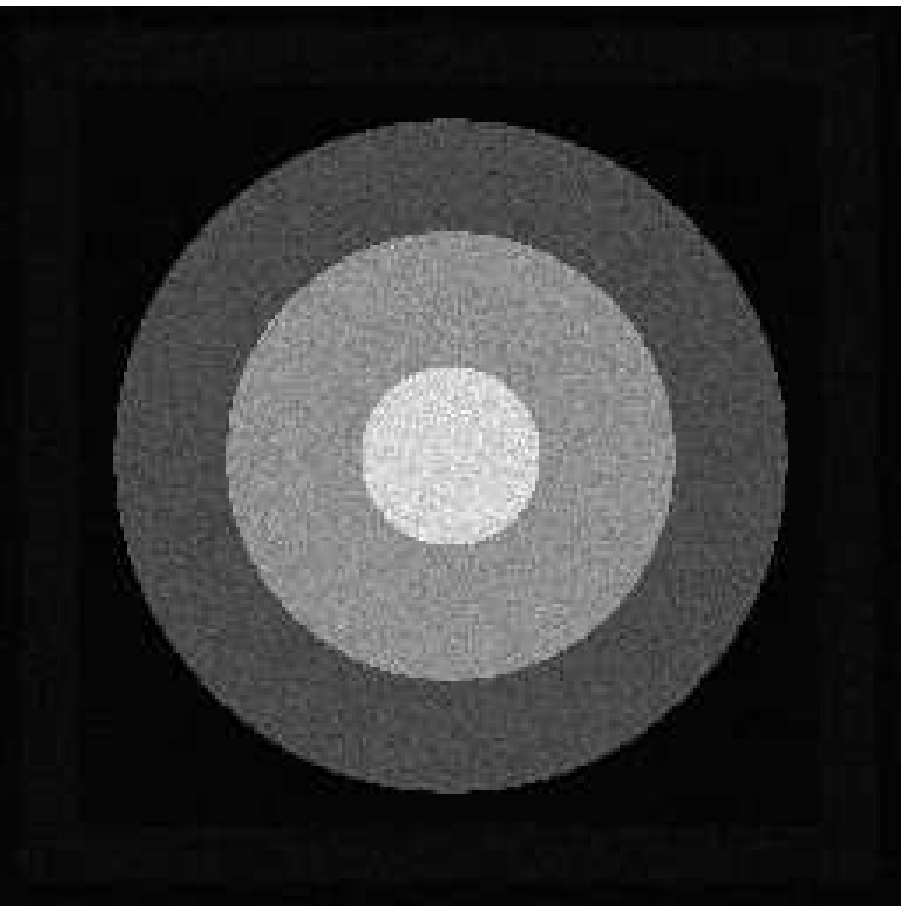
\includegraphics[width=6 cm]{img/circles_noisy}
\end{array}$
\end{center}
\caption{LCR-1: the original image and the noisy one}
\end{figure}

\begin{figure}[H]
\begin{center}$
\begin{array}{cc}

\includegraphics[width=6 cm]{img/circles_10} & 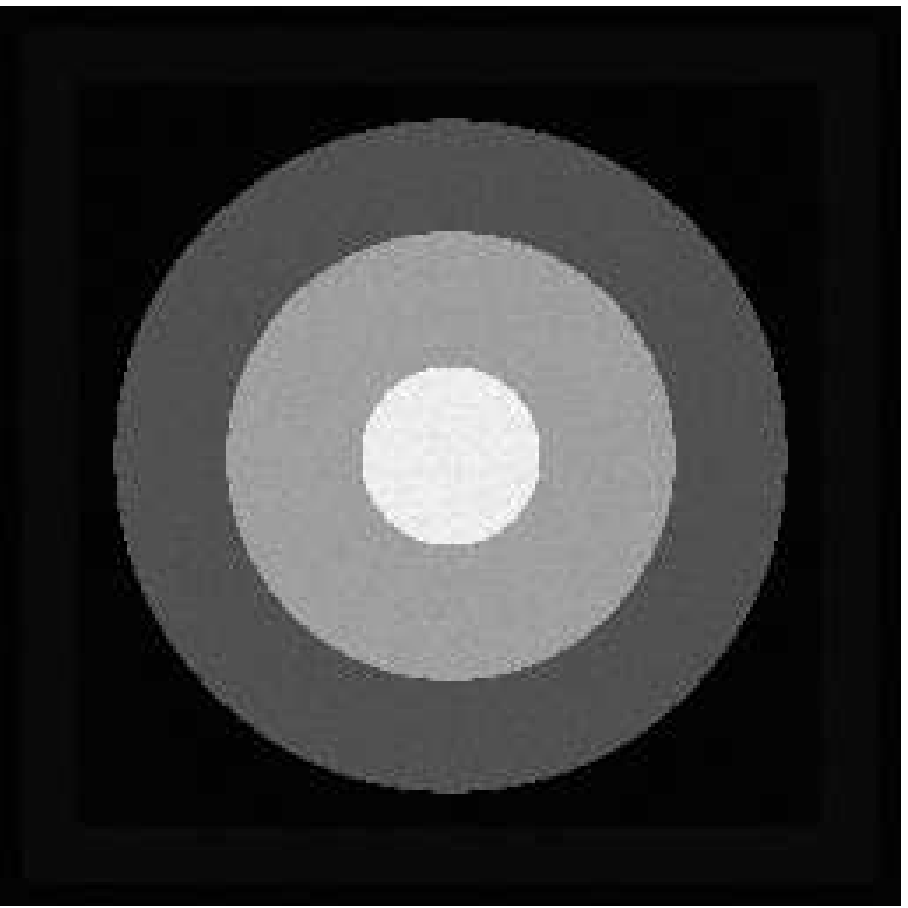
\includegraphics[width=6 cm]{img/circles_10_noisy}
\end{array}$
\end{center}
\caption{LCR-10: the original image and the noisy one}
\end{figure}

\begin{figure}[H]
\begin{center}$
\begin{array}{cc}

\includegraphics[width=6 cm]{img/circles_d5} & 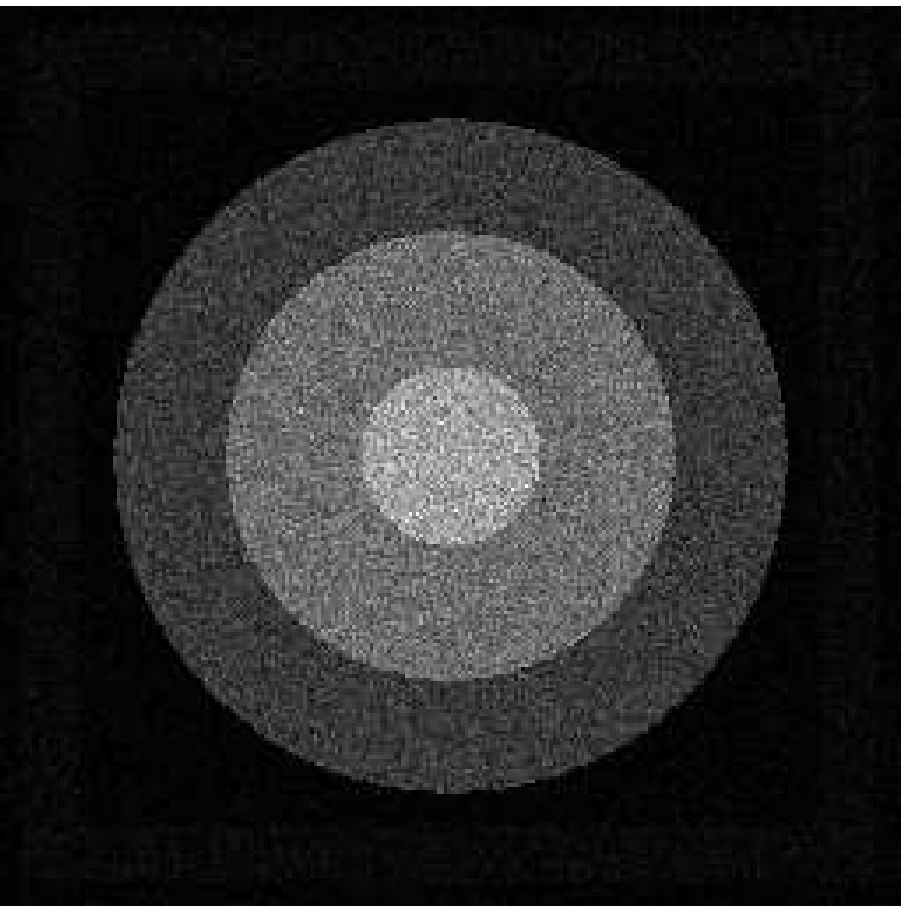
\includegraphics[width=6 cm]{img/circles_d5_noisy}
\end{array}$
\end{center}
\caption{LCR-0.2: the original image and the noisy one}
\end{figure}

\subsubsection{Airplane}
The original image is an array $256 \times 256$ depicting an aerial image of an airplane on a runway, with values in the range $[0,232]$.

\begin{figure}[H]
\begin{center}$
\begin{array}{cc}
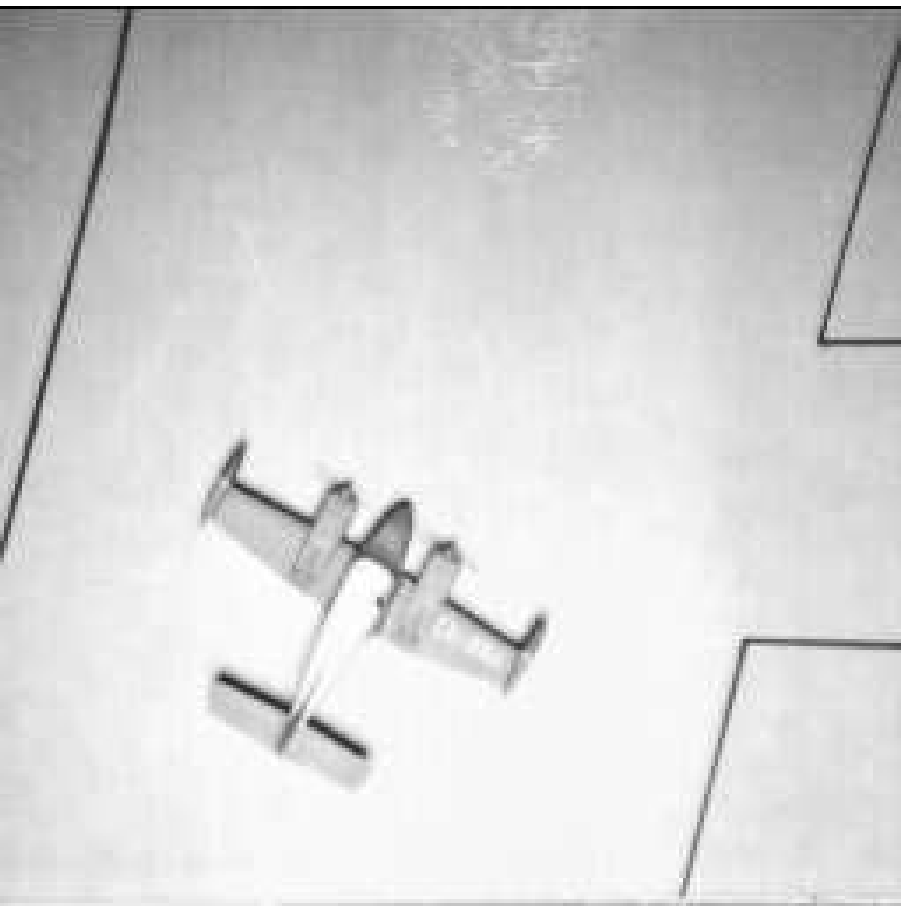
\includegraphics[width=6 cm]{img/airplane} & 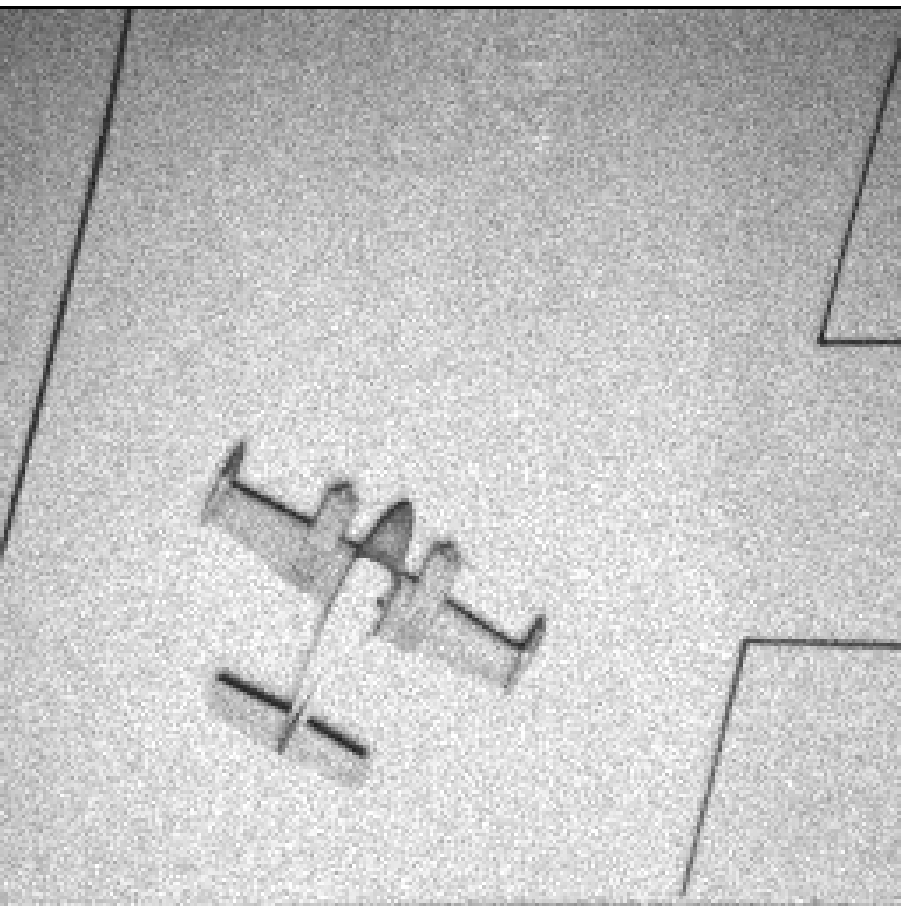
\includegraphics[width=6 cm]{img/airplane_noisy}
\end{array}$
\end{center}
\caption{Airplane: the original image and the noisy one}
\end{figure}


\subsubsection{Dental Radiography (DR)}

The original image is an array $512 \times 512$ with values in the range $[0,255]$.

\begin{figure}[H]
\begin{center}$
\begin{array}{cc}
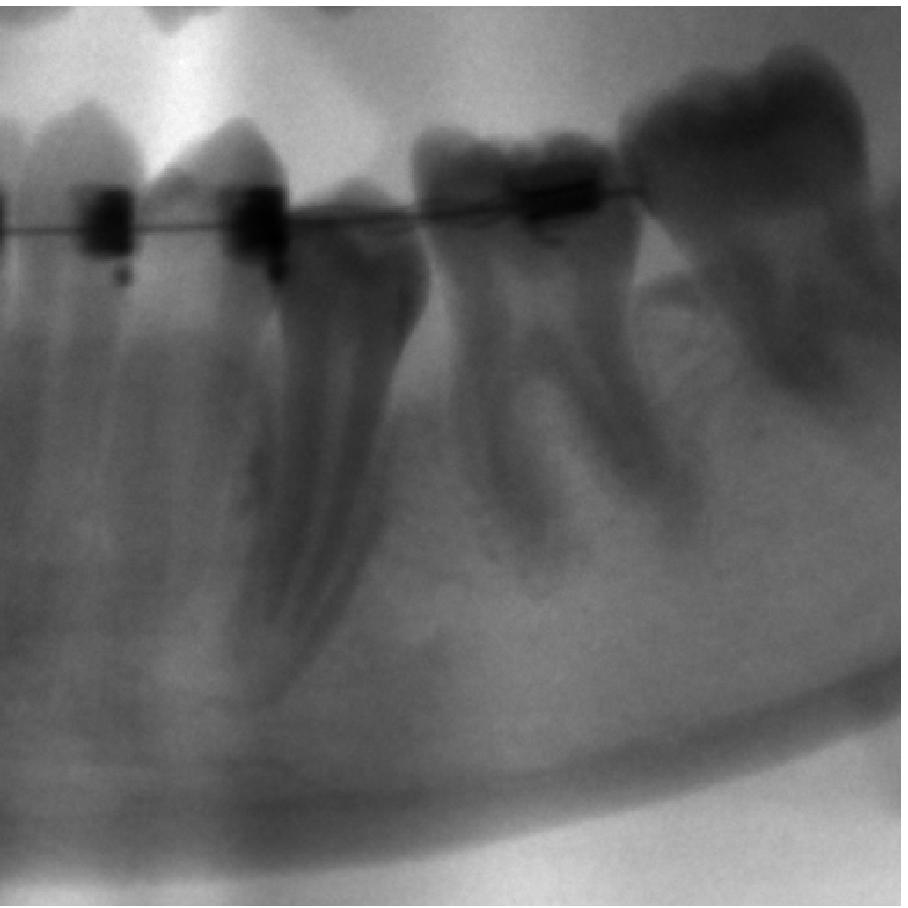
\includegraphics[width=6 cm]{img/Panoramica} & 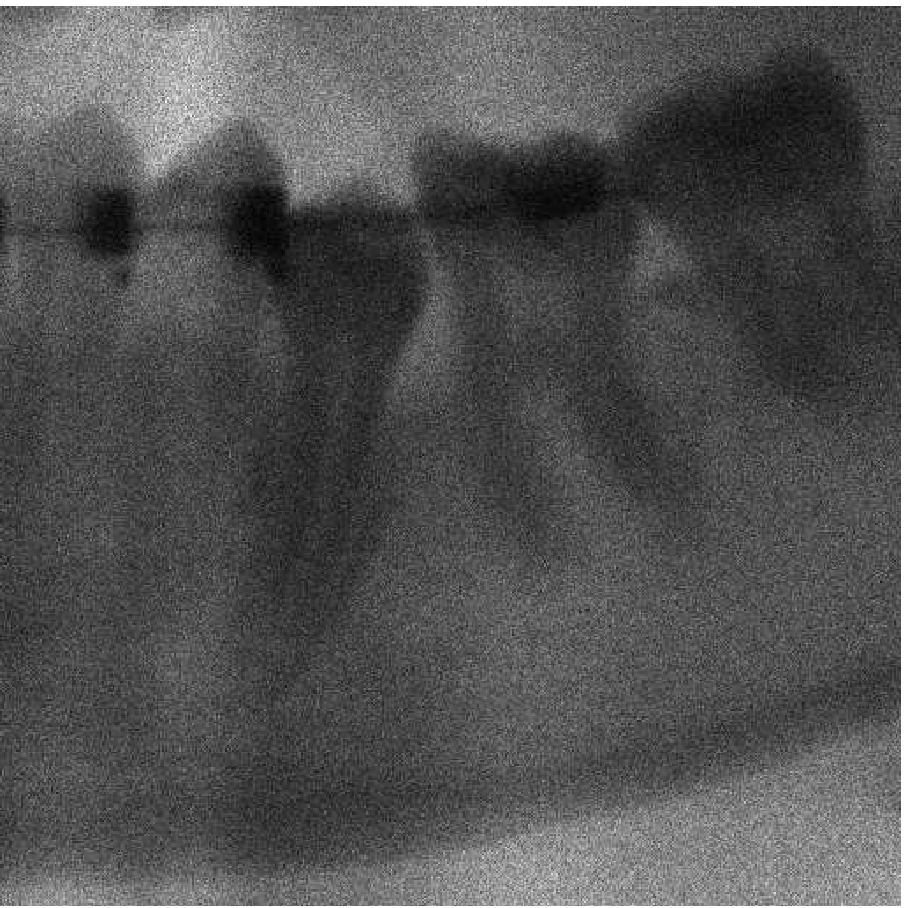
\includegraphics[width=6 cm]{img/Panoramica_noisy}
\end{array}$
\end{center}
\caption{DR: the original image and the noisy one}
\end{figure}

\subsection{Real-world problems}

As an example of problems that occurs in real world, we studied a number of images (\verb|Image11|, \verb|Image13|, \verb|Image22|, \verb|Image48|, \verb|Image49|, \verb|Image50|) from the project ``PRISMA''\footnote{See \url{http://www.unife.it/prisma}.} (optimizAtion Methods and Software for Inverse PRoblems) which represent dental radiographies affected by Poisson noise.

Every image is a ``negative'' array of $266 \times 266$ meaning that the level 4095 stands for 0 photon collected, whereas 0 stands for sensor saturation.

To obtain an image in which the gray level is linear with respect to the number of photon collected, the following transformation (with $X$ as the image array) has been used:

$$ Z = 4095 - X$$

An important difference between the simulated problems and these real ones, is that for the formers we had a noise-free image, while for the latters we do not. For this reason, a provided ``ground truth'' image has been used.

\begin{figure}[H]
\begin{center}
\includegraphics[width=6cm]{img/avg}
\end{center}
\caption{Ground truth.}
\end{figure}

\begin{figure}[H]
\begin{center}$
\begin{array}{cc}
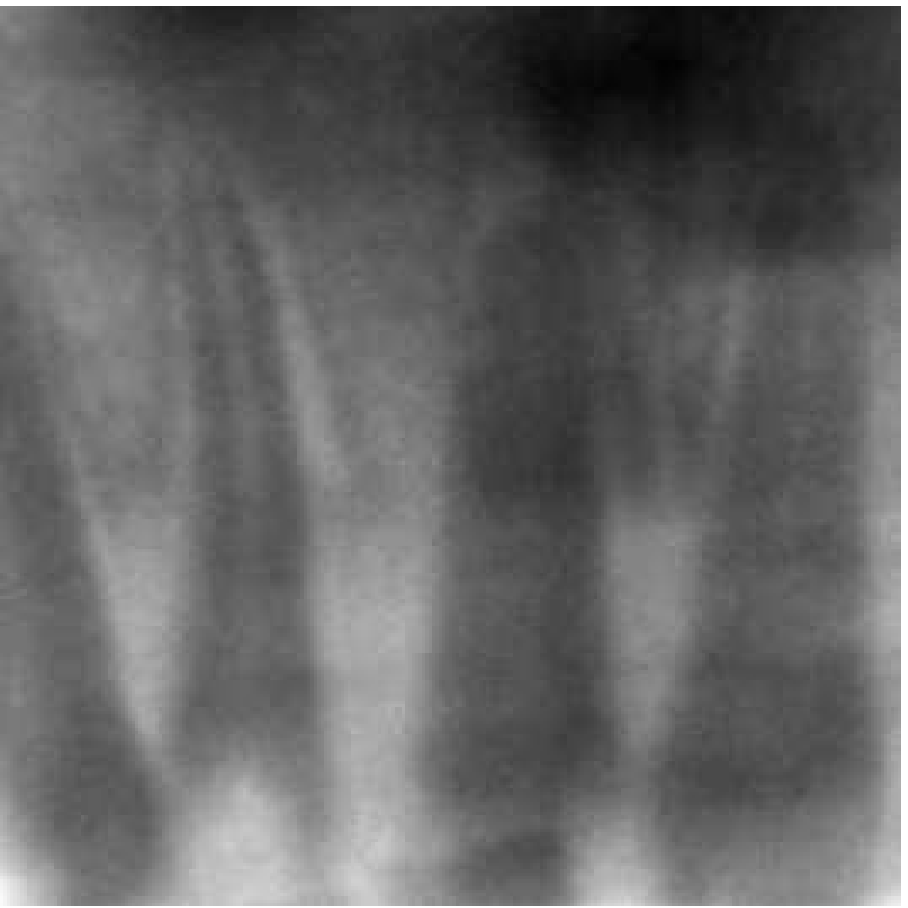
\includegraphics[width=6cm]{img/11}  & 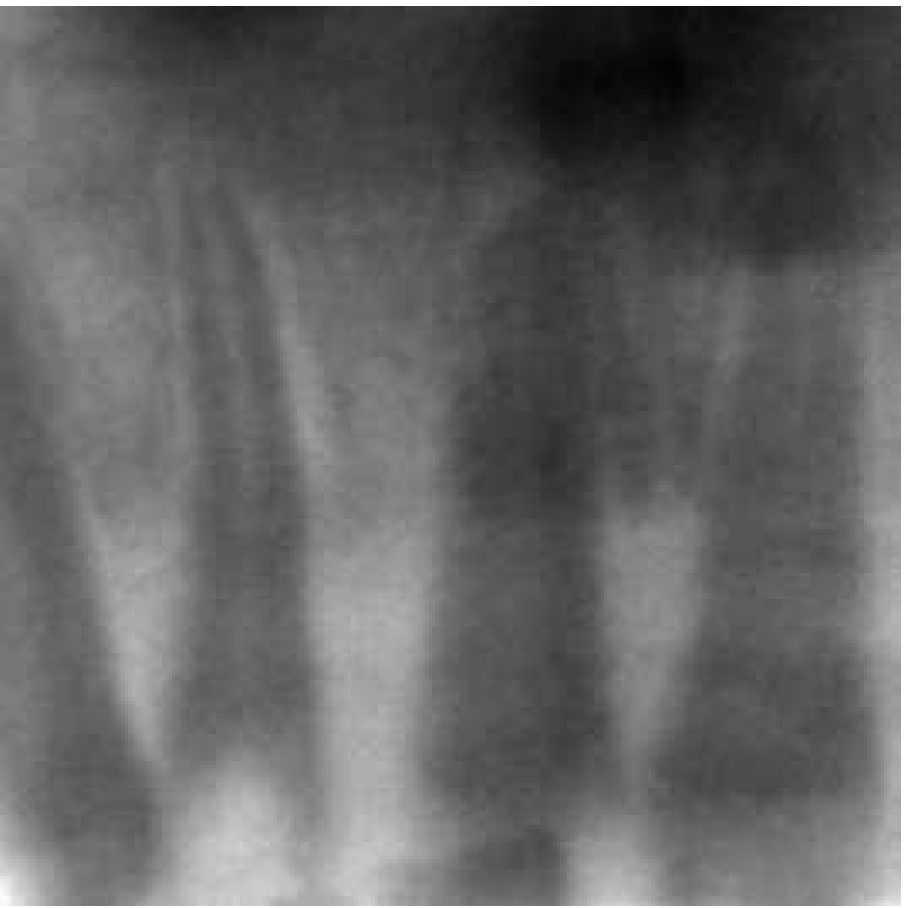
\includegraphics[width=6cm]{img/13}
\\
\mbox{Image11} & \mbox{Image 13}
\end{array}$
\end{center}
\end{figure}

\begin{figure}[H]
\begin{center}$
\begin{array}{cc}
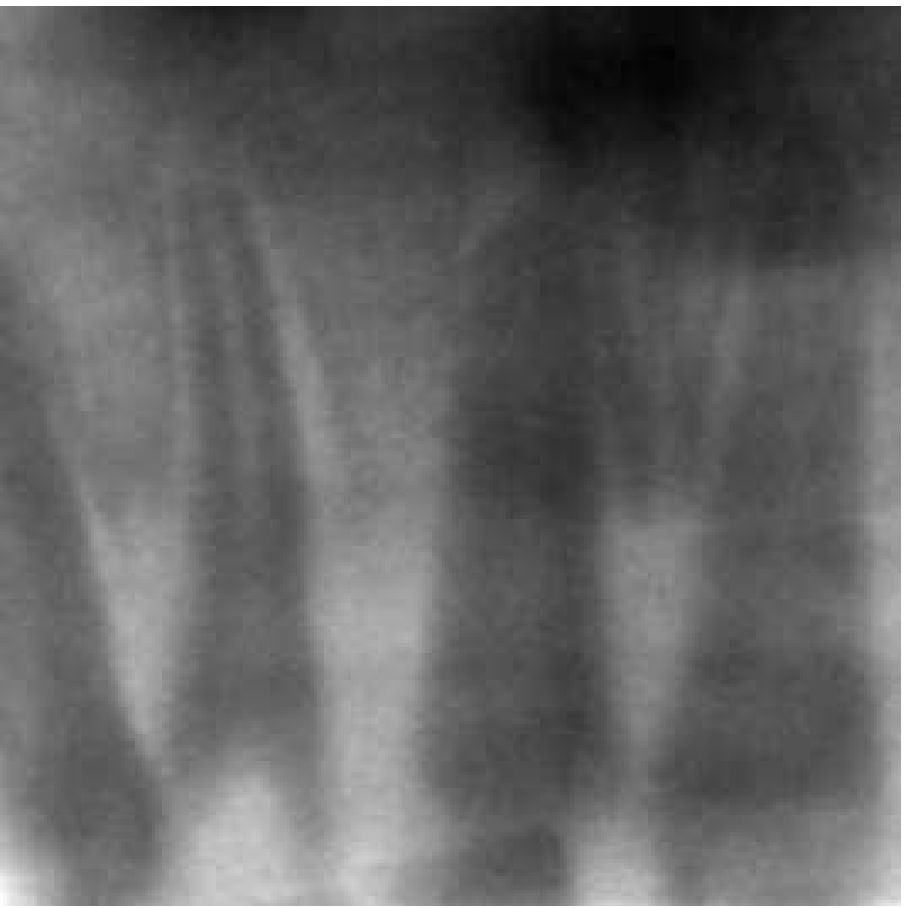
\includegraphics[width=6cm]{img/22}  & 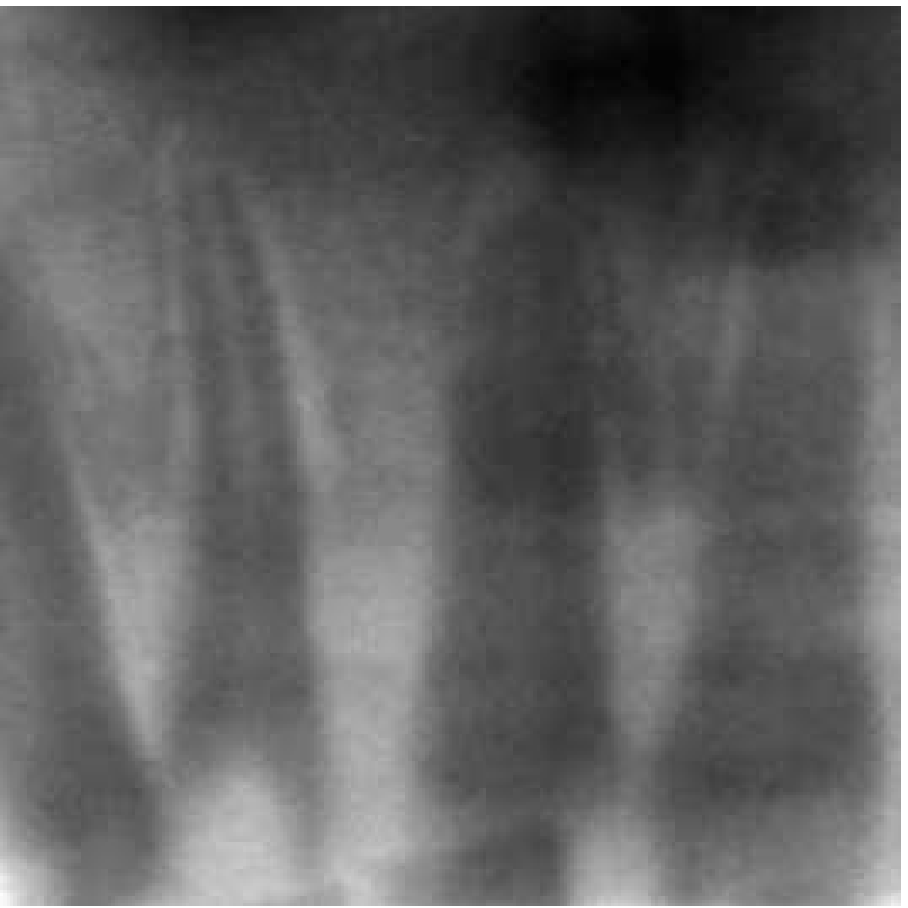
\includegraphics[width=6cm]{img/48}
\\
\mbox{Image22} & \mbox{Image 48}
\end{array}$
\end{center}
\end{figure}

\begin{figure}[H]
\begin{center}$
\begin{array}{cc}

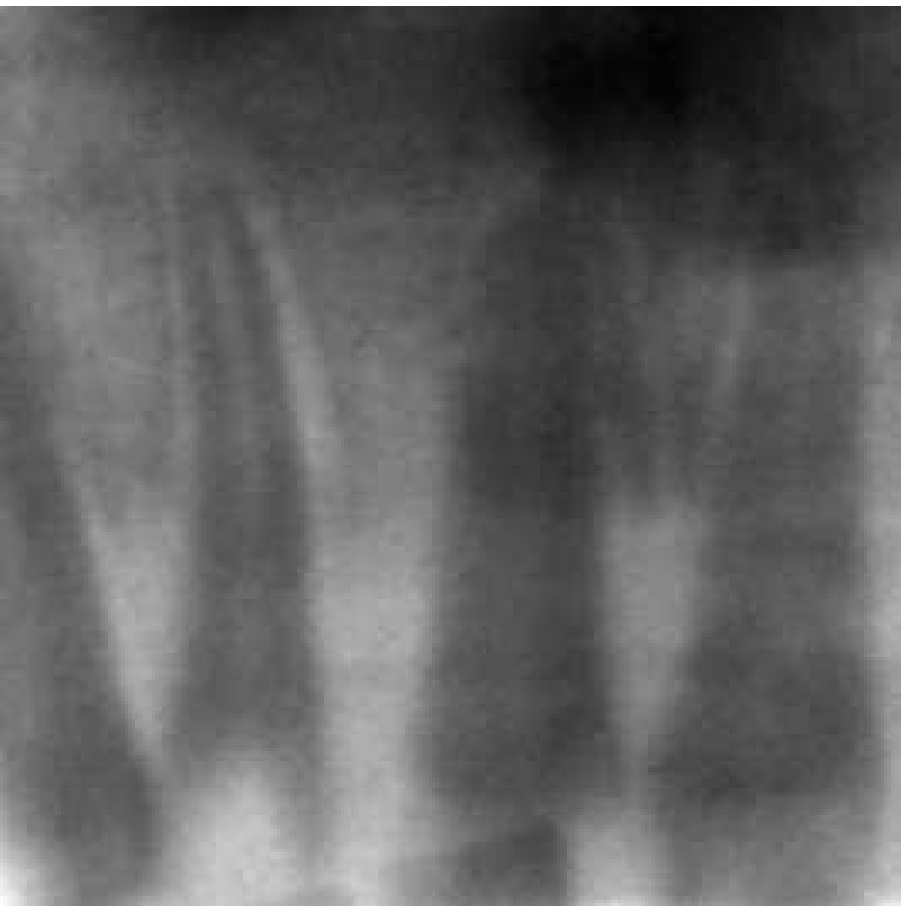
\includegraphics[width=6cm]{img/49}  & 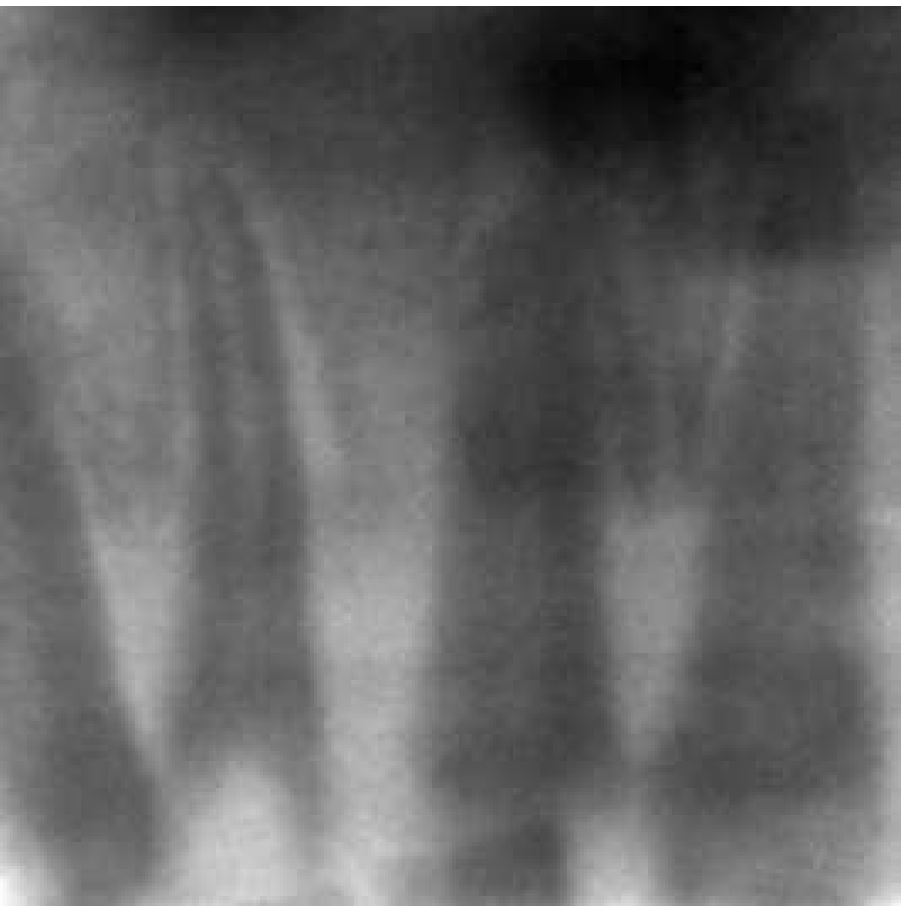
\includegraphics[width=6cm]{img/50}
\\
\mbox{Image49} & \mbox{Image 50}
\end{array}$
\end{center}
\end{figure}

\section{Numerical stability of AEM and PIDSplit+}

In the first set of experiments we compare the numerical behavior of the methods previously described, PIDSplit+ and AEM, on the five denoising problems LCR-1, LCR-10, LCR-0.2, Airplane, and DR.

To get the ideal solution $\tilde{x}$ of the minimization problem, we run AEM until 10000 iterations are reached.

Both the algorithms have been initialized with $x^{(0)} = max\{\eta,f\}$, where the maximum is meant component-wise, $\eta$ is the same as in \eqref{domain} and $f$ is the noisy image. The initial guess for the dual variable $y^{(0)}$ for AEM has been set to zero.

The values of $\beta$ used for each problem in \eqref{map}, as suggested in \citep{zanella}, are shown in the following table:

\begin{table}[H]
\begin{center}
\renewcommand*{\arraystretch}{1.4}
\begin{tabular}{m{1.8cm}|m{1cm}}
Problem & $\beta$ \\
\hline
LCR-1 & 0.25 \\
\hline
LCR-10 & 0.05 \\
\hline
LCR-0.2 & 0.575 \\
\hline
Airplane & 0.05 \\
\hline
DR & 0.27 \\
\end{tabular}
\caption{Values of $\beta$}
\end{center}
\end{table}

Since the value of $\gamma$ required by the PIDSplit+ algorithm is a user-supplied parameter which depends on the problem, we choose the values shown in the table below, along with the name used to refer to the PIDSplit+ algorithm with a particular value of $\gamma$.

\begin{table}[H]
\begin{center}
\renewcommand*{\arraystretch}{1.8}
\begin{tabular}{C{0.8cm}|C{1cm}}
$\gamma$ & Label \\
\hline
$50/\beta$ & PID50 \\
\hline
$5/\beta$ & PID5 \\
\hline
$1/\beta$ & PID1 \\
\hline
$0.5/\beta$ & PID05 \\
\end{tabular}
\caption{Values of $\gamma$ and the labels used.}
\end{center}
\end{table}

In order to evaluate the accuracy of the results and the effectiveness of the methods, in the following tables we report the iteration (\emph{iter}) and time ($t^{(iter)}$) in seconds required to reach a particular threshold of relative error, defined as

$$\epsilon^{(iter)} = \dfrac{\left|\left|x^{(iter)}-\tilde{x}\right|\right|_2}{\left|\left|\tilde{x}\right|\right|_2}$$

where $iter$ is the iteration number and $\tilde{x}$ is the approximate solution of the minimization problem, as described previously.

Furthermore, we define the relative reconstruction error:

$$e^{(iter)} = \dfrac{\left|\left|x^{(iter)}-x^*\right|\right|_2}{\left|\left|x^*\right|\right|_2}$$

where $x^*$ is the original, noise-free, image.

An empty cell in the following tables indicates that the particular error threshold $\epsilon$ has not been reached in 3000 iterations.

\begin{table}[H]
\begin{center}
\renewcommand*{\arraystretch}{1.5}
\begin{tabular}{|C{1.2cm}|C{0.9cm}|C{0.9cm}|C{1.5cm}|C{0.9cm}|C{0.9cm}|C{1.5cm}|}\hline

Method & \multicolumn{3}{c|} {$\epsilon = 10^{-2}$}  & \multicolumn{3}{c|} {$\epsilon = 10^{-4}$} \\ \cline{2-7}
     & \emph{iter} & $t^{(iter)}$ & $e^{(iter)}$ & \emph{iter} & $t^{(iter)}$  & $e^{(iter)}$  \\ \hline
AEM & 64 & 3.45 & 0.0230578 & 605 & 29.91 & 0.0249536   \\ \hline
PID50 & 65 & 3.47 & 0.0277052 & & &  \\ \hline
PID5 & 27 & 1.42 & 0.0250464 & 1023 & 57.9 & 0.0249536    \\ \hline
PID1 & 82 & 4.43 & 0.022816 & 594 & 33.43 & 0.0249649 \\ \hline
PID05 & 158 & 9.17 & 0.0226965 & 1183 & 66.91 & 0.0249641  \\ \hline
     & \multicolumn{3}{c|} {$\epsilon = 10^{-5}$}  & \multicolumn{3}{c|} {$\epsilon = 5\cdot 10^{-6}$}  \\ \cline{2-7}
     & \emph{iter} & $t^{(iter)}$  & $e^{(iter)}$ & \emph{iter} & $t^{(iter)}$  & $e^{(iter)}$ \\ \hline
AEM   & 1943 & 96.67 & 0.0249837 & & &  \\ \hline
PID50 & & & & & &  \\ \hline
PID5  & & & & & &  \\ \hline
PID1  & 1029 & 58.08 & 0.0249835 & 1478 & 83.33 & 0.0249836  \\ \hline
PID05 & 1932 & 109.24 & 0.0249832 & 2186 & 124.34 & 0.249834 \\ \hline
\end{tabular}
\caption{Results for LCR-1}
\label{tab:err2}
\end{center}
\end{table}

\begin{table}[H]
\begin{center}
\renewcommand*{\arraystretch}{1.5}
\begin{tabular}{|C{1.2cm}|C{1cm}|C{2.2cm}|C{1.5cm}|}\hline
Method & $t^{(3000)}$ & $\epsilon^{(3000)}$ & $e^{(3000)}$ \\ \hline
AEM &  149.91 & $6.3934 \cdot 10^{-6}$ & 0.0249836 \\ \hline
PID50 &  167.23 & $3.30784 \cdot 10^{-4}$ & 0.0249921 \\ \hline
PID5 &  170.81 & $1.86697 \cdot 10^{-5}$ & 0.0249839 \\ \hline
PID1 &  169.24 & $2.40734 \cdot 10^{-6}$ & 0.0249835 \\ \hline
PID05 &  169.9 & $1.0246 \cdot 10^{-6}$ & 0.0249835 \\ \hline
\end{tabular}
\caption{Results for LCR-1 after 3000 iterations.}
\end{center}
\end{table}

%% inizio lcr-10

\begin{table}[H]
\begin{center}
\renewcommand*{\arraystretch}{1.5}
\begin{tabular}{|C{1.2cm}|C{0.9cm}|C{0.9cm}|C{1.7cm}|C{0.9cm}|C{0.9cm}|C{1.7cm}|}\hline
Method & \multicolumn{3}{c|} {$\epsilon = 10^{-2}$}  & \multicolumn{3}{c|} {$\epsilon = 10^{-4}$} \\ \cline{2-7}
     & \emph{iter} & $t^{(iter)}$  & $e^{(iter)}$ & \emph{iter} & $t^{(iter)}$  & $e^{(iter)}$  \\ \hline
AEM & 92 & 4.65 & 0.0118767 & 816 & 40.9 & 0.00835666   \\ \hline
PID50 & 5 & 0.22 & 0.0110561 & 540 &  30.13 & 0.00838595  \\ \hline
PID5 & 24 & 1.24 & 0.00119889 & 320 & 17.94 & 0.00833781    \\ \hline
PID1 & 116 & 6.39 & 0.0119236 & 1592 & 96.69 & 0.00833768 \\\hline
     & \multicolumn{3}{c|} {$\epsilon = 10^{-5}$}  & \multicolumn{3}{c|} {$\epsilon = 5\cdot 10^{-6}$}  \\ \cline{2-7}
     & \emph{iter} & $t^{(iter)}$  & $e^{(iter)}$ & \emph{iter} & $t^{(iter)}$  & $e^{(iter)}$ \\ \hline
AEM   & 1360 & 66.87 & 0.00838057 & 1531 & 74.92 & 0.00838169  \\ \hline
PID50 & 2622 & 146.63 & 0.00838286 & & &  \\ \hline
PID5  &  558 & 31.19 & 0.00837926 &  654 &  36.6 & 0.00838144  \\ \hline
PID1  & 2731 & 153.58 & 0.00837883 & & &  \\ \hline
\end{tabular}
\caption{Results for LCR-10}
\end{center}
\end{table}

\begin{table}[H]
\begin{center}
\renewcommand*{\arraystretch}{1.5}
\begin{tabular}{|C{1.2cm}|C{1cm}|C{2.2cm}|C{1.7cm}|}\hline
Method & $t^{(3000)}$ & $\epsilon^{(3000)}$ & $e^{(3000)}$ \\ \hline
AEM &  143.01 & $2.23187 \cdot 10^{-7}$ & 0.00838268 \\ \hline
PID50 &  167.66 & $8.25419 \cdot 10^{-6}$ & 0.00838283 \\ \hline
PID5 &  169.4 & $7.34523 \cdot 10^{-7}$ & 0.00838268 \\ \hline
PID1 &  169.15 & $5.8626 \cdot 10^{-6}$ & 0.00832767 \\ \hline
\end{tabular}
\caption{Results for LCR-10 after 3000 iterations.}
\end{center}
\end{table}

%% inizio lcr-0.2

\begin{table}[H]
\begin{center}
\renewcommand*{\arraystretch}{1.5}
\begin{tabular}{|C{1.2cm}|C{0.9cm}|C{0.9cm}|C{1.7cm}|C{0.9cm}|C{0.9cm}|C{1.7cm}|}\hline


Method & \multicolumn{3}{c|} {$\epsilon = 10^{-2}$}  & \multicolumn{3}{c|} {$\epsilon = 10^{-4}$} \\ \cline{2-7}
     & \emph{iter} & $t^{(iter)}$  & $e^{(iter)}$ & \emph{iter} & $t^{(iter)}$  & $e^{(iter)}$  \\ \hline
AEM & 102 & 5.97 & 0.0441267 & 2104 & 113.06 & 0.0447745   \\ \hline
PID50 & 478 & 25.79 & 0.0465756 &  &  &  \\ \hline
PID5 & 60 & 3.04 & 0.0466034 & & &    \\ \hline
PID1 & 68 & 3.76 & 0.0438891 & 696 & 37.92 & 0.0447745 \\\hline
PID05 & 119 & 6.50 & 0.0432181 & 606 & 33.01 & 0.0447726 \\\hline
     & \multicolumn{3}{c|} {$\epsilon = 10^{-5}$}  & \multicolumn{3}{c|} {$\epsilon = 5\cdot 10^{-6}$}  \\ \cline{2-7}
     & \emph{iter} & $t^{(iter)}$  & $e^{(iter)}$ & \emph{iter} & $t^{(iter)}$  & $e^{(iter)}$ \\ \hline
AEM   & & & & & &  \\ \hline
PID50 & & & & & &  \\ \hline
PID5  & & & & & & \\ \hline
PID1  & 1418 & 77.80 & 0.044773 & 1591 & 87.5 & 0.047729 \\ \hline
PID05  & & & & & & \\ \hline
\end{tabular}
\caption{Results for LCR-0.2}
\end{center}
\end{table}

\begin{table}[H]
\begin{center}
\renewcommand*{\arraystretch}{1.5}
\begin{tabular}{|C{1.2cm}|C{1cm}|C{2.2cm}|C{1.7cm}|}\hline
Method & $t^{(3000)}$ & $\epsilon^{(3000)}$ & $e^{(3000)}$ \\ \hline
AEM &  160.72 & $4.42311 \cdot 10^{-5}$ & 0.0447735 \\ \hline
PID50 &  164.51 & $1.00901 \cdot 10^{-3}$ & 0.0448293 \\ \hline
PID5 &  165.22 & $1.34896 \cdot 10^{-4}$ & 0.0447752 \\ \hline
PID1 &  164.91 & $1.80577 \cdot 10^{-5}$ & 0.0447724 \\ \hline
PID05 &  164.95 & $2.79695 \cdot 10^{-5}$ & 0.0447722 \\ \hline
\end{tabular}
\caption{Results for LCR-0.2 after 3000 iterations.}
\end{center}
\end{table}

%% inizio airplane

\begin{table}[H]
\begin{center}
\renewcommand*{\arraystretch}{1.5}
\begin{tabular}{|C{1.2cm}|C{0.9cm}|C{0.9cm}|C{1.7cm}|C{0.9cm}|C{0.9cm}|C{1.7cm}|}\hline


Method & \multicolumn{3}{c|} {$\epsilon = 10^{-2}$}  & \multicolumn{3}{c|} {$\epsilon = 10^{-4}$} \\ \cline{2-7}
     & \emph{iter} & $t^{(iter)}$  & $e^{(iter)}$ & \emph{iter} & $t^{(iter)}$  & $e^{(iter)}$  \\ \hline
AEM & 68 & 3.32 & 0.0258942 & 192 & 9.02 & 0.0214011   \\ \hline
PID50 & 7 & 0.33 & 0.0227146 & 451 & 25.82  & 0.0213743 \\ \hline
PID5 & 18 & 0.96 & 0.0252871 & 75 & 4.23 & 0.0213782   \\ \hline
PID1 & 82 & 4.53 & 0.0258994 & 324 & 17.98 & 0.0213914 \\ \hline
PID05 & 163 & 9.06 & 0.0258684 & 646 & 36.93 & 0.0213913 \\ \hline
     & \multicolumn{3}{c|} {$\epsilon = 10^{-5}$}  & \multicolumn{3}{c|} {$\epsilon = 5\cdot 10^{-6}$}  \\ \cline{2-7}
     & \emph{iter} & $t^{(iter)}$  & $e^{(iter)}$ & \emph{iter} & $t^{(iter)}$  & $e^{(iter)}$ \\ \hline
AEM   & 266 & 12.86 & 0.0213756 & 350 & 17.03 & 0.0213742  \\ \hline
PID50 & & & & & &  \\ \hline
PID5  & 362 & 20.63 & 0.0213741 & 679 & 38.41 & 0.0213742 \\ \hline
PID1  & 481 & 26.78 & 0.0213754 & 534 & 30.02 & 0.0213748 \\ \hline
PID05 & 956 & 54.98 & 0.0213754 & 1056 & 60.53 & 0.0213748 \\ \hline
\end{tabular}
\caption{Results for Airplane}
\end{center}
\end{table}

\begin{table}[H]
\begin{center}
\renewcommand*{\arraystretch}{1.5}
\begin{tabular}{|C{1.2cm}|C{1cm}|C{2.2cm}|C{1.7cm}|}\hline
Method & $t^{(3000)}$ & $\epsilon^{(3000)}$ & $e^{(3000)}$ \\ \hline
AEM &  148.21 & $4.66582 \cdot 10^{-7}$ & 0.0213742 \\ \hline
PID50 &  172.8 & $1.07853 \cdot 10^{-5}$ & 0.0213741 \\ \hline
PID5 &  169.26 & $1.01562 \cdot 10^{-6}$ & 0.0213742 \\ \hline
PID1 &  169.1 & $1.97154 \cdot 10^{-7}$ & 0.0213742 \\ \hline
PID05 &  171.54 & $9.10447 \cdot 10^{-8}$ & 0.0213742 \\ \hline
\end{tabular}
\caption{Results for Airplane after 3000 iterations.}
\end{center}
\end{table}

%% inizio DR

\begin{table}[H]
\begin{center}
\renewcommand*{\arraystretch}{1.5}
\begin{tabular}{|C{1.2cm}|C{0.9cm}|C{0.9cm}|C{1.7cm}|C{0.9cm}|C{0.9cm}|C{1.7cm}|}\hline


Method & \multicolumn{3}{c|} {$\epsilon = 10^{-2}$}  & \multicolumn{3}{c|} {$\epsilon = 10^{-4}$} \\ \cline{2-7}
     & \emph{iter} & $t^{(iter)}$  & $e^{(iter)}$ & \emph{iter} & $t^{(iter)}$  & $e^{(iter)}$  \\ \hline
AEM & 43 & 8.24 & 0.0275251 & 481 & 93.32 & 0.0296553   \\ \hline
PID50 & 91 & 17.86 & 0.0277751 &  &  &  \\ \hline
PID5 & 19 & 3.53 & 0.0281259 & 921 & 195.09 & 0.0296544    \\ \hline
PID1 & 47 & 9.91 & 0.0288035 & 234 & 49.92 & 0.0296558 \\\hline
PID05 & 90 & 19.26 & 0.0291545 & 378 & 80.88 & 0.0296571 \\\hline
     & \multicolumn{3}{c|} {$\epsilon = 10^{-5}$}  & \multicolumn{3}{c|} {$\epsilon = 5\cdot 10^{-6}$}  \\ \cline{2-7}
     & \emph{iter} & $t^{(iter)}$  & $e^{(iter)}$ & \emph{iter} & $t^{(iter)}$  & $e^{(iter)}$ \\ \hline
AEM   & & & & & &  \\ \hline
PID50 & & & & & &  \\ \hline
PID5  & & & & & & \\ \hline
PID1  & 1361 & 291.52 & 0.0296611 & 2567 & 549.45 & 0.0296614 \\ \hline
PID05 & 726 & 154.72 & 0.0296613 & 1131 & 240.76 & 0.0296614  \\ \hline
\end{tabular}
\caption{Results for DR}
\end{center}
\end{table}

\begin{table}[H]
\begin{center}
\renewcommand*{\arraystretch}{1.5}
\begin{tabular}{|C{1.2cm}|C{1cm}|C{2.2cm}|C{1.7cm}|}\hline
Method & $t^{(3000)}$ & $\epsilon^{(3000)}$ & $e^{(3000)}$ \\ \hline
AEM &  592.32 & $1.11678 \cdot 10^{-5}$ & 0.029661 \\ \hline
PID50 &  632.11 & $3.33547 \cdot 10^{-4}$ & 0.0296372 \\ \hline
PID5 &  637.26 & $2.34327 \cdot 10^{-5}$ & 0.02966 \\ \hline
PID1 &  642.70 & $4.20732 \cdot 10^{-6}$ & 0.0296615 \\ \hline
PID05 &  638.78 & $1.58306 \cdot 10^{-6}$ & 0.0296616 \\ \hline
\end{tabular}
\caption{Results for DR after 3000 iterations.}
\end{center}
\end{table}

%% inizio err2

In the following figures, we show the speed of convergence of every method in 3000 iterations, showing the relation between $\epsilon$ and the time elapsed in seconds.

\begin{figure}[H]
\begin{center}$
\begin{array}{c}
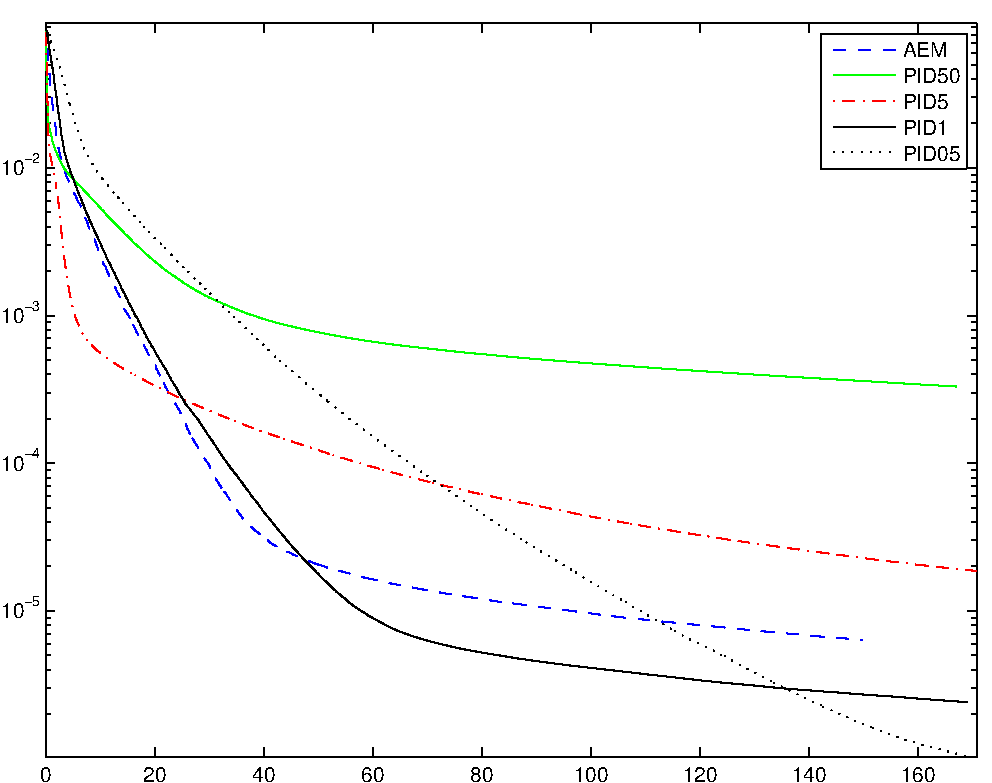
\includegraphics[width=10cm]{img/circles_err2}  \\
\mbox{LCR-1} \\
\\
\\
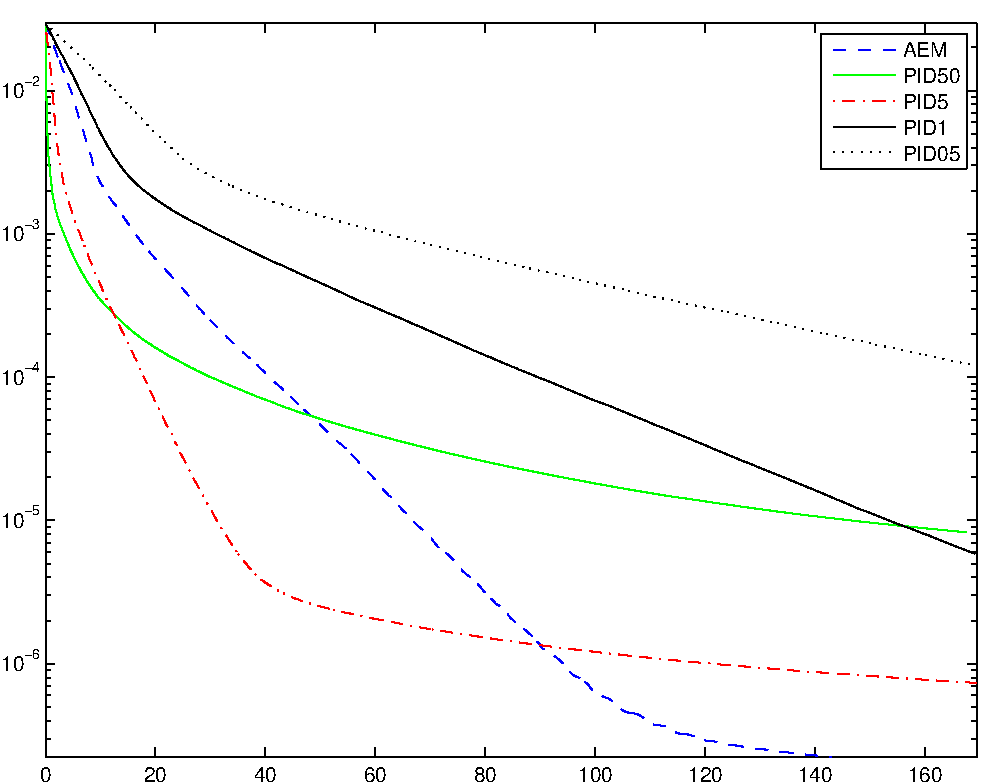
\includegraphics[width=10cm]{img/circles_10_err2} \\
\mbox{LCR-10} \\
\end{array}$
\end{center}
\end{figure}

\begin{figure}[H]
\begin{center}$
\begin{array}{cc}
\\
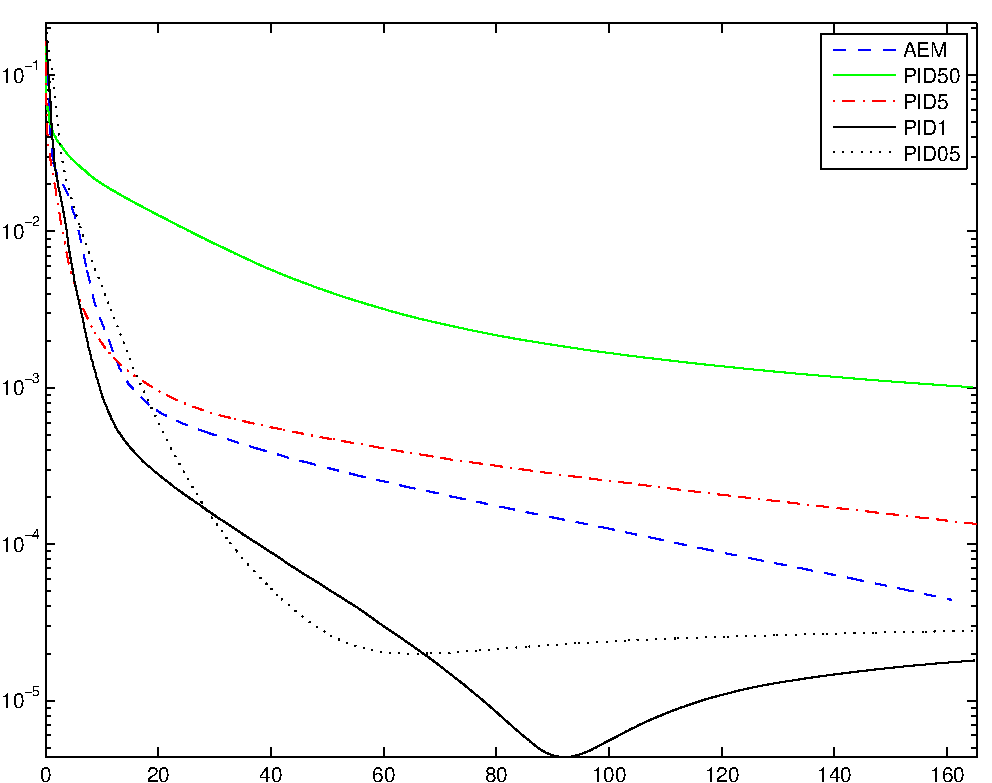
\includegraphics[width=10cm]{img/circles_d5_err2} \\
\mbox{LCR-0.2} \\
\\
\\
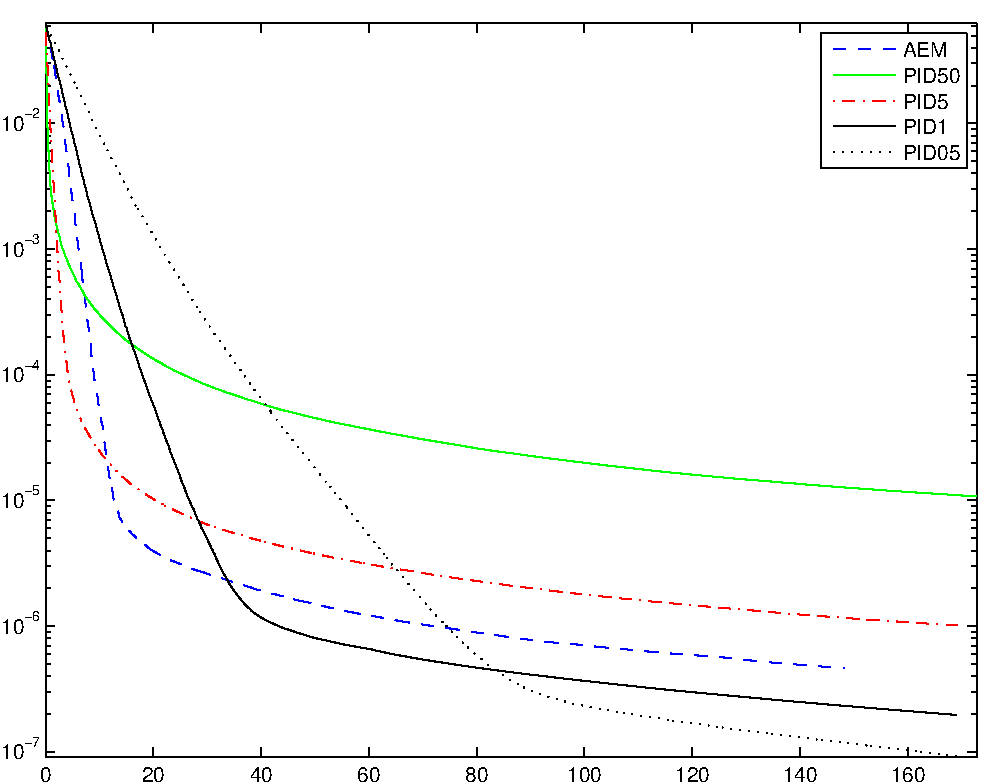
\includegraphics[width=10cm]{img/airplane_err2} \\
\mbox{Airplane} \\
\end{array}$
\end{center}
\end{figure}

\begin{figure}[H]
\begin{center}$
\begin{array}{c}
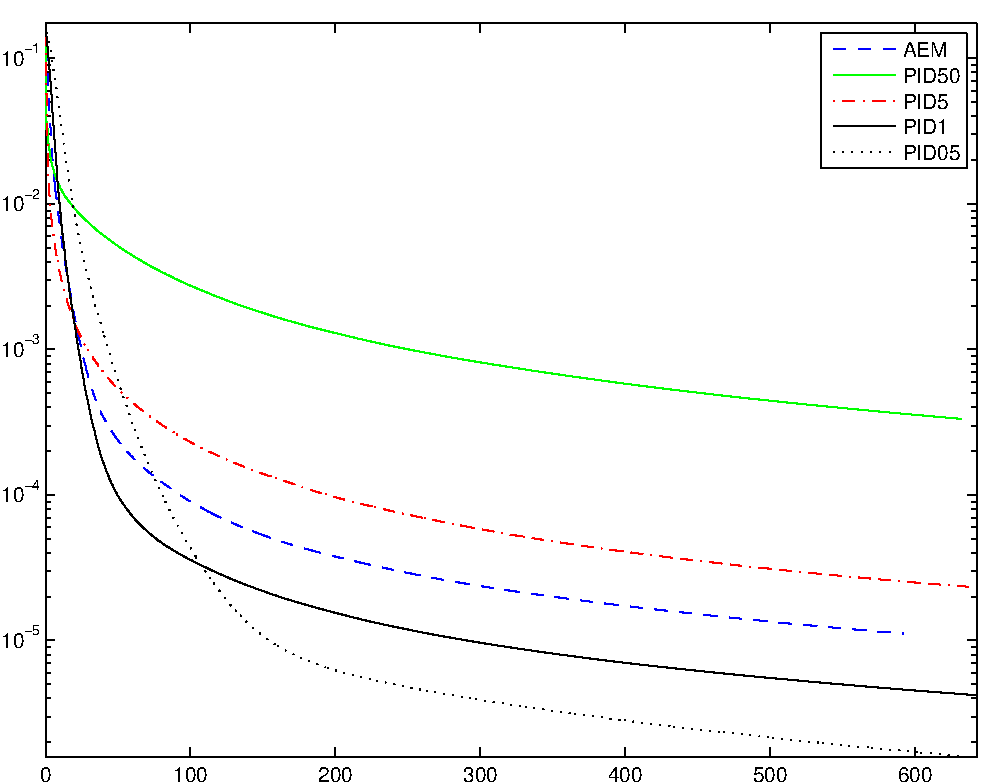
\includegraphics[width=10cm]{img/Panoramica_err2} \\
\mbox{DR} \\
\end{array}$
\end{center}
\end{figure}

%% inizio 5 sec

In order to evaluate the initial rate of convergence of the methods, we stopped both the algorithms after 5 seconds. In Table \ref{tab:5sec} we report the number of iterations performed and the corresponding reconstruction error $e$.


\begin{table}[H]
\begin{center}
\renewcommand*{\arraystretch}{1.5}
\begin{tabular}{|C{1.2cm}|C{0.9cm}|C{1.7cm}|C{0.9cm}|C{1.7cm}|C{0.9cm}|C{1.7cm}|}\hline
Method & \multicolumn{2}{c|} {LCR-1}  & \multicolumn{2}{c|} {LCR-10} & \multicolumn{2}{c|} {LCR-0.2} \\ \hline
     & \emph{iter} & $e^{(iter)}$ & \emph{iter}  & $e^{(iter)}$ & \emph{iter}  & $e^{(iter)}$ \\ \hline
AEM & 95 & 0.0236706 & 99 & 0.01113338 & 86 & 0.0444788 \\ \hline
PID50 & 90 & 0.0270578 & 91 & 0.00845165 & 98 & 0.0542035 \\ \hline
PID5 & 93 & 0.0250121 & 92 & 0.0078265 & 97 & 0.0453821 \\ \hline
PID1 & 92 & 0.0227458 & 92 & 0.0140898 & 91 & 0.0439414 \\ \hline
PID05 & 88 & 0.028708 & 93 & 0.020299 & 93 & 0.043499 \\ \hline
 & \multicolumn{2}{c|} {Airplane}  & \multicolumn{2}{c|}{DR} & \multicolumn{2}{c}{} \\ \cline{1-5}
     & \emph{iter} & $e^{(iter)}$ & \emph{iter}  & $e^{(iter)}$ & \multicolumn{2}{c}{} \\ \cline{1-5}
AEM & 109 &  0.0221838 & 27 & 0.0293069  & \multicolumn{2}{c}{} \\      \cline{1-5}
PID50 & 91 & 0.021386 & 27 & 0.0284085  & \multicolumn{2}{c}{} \\      \cline{1-5}
PID5 & 88 & 0.0213743 & 27 & 0.0286992  & \multicolumn{2}{c}{} \\      \cline{1-5}
PID1 & 91 & 0.024726 & 24 & 0.0472261  & \multicolumn{2}{c}{} \\      \cline{1-5}
PID05 & 91 & 0.0347613 & 24 & 0.0932484  & \multicolumn{2}{c}{} \\      \cline{1-5}
\end{tabular}
\caption{Number of iterations performed and reconstruction errors after 5 seconds.}
\label{tab:5sec}
\end{center}
\end{table}

In the following figures, we report the initial rate of convergence for both the algorithms, showing the relation between time and $e$ in the first 5 seconds.

\begin{figure}[H]
\begin{center}$
\begin{array}{c}
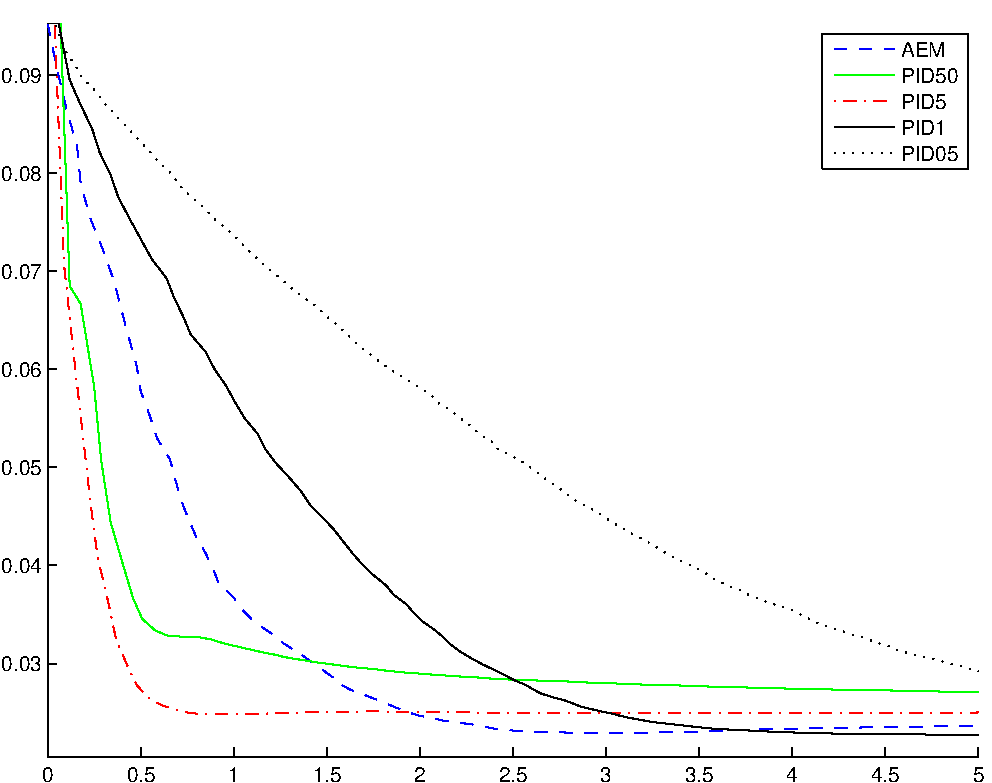
\includegraphics[width=10cm]{img/circles_err_5_sec}  \\
\mbox{LCR-1} \\
\\
\\
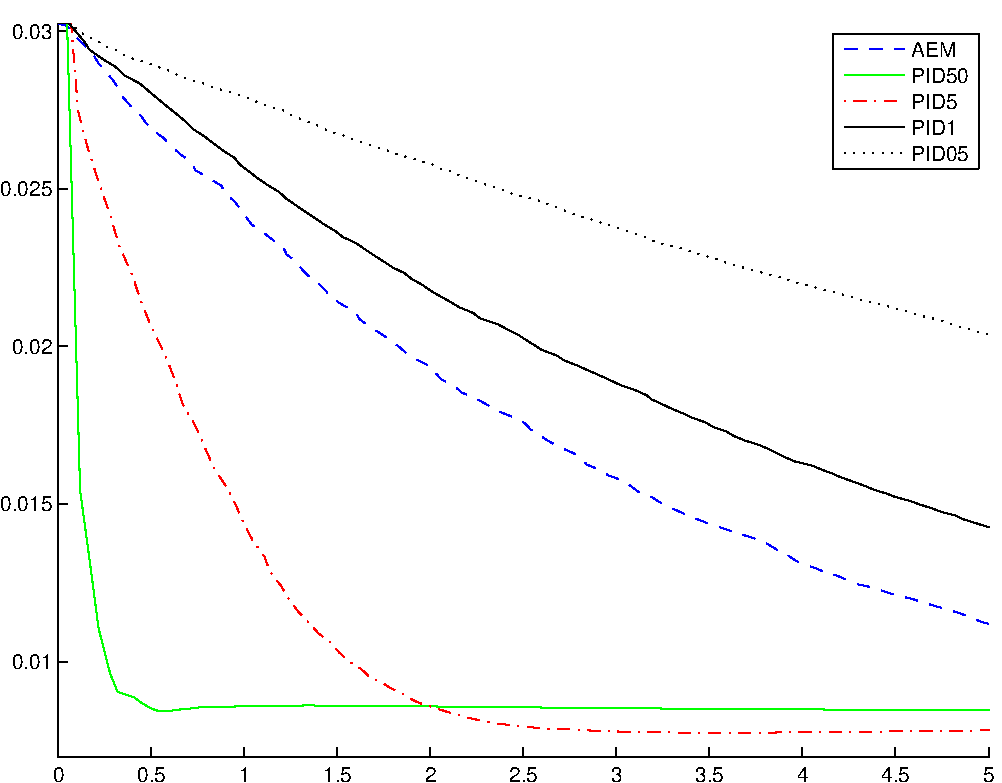
\includegraphics[width=10cm]{img/circles_10_err_5_sec} \\
\mbox{LCR-10} \\
\end{array}$
\end{center}
\caption{Behavior of relative reconstruction error in the first 5 seconds of the different methods for LCR-1 and LCR-10.}
\end{figure}

\begin{figure}[H]
\begin{center}$
\begin{array}{cc}
\\
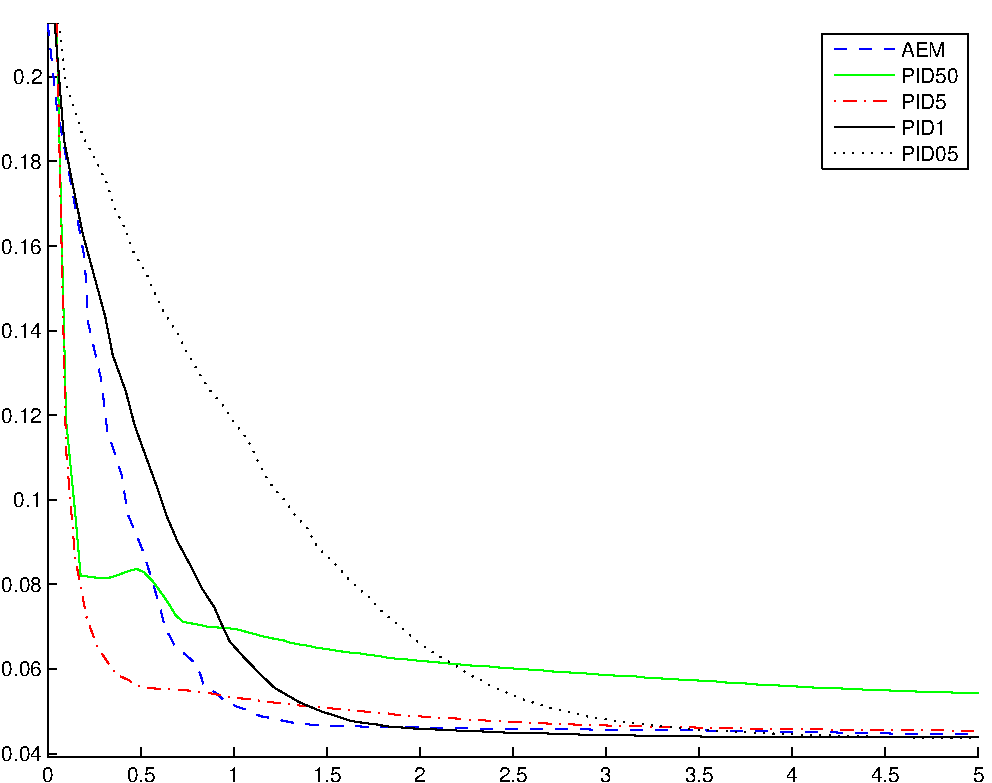
\includegraphics[width=10cm]{img/circles_d5_err_5_sec} \\
\mbox{LCR-0.2} \\
\\
\\
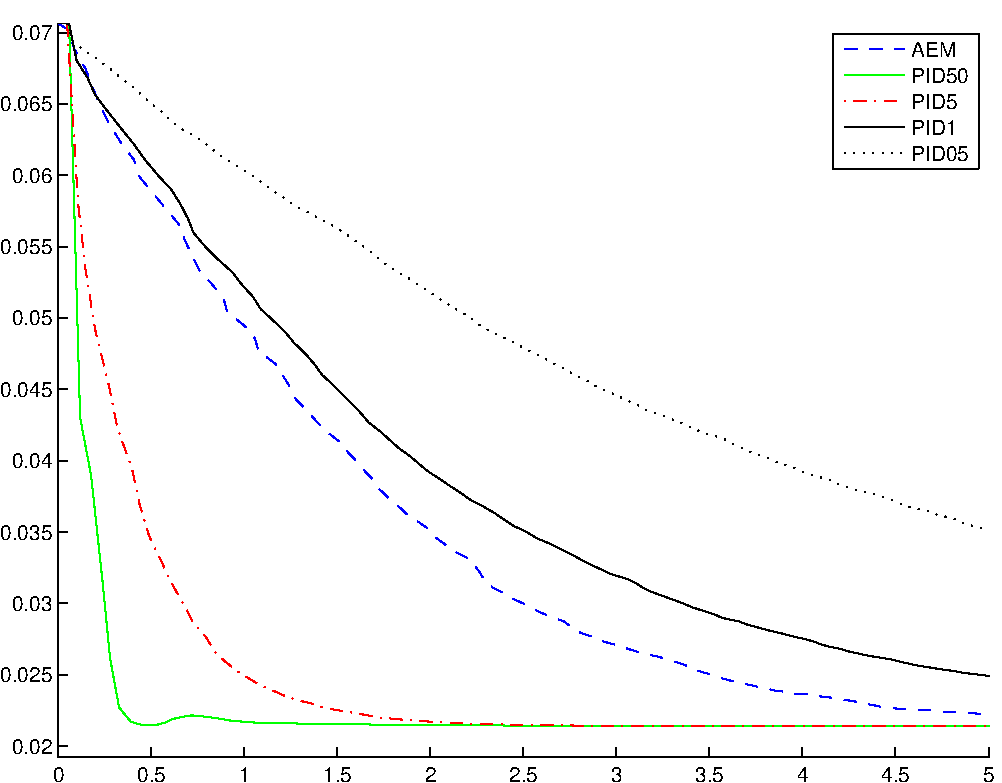
\includegraphics[width=10cm]{img/airplane_err_5_sec} \\
\mbox{Airplane} \\
\end{array}$
\end{center}
\caption{Behavior of relative reconstruction error in the first 5 seconds of the different methods for LCR-0.2 and Airplane.}
\end{figure}

\begin{figure}[H]
\begin{center}$
\begin{array}{c}
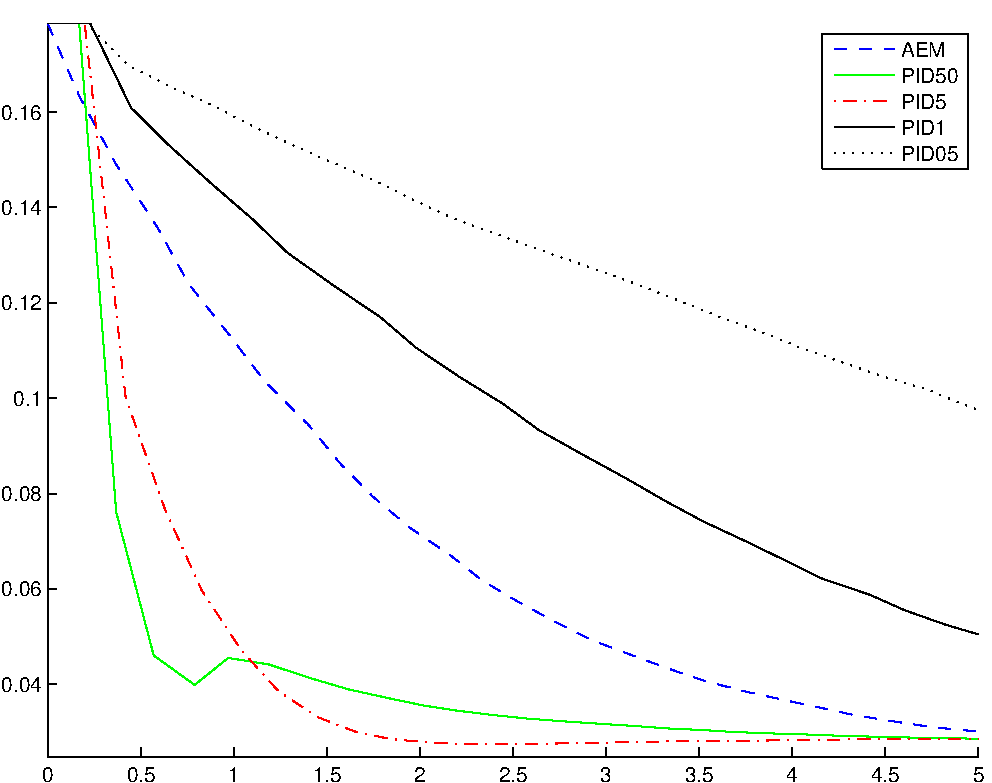
\includegraphics[width=10cm]{img/Panoramica_err_5_sec} \\
\mbox{DR} \\
\end{array}$
\end{center}
\caption{Behavior of relative reconstruction error in the first 5 seconds of the different methods for DR.}
\end{figure}

In order to evaluate if 5 seconds are enough to determine a good reconstruction of the image, we report the results after 5 seconds. For LCR-1, LCR-10, LCR-0.2, instead of the resulting image, we show the relation between the number of the column and the intensity, for the line 128.

\begin{figure}[H]
\begin{center}$
\begin{array}{cc}
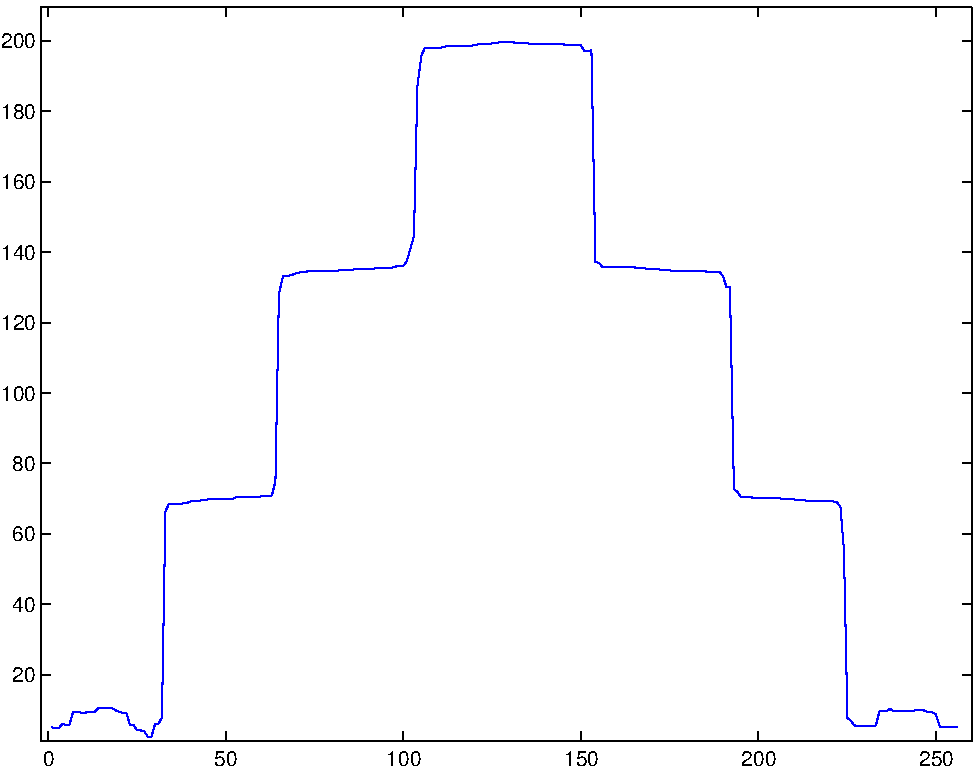
\includegraphics[width=6cm]{img/circles_it_95} & 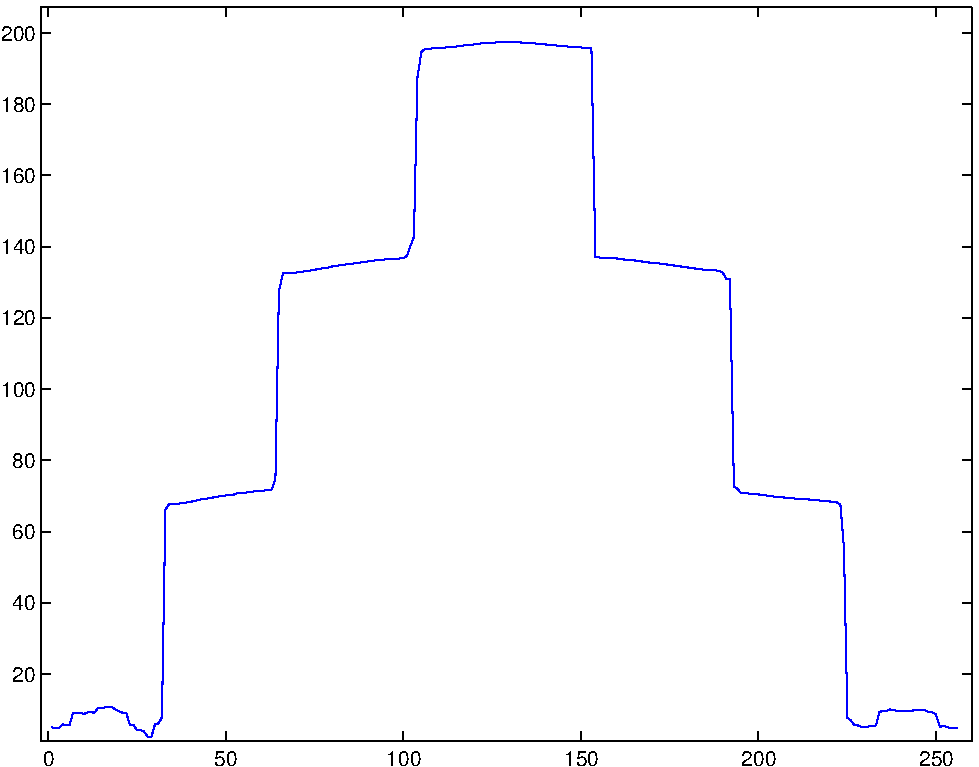
\includegraphics[width=6cm]{img/circles_PID_50_it_90} \\
\\
\mbox{AEM: 95 iterations} & \mbox{PID50: 90 iterations} \\
\\
\\
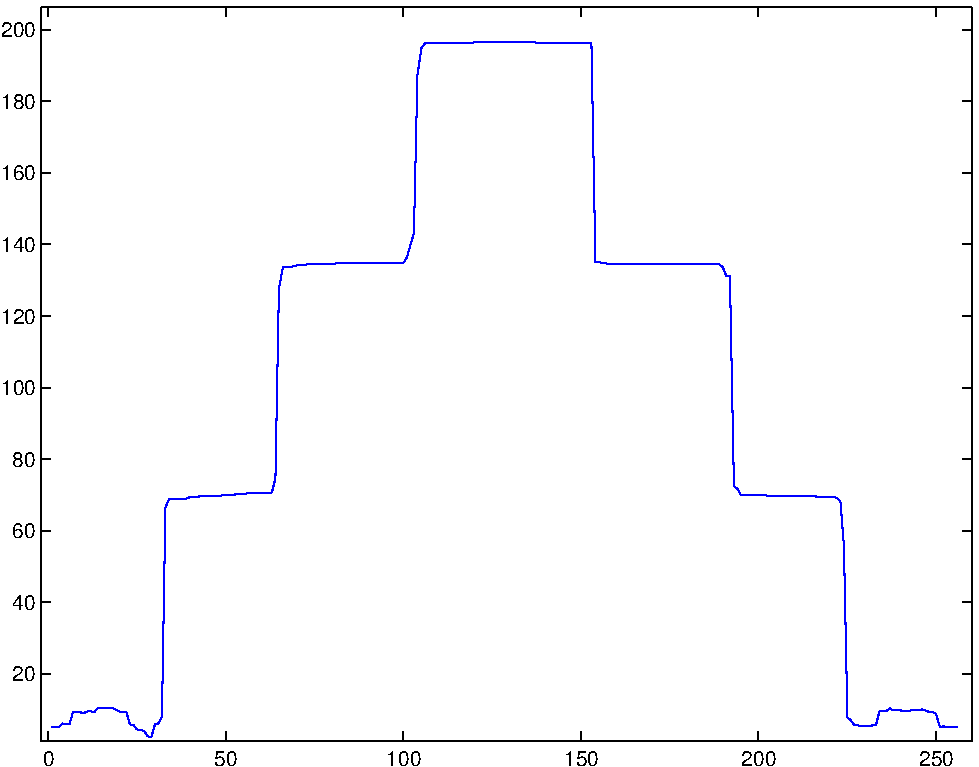
\includegraphics[width=6cm]{img/circles_PID_5_it_93} & 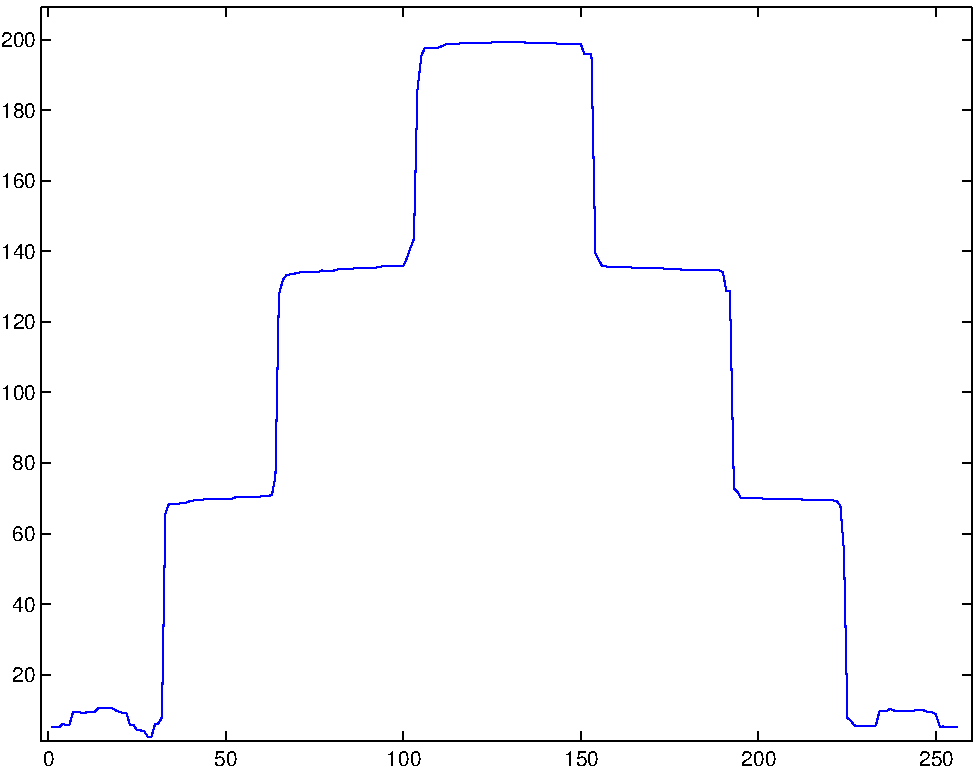
\includegraphics[width=6cm]{img/circles_PID_1_it_92} \\
\\
\mbox{PID5: 93 iterations} & \mbox{PID1: 92 iterations} \\
\\
\\
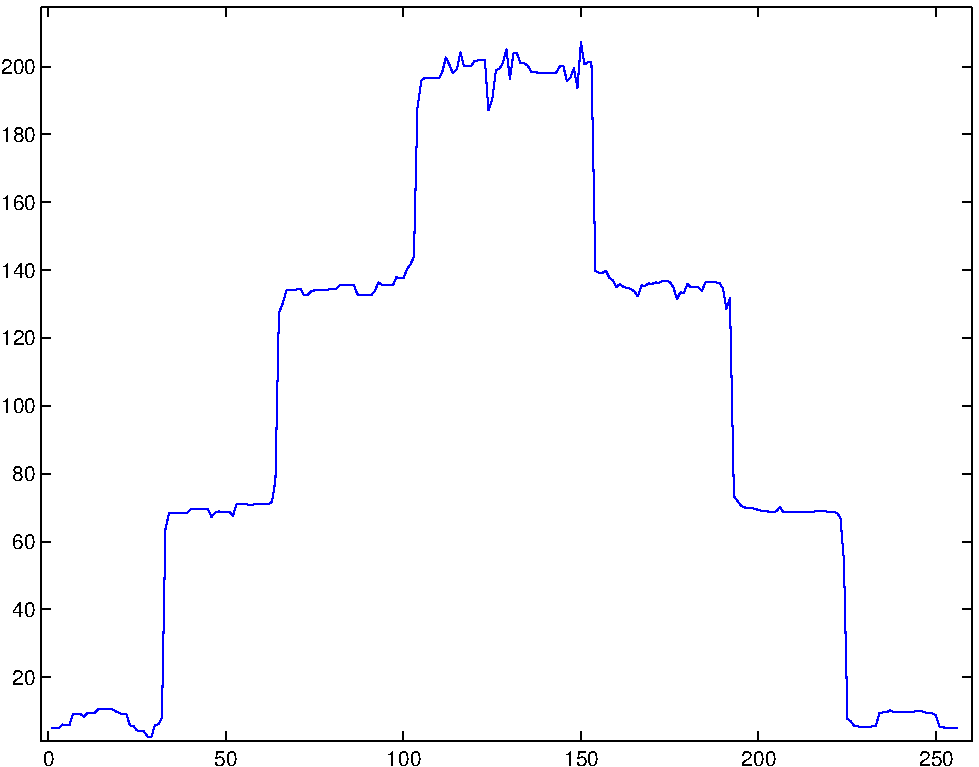
\includegraphics[width=6cm]{img/circles_PID_05_it_88} & \\
\\
\mbox{PID05: 88 iterations} &
\end{array}$
\end{center}
\caption{Line 128 of LCR-1 after 5 seconds}
\end{figure}

%%lcr-10

\begin{figure}[H]
\begin{center}$
\begin{array}{cc}
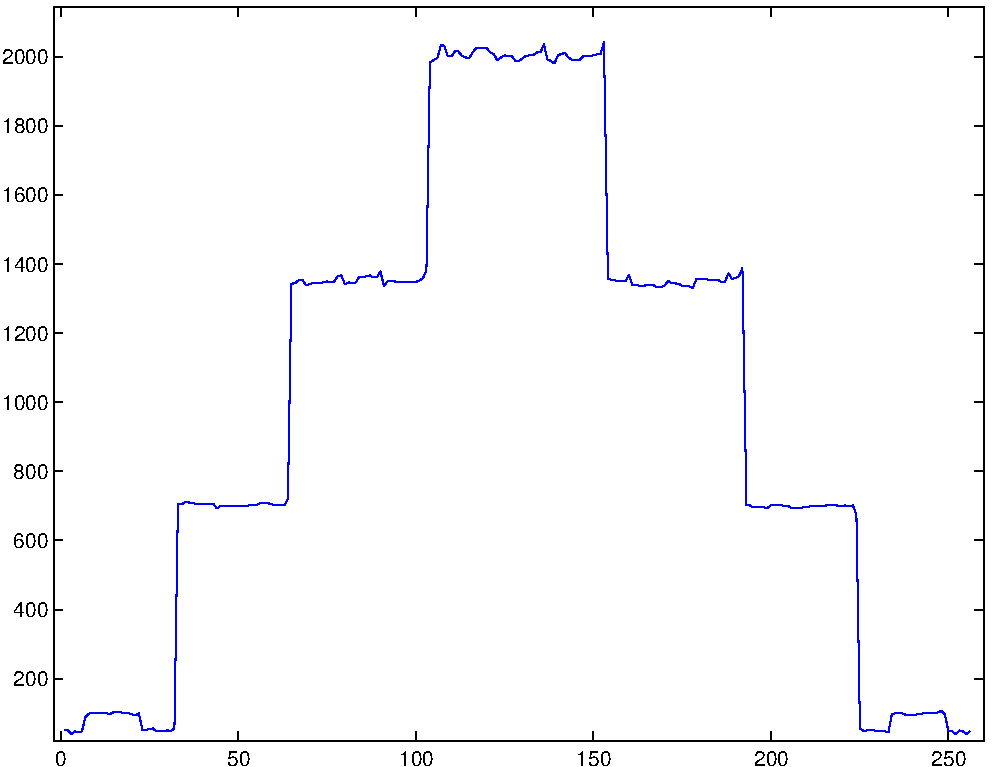
\includegraphics[width=6cm]{img/circles_10_it_99} & 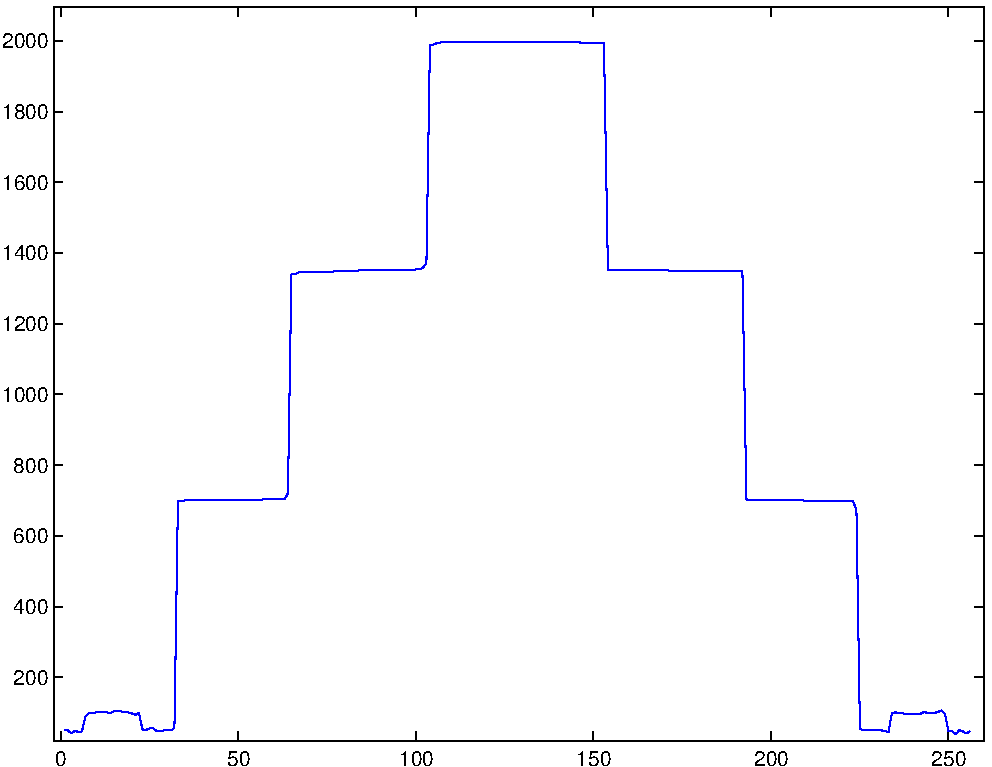
\includegraphics[width=6cm]{img/circles_10_PID_50_it_91} \\
\\
\mbox{AEM: 99 iterations} & \mbox{PID50: 91 iterations} \\
\\
\\
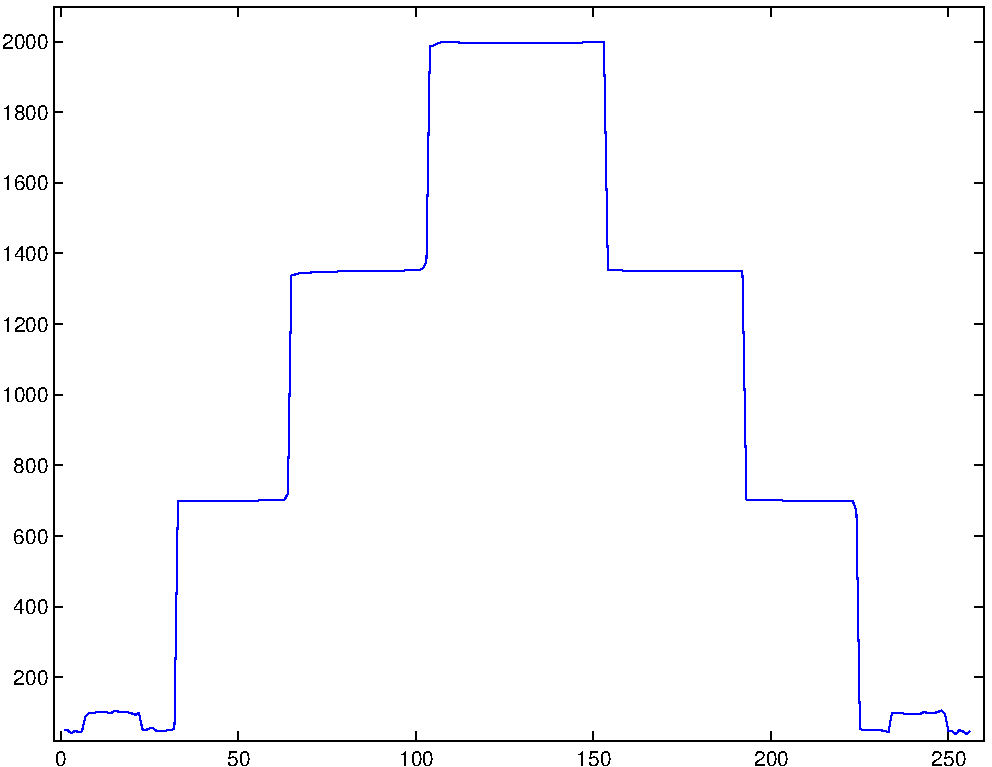
\includegraphics[width=6cm]{img/circles_10_PID_5_it_92} & 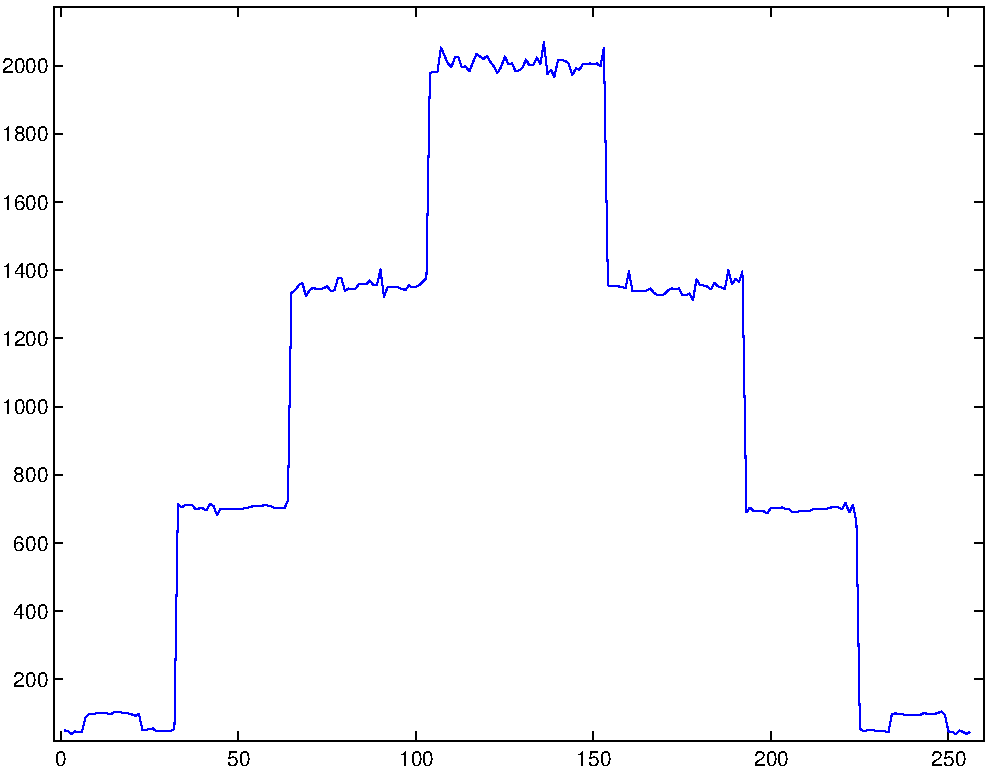
\includegraphics[width=6cm]{img/circles_10_PID_1_it_92} \\
\\
\mbox{PID5: 92 iterations} & \mbox{PID1: 92 iterations} \\
\\
\\
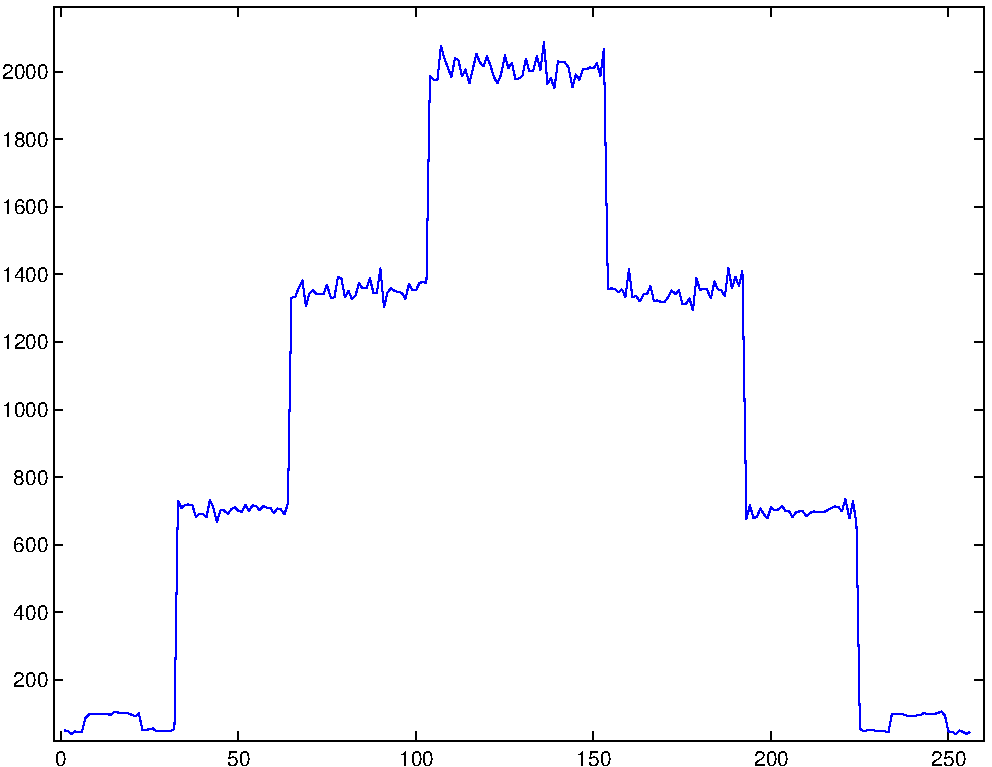
\includegraphics[width=6cm]{img/circles_10_PID_05_it_93} & \\
\\
\mbox{PID05: 93 iterations} &
\end{array}$
\end{center}
\caption{Line 128 of LCR-10 after 5 seconds}
\end{figure}

%% lcr-0.2

\begin{figure}[H]
\begin{center}$
\begin{array}{cc}
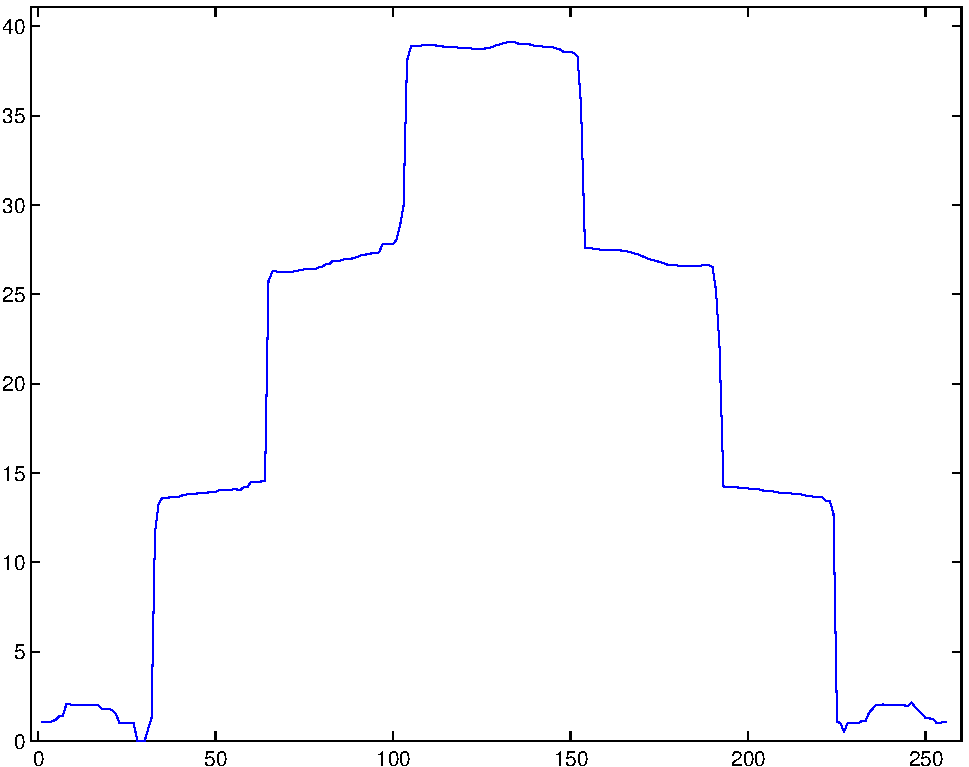
\includegraphics[width=6cm]{img/circles_d5_it_86} & 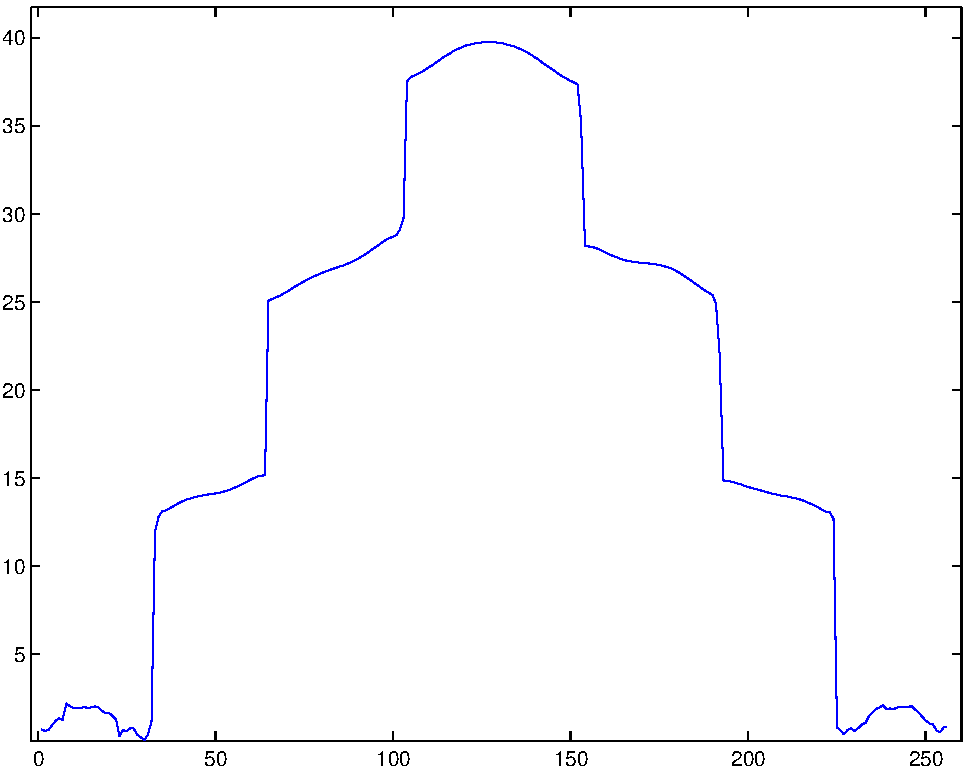
\includegraphics[width=6cm]{img/circles_d5_PID_50_it_98} \\
\\
\mbox{AEM: 86 iterations} & \mbox{PID50: 98 iterations} \\
\\
\\
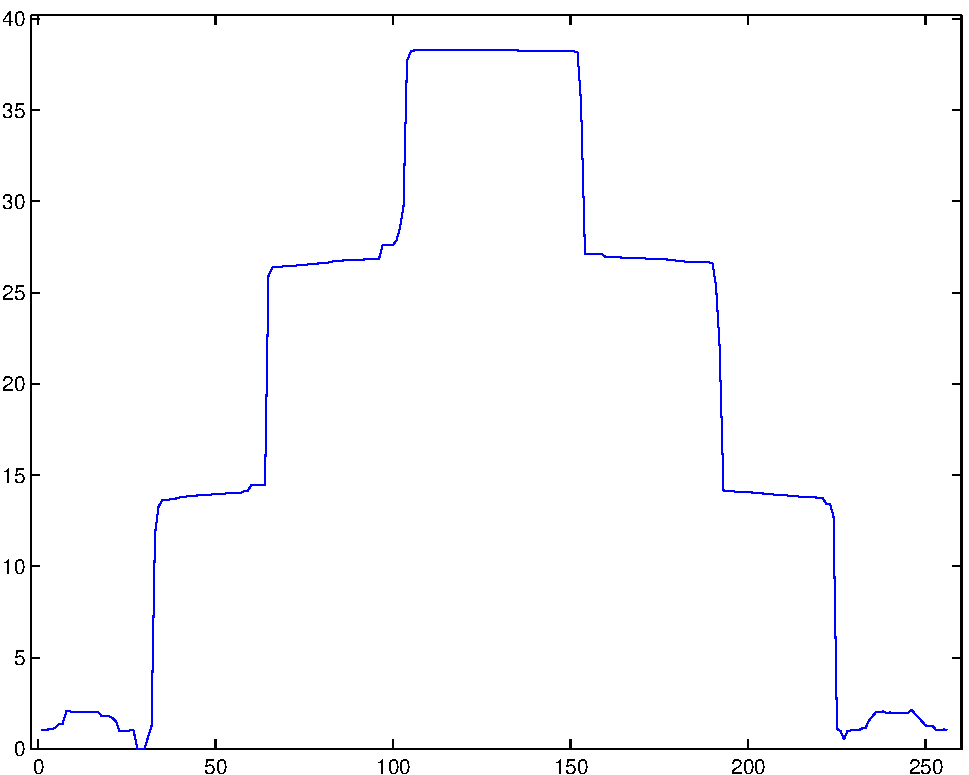
\includegraphics[width=6cm]{img/circles_d5_PID_5_it_97} & 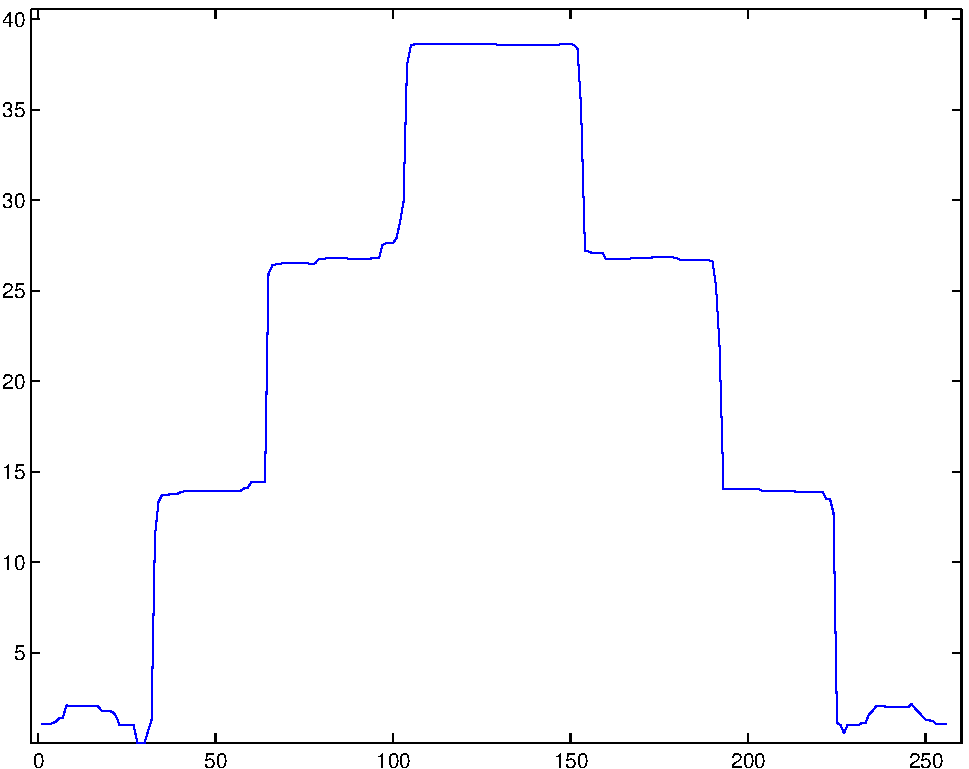
\includegraphics[width=6cm]{img/circles_d5_PID_1_it_91} \\
\\
\mbox{PID5: 97 iterations} & \mbox{PID1: 91 iterations} \\
\\
\\
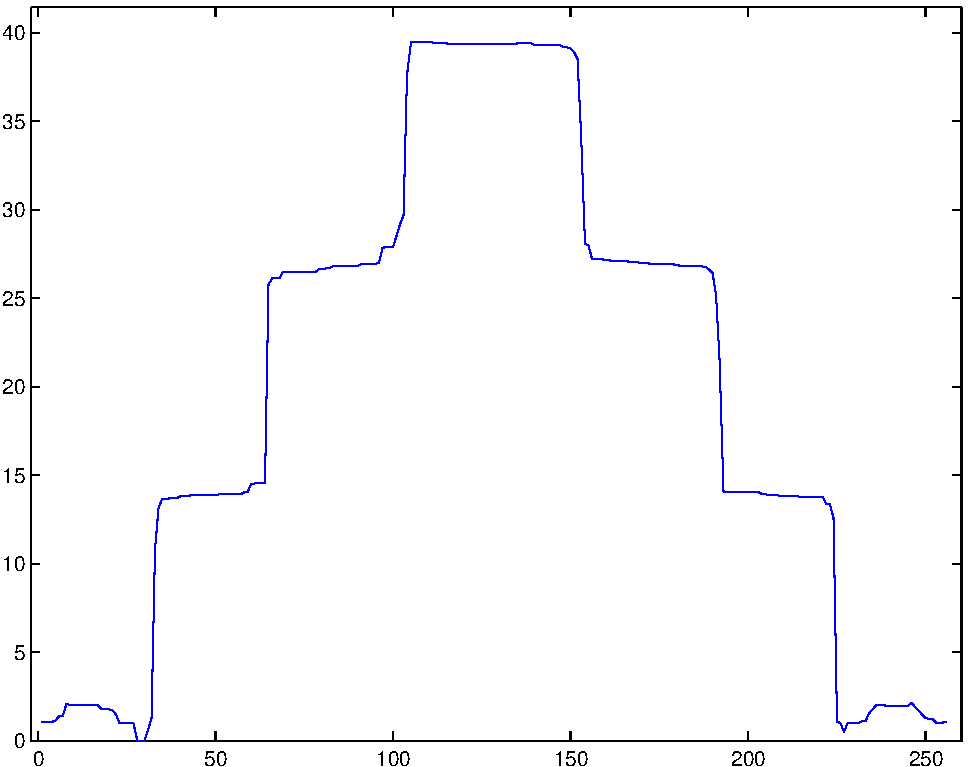
\includegraphics[width=6cm]{img/circles_d5_PID_05_it_93} & \\
\\
\mbox{PID05: 93 iterations} &
\end{array}$
\end{center}
\caption{Line 128 of LCR-0.2 after 5 seconds}
\end{figure}

%% airplane

\begin{figure}[H]
\begin{center}$
\begin{array}{cc}
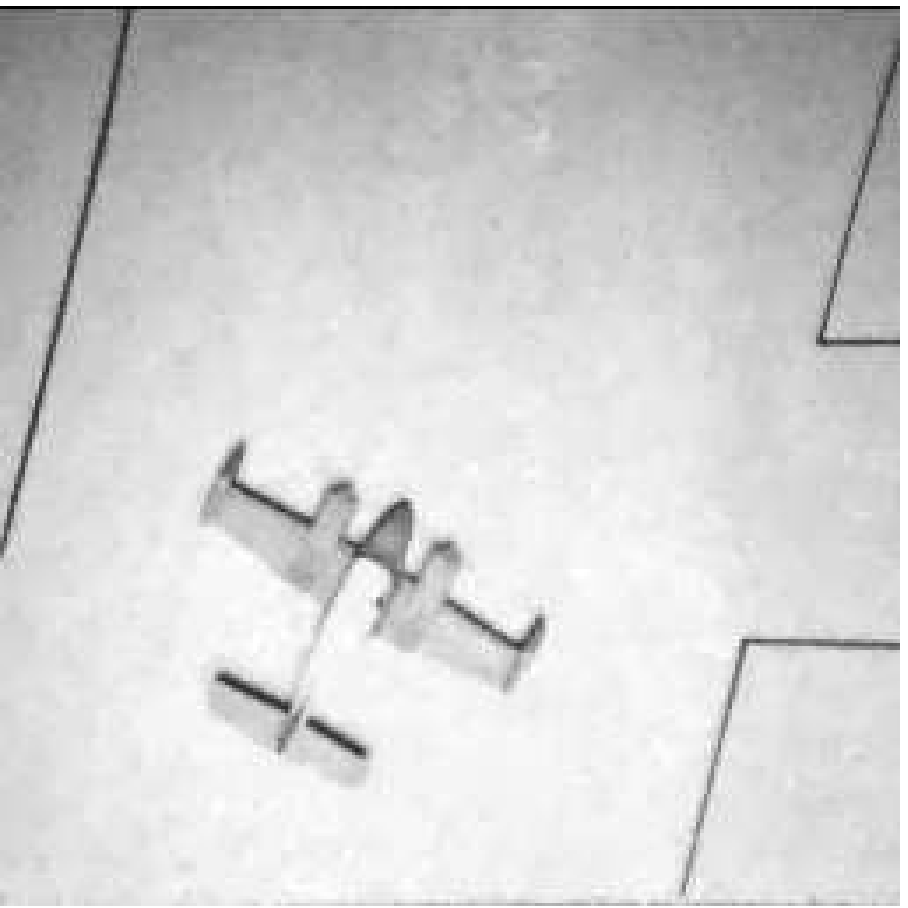
\includegraphics[width=4cm]{img/airplane_it_109} & 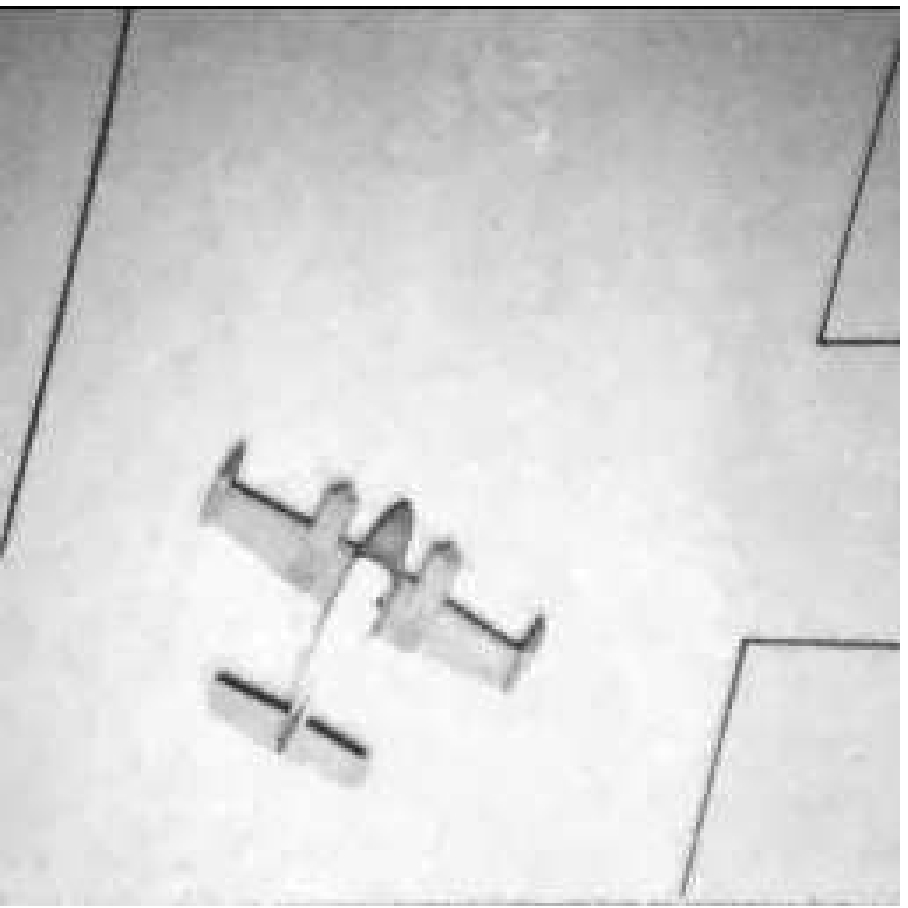
\includegraphics[width=4cm]{img/airplane_PID_50_it_91} \\
\\
\mbox{AEM: 109 iterations} & \mbox{PID50: 91 iterations} \\
\\
\\
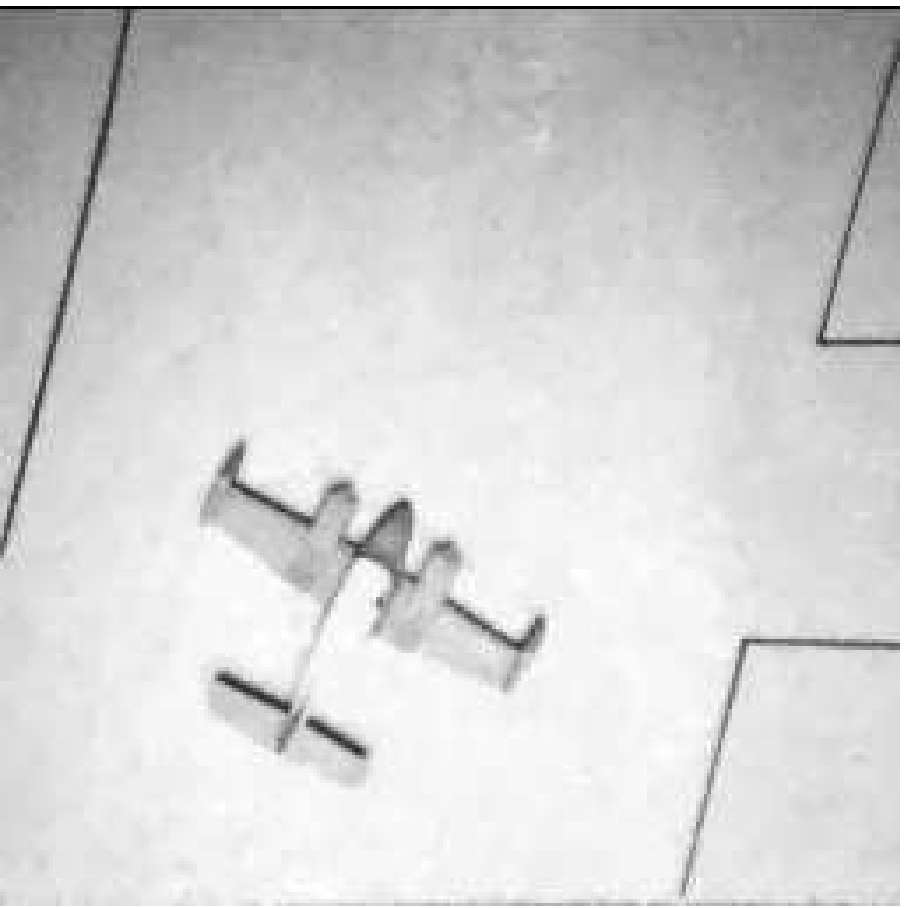
\includegraphics[width=4cm]{img/airplane_PID_5_it_88} & 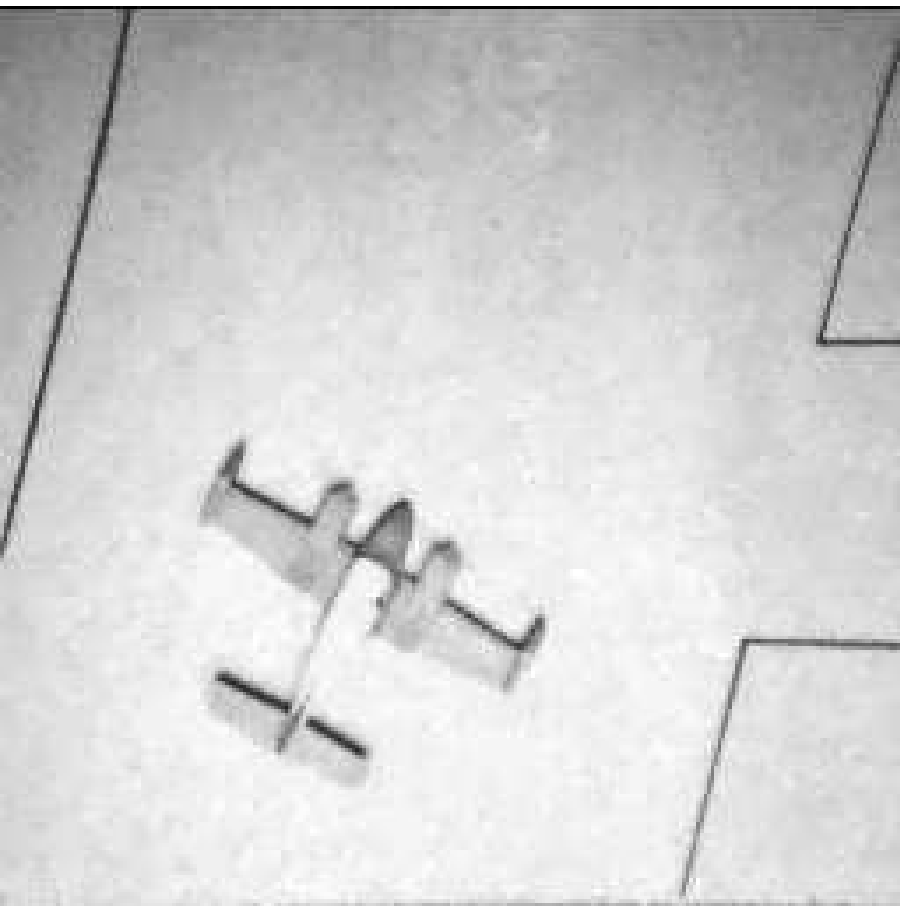
\includegraphics[width=4cm]{img/airplane_PID_1_it_91} \\
\\
\mbox{PID5: 88 iterations} & \mbox{PID1: 91 iterations} \\
\\
\\
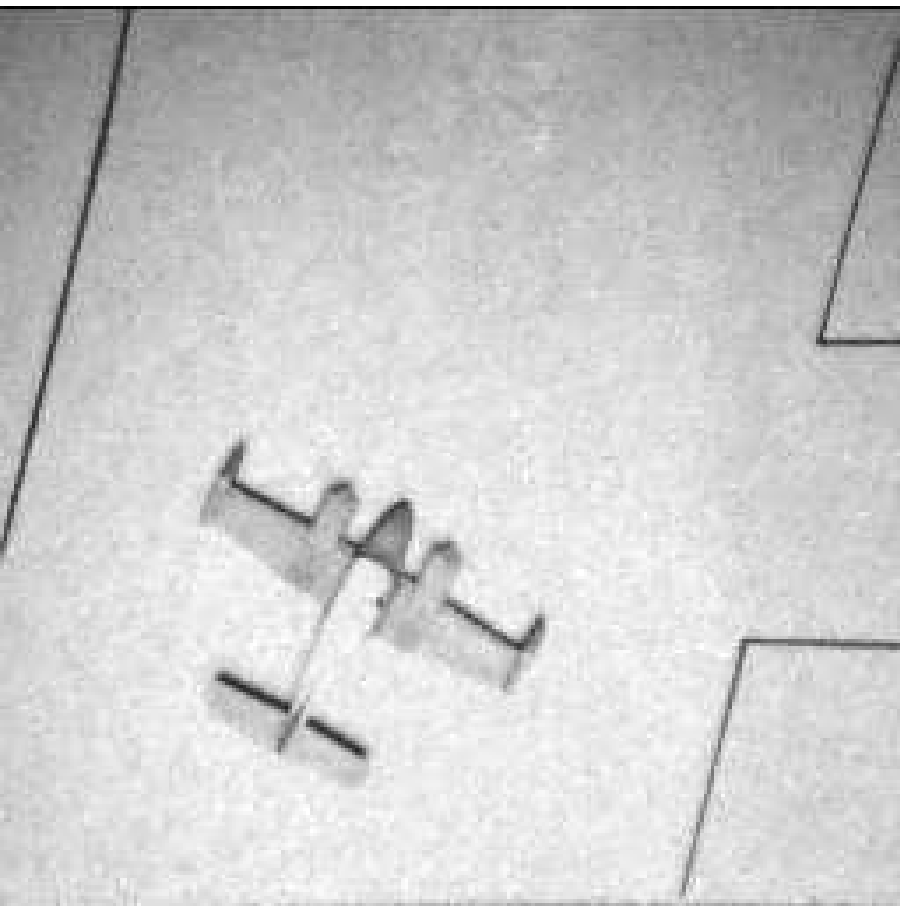
\includegraphics[width=4cm]{img/airplane_PID_05_it_91} & \\
\\
\mbox{PID05: 91 iterations} &
\end{array}$
\end{center}
\caption{Airplane after 5 seconds}
\end{figure}

%% panoramica

\begin{figure}[H]
\begin{center}$
\begin{array}{cc}
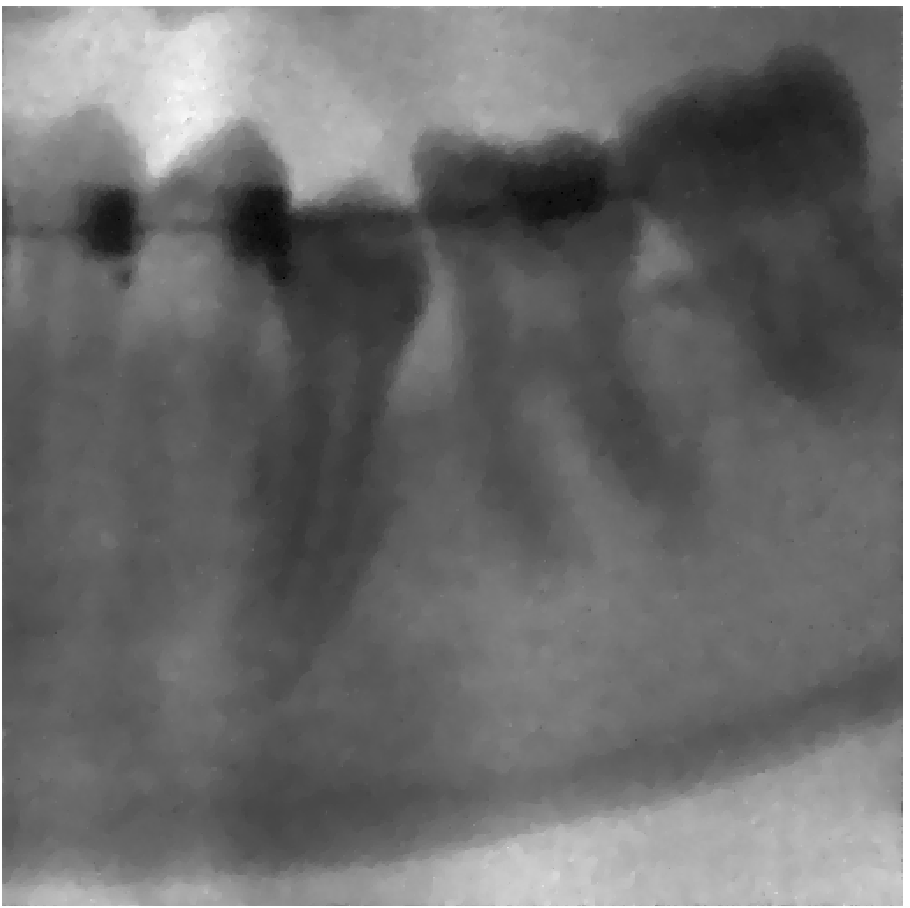
\includegraphics[width=6cm]{img/Panoramica_it_27} & 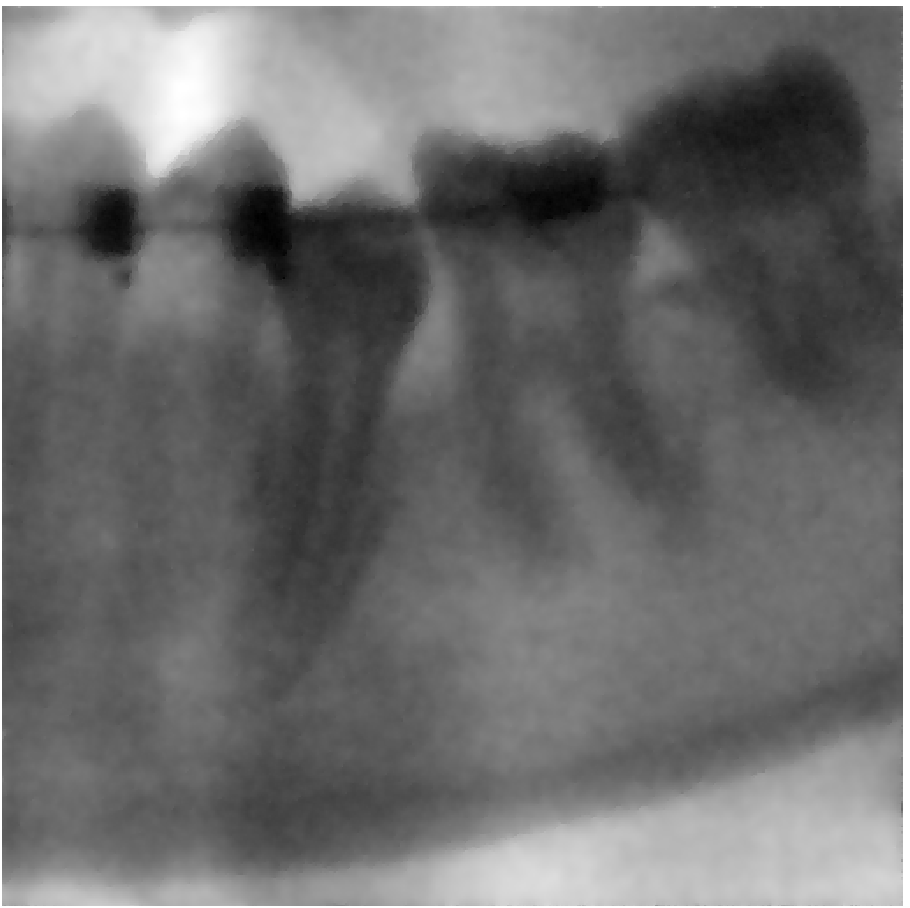
\includegraphics[width=6cm]{img/Panoramica_PID_50_it_27} \\
\mbox{AEM: 27 iterations} & \mbox{PID50: 27 iterations} \\
\\
\includegraphics[width=6cm]{img/Panoramica_PID_5_it_27} & \includegraphics[width=6cm]{img/Panoramica_PID_1_it_24} \\
\mbox{PID5: 27 iterations} & \mbox{PID1: 24 iterations} \\
\\
\includegraphics[width=6cm]{img/Panoramica_PID_05_it_24} & \\
\mbox{PID05: 24 iterations} &
\end{array}$
\end{center}
\caption{DR after 5 seconds}
\end{figure}

From these results we can draw the following remarks.

\begin{itemize}
\item The rate of convergence of PIDSplit+ as a minimization method is strongly conditioned by the choice of the parameter $\gamma$: values which have been observed to give a good initial rate of convergence $\bigl($i.e. high values such as $\frac{50}{\beta}$ and $\frac{5}{\beta}\bigr)$ are not asymptotically satisfactory and \emph{vice versa}.

\item In terms of rates of convergence, AEM is instead located somewhat between the 4 different versions of PIDSplit+, regarding both the initial behavior and the asymptotic one.

\item Any iteration of AEM is, in general, less demanding in terms of computational complexity than any of PIDSplit+, since in the latter the solution of a system is required at each step with the Fast Fourier Transform algorithm (see section \ref{app:circ}).

\item AEM is self-consistent, since it does not depend from any parameter, because the choice of the steplength is adaptive; however, an optimal choice of the parameter $\gamma$ for the PIDSplit+ may provide good results even faster than AEM.

\item If the image considered has a high signal-to-noise ratio (as LCR-0.2) or is significantly bigger than the others (as DR), AEM is observed to have an overall good behavior with respect to the reconstruction error $e^{(rec)}$ also at the initial steps.

\end{itemize}

\section{Behavior of AEM and PIDSplit+ with real-world problems}

In the second set of experiments, considering the images from the project ``PRISMA'', we first compute the optimal value $\beta_{disc}$ for $\beta$, using the discrepancy principle \eqref{discr} proposed in \citep{discr_princ}.

In order to solve the nonlinear equation in $\beta$ involved in the principle, we use a bisection method with the tolerance of $10^{-3}$ combined with AEM to evaluate $x_{\beta}^*$, with the maximum number of iterations set at 3000. The results are the following:

\begin{table}[H]
\begin{center}
\renewcommand*{\arraystretch}{1.6}
\begin{tabular}{|C{1.8cm}|C{2.2cm}|}
\hline
Problem & $\beta_{disc}$ \\
\hline
Image11 & 0.3119 \\ \hline
Image13 & 0.317748 \\ \hline
Image22 & 0.31385 \\ \hline
Image48 & 0.31385 \\ \hline
Image49 & 0.309951 \\ \hline
Image50 & 0.31385 \\
\hline
\end{tabular}
\caption{Values of $\beta_{disc}$ for each image.}
\end{center}
\end{table}

In order to understand the efficacy of such discrepancy principle, we examine some values in the left neighborhood of $\beta_{disc}$, defining as $\beta_{opt}$ the one which provides, among them, the lowest reconstruction error with respect to the ground truth image. Such relative reconstruction error is defined, as previously, as:

$$e^{(iter)} =  \dfrac{||x^{(iter)}-x^*||_2}{||x^*||_2}$$

where $x^*$ is now the ground truth.

The results are shown in the following tables (the line in bold represents the value of $\beta$ chosen as $\beta_{opt}$):

\begin{table}[H]
\begin{center}
\renewcommand*{\arraystretch}{1.6}
\begin{tabular}{|C{1.8cm}|C{1cm}|C{2.2cm}|C{2.2cm}|C{2.2cm}|}
\hline
Problem & $\beta$ & $e^{(3000)}$ & KL & TV \\ \hline
 & 0.01 & 0.0177422 & 2149.67 & 940135 \\ \cline{2-5}
 & \textbf{0.02} & \textbf{0.016393} & \textbf{3915.19} & \textbf{814481} \\ \cline{2-5}
 & 0.05 & 0.0164795 & 7272 & 709033 \\ \cline{2-5}
Image11 & 0.07 & 0.0175498 & 9217.41 & 676261 \\ \cline{2-5}
 & 0.1 & 0.0196065 &  12111.6 & 641869 \\ \cline{2-5}
 & 0.2 & 0.0272481 & 22348.4 & 571412\\ \cline{2-5}
 & 0.3 & 0.0348308 & 34156.3 & 523622\\
\hline
Problem & $\beta$ & $e^{(3000)}$ & KL & TV \\ \hline
 & 0.01 & 0.016544 & 2160.85 & 928899\\ \cline{2-5}
 & \textbf{0.02} & \textbf{0.0152543} & \textbf{3911.13} & \textbf{804136} \\ \cline{2-5}
 & 0.05 & 0.0157587 & 7220.98 & 700156\\ \cline{2-5}
Image13 & 0.07 & 0.0170977 & 9135.89 & 667931\\ \cline{2-5}
 & 0.1 & 0.0194859 & 11991.5 & 633970\\ \cline{2-5}
 & 0.2 & 0.027614 & 21957.3 & 565456\\ \cline{2-5}
 & 0.3 & 0.0353886 & 33566.1 & 518485\\
\hline
Problem & $\beta$ & $e^{(3000)}$ & KL & TV \\ \hline
 & 0.01 & 0.0162132 & 2198.92 & 941487\\ \cline{2-5}
 & \textbf{0.02} & \textbf{0.0148022} & \textbf{4025.25} & \textbf{811476} \\ \cline{2-5}
 & 0.05 & 0.0152197  & 7450.87 & 703634\\ \cline{2-5}
Image22 & 0.07 & 0.0165708 & 9409.18 & 670663\\ \cline{2-5}
 & 0.1 & 0.0190068 & 12318.1 & 636078\\ \cline{2-5}
 & 0.2 & 0.0272591 & 22447.1 & 566297\\ \cline{2-5}
 & 0.3 & 0.0350216 & 34060.9 & 519290\\ \cline{2-5}
\hline
\end{tabular}
\end{center}
\end{table}

\begin{table}[H]
\begin{center}
\renewcommand*{\arraystretch}{1.6}
\begin{tabular}{|C{1.8cm}|C{1cm}|C{2.2cm}|C{2.2cm}|C{2.2cm}|}
\hline
Problem & $\beta$ & $e^{(3000)}$ & KL & TV \\ \hline
 & 0.01 & 0.0154639 & 2157.87 & 932984\\ \cline{2-5}
 & \textbf{0.02} & \textbf{0.0139999} & \textbf{3917.88} & \textbf{807767} \\ \cline{2-5}
 & 0.05 & 0.0144383 & 7249.03 & 703296\\ \cline{2-5}
Image48 & 0.07 & 0.0157969 & 9165.57 & 671017\\ \cline{2-5}
 & 0.1 & 0.0182356 & 12013.4 & 637173\\ \cline{2-5}
 & 0.2 & 0.0267319 & 22221.7 & 566942\\ \cline{2-5}
 & 0.3 & 0.0346593 & 33915.8 & 519601\\
\hline
Problem & $\beta$ & $e^{(3000)}$ & KL & TV \\ \hline
 & 0.01 & 0.0160722 & 2159.3 & 940036\\ \cline{2-5}
 & \textbf{0.02} & \textbf{0.0145997} & \textbf{3949.21} & \textbf{812753} \\ \cline{2-5}
 & 0.05 & 0.148771 & 7346.71 & 706008\\ \cline{2-5}
Image49 & 0.07 & 0.0161719 & 9307.99 & 672987\\ \cline{2-5}
 & 0.1 & 0.0185724 & 12237.8 & 638159\\ \cline{2-5}
 & 0.2 & 0.0268924 & 22499.1 & 567536\\ \cline{2-5}
 & 0.3 & 0.0348179 & 34338.2 & 519626\\
\hline
Problem & $\beta$ & $e^{(3000)}$ & KL & TV \\ \hline
 & 0.01 & 0.0158575 & 2175.75 & 932012\\ \cline{2-5}
 & \textbf{0.02} & \textbf{0.0144898} & \textbf{3963.06} & \textbf{804892} \\ \cline{2-5}
 & 0.05 & 0.0150870 & 7921.30 & 699159\\ \cline{2-5}
Image50 & 0.07 & 0.0165020 & 9225.63 & 667082\\ \cline{2-5}
 & 0.1 & 0.0902397 & 12087.30 & 633079\\ \cline{2-5}
 & 0.2 & 0.0276045 & 22290.52 & 562893\\ \cline{2-5}
 & 0.3 & 0.0355275 & 33892.61 & 515937\\
\hline
\end{tabular}
\end{center}
\end{table}


Using both $\beta_{opt}$ and $\beta_{disc}$ we run AEM and PIDSplit+ for all of the images considered, setting a maximum number of 3000 iterations and using the following stopping criterion:

\begin{align}
\label{stopping}
\dfrac{||w^{(k+1)}-w^{(k)}||_2}{||w^{(k+1)}||_2} < 10^{-6}
\end{align}

where, for AEM:

$$w^{(k)} = \left( x^{(k)} , y^{(k)} \right)^T$$

while, for PIDSplit+:

$$w^{(k)} = \left( x^{(k)} , w_1^{(k)} , w_2^{(k)} , w_3^{(k)} , b_1^{(k)} , b_2^{(k)} , b_3^{(k)} \right)^T$$

In the following tables we show the time elapsed for each run of the algorithm considered, along with the number of iterations performed before satisfying the stopping criterion, the relative reconstruction error obtained and the value of the primal function.

The $^*$ mark indicates that the stopping criterion has not been fulfilled and the algorithm stopped due to the maximum number of iterations reached.

\begin{table}[H]
\begin{center}
\renewcommand*{\arraystretch}{1.5}
\begin{tabular}{|C{1.2cm}|C{1cm}|C{1cm}|C{1.8cm}|C{1.8cm}|}
\hline
Method & $t^{(iter)}$ & \emph{iter} & $e^{(iter)}$ & $\phi\left(x^{(iter)}\right) $  \\ \hline
& \multicolumn{4}{c|} {$\beta_{opt}$} \\ \hline
 AEM & 11.93 & 242 & 0.0163191 & 19931.5    \\ \hline
 PID50 & 69.68 & 793 & 0.0163193 & 19931.6  \\ \hline
 PID5 & 8.77 & 101 & 0.0163191 & 19931.6   \\ \hline
 PID1 & 25.67 & 295 & 0.0163184 & 19931.6   \\ \hline
 PID05 & 42.75 & 486 & 0.0163183 & 19331.7   \\ \hline
 & \multicolumn{4}{c|} {$\beta_{disc}$} \\ \hline
%% & $t^{(iter)}$ & \emph{iter} & $e^{(iter)} $ & $f^{(iter)}$ \\ \hline
AEM &   140.05 & 2616 & 0.356273 & 194203\\ \hline
PID50  &  78.41 & 906 & 0.035957 & 194200 \\ \hline
PID5 &   56.73 & 651 & 0.0358966 & 194198\\ \hline
PID1 &   191.92 & 2228 & 0.0355936 & 194204\\ \hline
PID05 &   $258.6^*$ & $3000^*$ & $0.0345798^*$  & $194273^*$ \\ \hline
\end{tabular}
\end{center}
\caption{Results for Image11.}
\end{table}

% im 13

\begin{table}[H]
\begin{center}
\renewcommand*{\arraystretch}{1.5}
\begin{tabular}{|C{1.2cm}|C{1cm}|C{1cm}|C{1.8cm}|C{1.8cm}|}
\hline
 Method & $t^{(iter)}$ & \emph{iter} & $e^{(iter)}$ & $\phi\left(x^{(iter)}\right) $ \\ \hline
& \multicolumn{4}{c|} {$\beta_{opt}$}  \\ \hline
AEM & 12.74 & 241 & 0.0152054 & 19735.4  \\ \hline
PID50 &  70.85 & 819 & 0.015209 & 19735.4 \\ \hline
PID5 & 8.82 &103& 0.0152087& 19735.4 \\ \hline
PID1 & 25.9 & 294 & 0.0152068 & 19735.4 \\ \hline
PID05 & 41.75 &483& 0.015205 &19735.6 \\ \hline
& \multicolumn{4}{c|} {$\beta_{disc}$} \\ \hline
AEM & 133.62 & 2648 & 0.0365654 & 195065 \\ \hline
PID50 & 79.05 & 910 & 0.0369184 &195062 \\ \hline
PID5 & 55.79 & 655 & 0.0368513 & 195060  \\ \hline
PID1 & 195.75 & 22.48 & 0.0365267 & 195066 \\ \hline
PID05 & $260.33^*$ & $3000^*$ & $0.354137^*$ & $195142^*$ \\ \hline
\end{tabular}
\end{center}
\caption{Results for Image13.}
\end{table}

%im22

\begin{table}[H]
\begin{center}
\renewcommand*{\arraystretch}{1.5}
\begin{tabular}{|C{1.2cm}|C{1cm}|C{1cm}|C{1.8cm}|C{1.8cm}|}
\hline
 Method & $t^{(iter)}$ & \emph{iter} & $e^{(iter)}$ & $\phi\left(x^{(iter)}\right) $ \\ \hline
 & \multicolumn{4}{c|} {$\beta_{opt}$}  \\ \hline
AEM & 12.45 & 241 & 0.0147852 & 19966 \\ \hline
PID50 & 73.4 & 843 & 0.0147872 & 19966.1 \\ \hline
PID5 & 9.15 & 105 & 0.0147871 & 19966.1 \\ \hline
PID1 & 25.98 & 297 & 0.0147855 & 19966 \\ \hline
PID05 & 43.06 & 488 & 0.0147841 & 19966.2 \\ \hline
& \multicolumn{4}{c|} {$\beta_{disc}$} \\ \hline
AEM & 134.51 & 2628 & 0.0359532 & 193683 \\ \hline
PID50 & 79.08 & 909 & 0.0362905 & 193680 \\ \hline
PID5 & 56.64 & 651 & 0.0362275 & 193678 \\ \hline
PID1 & 190.93 & 2234 & 0.0359172 & 193684 \\ \hline
PID05 & $258.15^*$ & $3000^*$ & $0.0348683^*$ & $193755^*$ \\ \hline
\end{tabular}
\end{center}
\caption{Results for Image22.}
\end{table}

% im 48

\begin{table}[H]
\begin{center}
\renewcommand*{\arraystretch}{1.5}
\begin{tabular}{|C{1.2cm}|C{1cm}|C{1cm}|C{1.8cm}|C{1.8cm}|}
\hline
 Method & $t^{(iter)}$ & \emph{iter} & $e^{(iter)}$ & $\phi\left(x^{(iter)}\right) $ \\ \hline
 & \multicolumn{4}{c|} {$\beta_{opt}$}  \\ \hline
AEM & 13.71 & 242 & 0.0139344 & 19793.2 \\ \hline
PID50 & 77.43 & 887 & 0.013936 & 19793.3 \\ \hline
PID5 & 9.69 & 110 & 0.0139358 & 19793.3 \\ \hline
PID1 & 26.21 & 302 & 0.0139345 & 19793.2\\ \hline
PID05 & 43.13 & 495 & 0.013934 & 19793.4 \\ \hline
& \multicolumn{4}{c|} {$\beta_{disc}$} \\ \hline
AEM & 140.12 & 2623 & 0.0356696 & 193509 \\ \hline
PID50 & 79.23 & 928 & 0.0360122 & 193506 \\ \hline
PID5 & 56.87 & 651 & 0.0359488 & 193504 \\ \hline
PID1 & 195.64 & 2234 & 0.0356353 & 193510 \\ \hline
PID05 & $259.99^*$ & $3000^*$ & $0.0345653^*$ & $193582^*$ \\ \hline
\end{tabular}
\end{center}
\caption{Results for Image48.}
\end{table}

% im 49

\begin{table}[H]
\begin{center}
\renewcommand*{\arraystretch}{1.5}
\begin{tabular}{|C{1.2cm}|C{1cm}|C{1cm}|C{1.8cm}|C{1.8cm}|}
\hline
 Method & $t^{(iter)}$ & \emph{iter} & $e^{(iter)}$ & $\phi\left(x^{(iter)}\right) $ \\ \hline
 & \multicolumn{4}{c|} {$\beta_{opt}$}  \\ \hline
AEM & 12.77 & 243 & 0.014611 & 19908.6  \\ \hline
PID50 & 73.32 & 841 & 0.0146128 & 19908.6  \\ \hline
PID5 & 9.27 & 106 & 0.0146125 & 19908.6  \\ \hline
PID1 & 26.21 & 302 & 0.0146112 & 19908.6  \\ \hline
PID05 & 43.59 & 496 & 0.0146104 & 19908.8  \\ \hline
& \multicolumn{4}{c|} {$\beta_{disc}$} \\ \hline
AEM & 130.64 & 2594 & 0.0355119 & 191946  \\ \hline
PID50 & 79.4 & 921 & 0.0358461 & 191943  \\ \hline
PID5 & 55.04 & 645 & 0.035784 & 191941  \\ \hline
PID1 & 192.5 & 2205 & 0.035474 & 191947  \\ \hline
PID05 & $259.79^*$ & $3000^*$ & $0.0344835^*$ & $192011^*$  \\ \hline
\end{tabular}
\end{center}
\caption{Results for Image49.}
\end{table}

% im 50

\begin{table}[H]
\begin{center}
\renewcommand*{\arraystretch}{1.5}
\begin{tabular}{|C{1.2cm}|C{1cm}|C{1cm}|C{1.8cm}|C{1.8cm}|}
\hline
 Method & $t^{(iter)}$ & \emph{iter} & $e^{(iter)}$ & $\phi\left(x^{(iter)}\right) $ \\ \hline
 & \multicolumn{4}{c|} {$\beta_{opt}$}  \\ \hline
AEM & 11.88 & 242 & 0.0145248 & 19762.3 \\ \hline
PID50 & 73.02 & 837 & 0.014528 & 19762.4 \\ \hline
PID5 & 9.5 & 105 & 0.0145277 & 19762.4 \\ \hline
PID1 & 26.03 & 300 & 0.0145258 & 19762.3 \\ \hline
PID05 & 43.01 & 494 & 0.0145241 & 19762.5 \\ \hline
& \multicolumn{4}{c|} {$\beta_{disc}$} \\ \hline
AEM & 132.21 & 2619 & 0.0365043 & 192324 \\ \hline
PID50 & 81.43 & 951 & 0.036849 & 192321 \\ \hline
PID5 & 55.45 & 647 & 0.0367837 & 192319 \\ \hline
PID1 & 195.34 & 2223 & 0.0394668 & 192324 \\ \hline
PID05 & $261.35^*$ & $3000^*$ & $0.0354126^*$ & $192394^*$ \\ \hline
\end{tabular}
\end{center}
\caption{Results for Image50.}
\end{table}

Below are shown the images resulting from PIDSplit+ with $\gamma = \dfrac{5}{\beta}$ for both $\beta_{opt}$ and $\beta_{disc}$.

\begin{figure}[H]
\begin{center}$
\begin{array}{cc}
\includegraphics[width=6cm]{img/Image11_PID_5_002.pdf}  & \includegraphics[width=6cm]{img/Image11_PID_5_03119.pdf}
\\
\beta_{opt} & \beta_{disc}
\end{array}$
\end{center}
\caption{Image11 after the stopping criterion has been reached.}
\end{figure}

\begin{figure}[H]
\begin{center}$
\begin{array}{cc}
\includegraphics[width=6cm]{img/Image13_PID_5_002.pdf}  & \includegraphics[width=6cm]{img/Image13_PID_5_031775.pdf}
\\
\beta_{opt} & \beta_{disc}
\end{array}$
\end{center}
\caption{Image13 after the stopping criterion has been reached.}
\end{figure}

\begin{figure}[H]
\begin{center}$
\begin{array}{cc}
\includegraphics[width=6cm]{img/Image22_PID_5_002.pdf}  & \includegraphics[width=6cm]{img/Image22_PID_5_031385.pdf}
\\
\beta_{opt} & \beta_{disc}
\end{array}$
\end{center}
\caption{Image22 after the stopping criterion has been reached.}
\end{figure}

\begin{figure}[H]
\begin{center}$
\begin{array}{cc}
\includegraphics[width=6cm]{img/Image48_PID_5_002.pdf}  & \includegraphics[width=6cm]{img/Image48_PID_5_031385.pdf}
\\
\beta_{opt} & \beta_{disc}
\end{array}$
\end{center}
\caption{Image48 after the stopping criterion has been reached.}
\end{figure}

\begin{figure}[H]
\begin{center}$
\begin{array}{cc}
\includegraphics[width=6cm]{img/Image49_PID_5_002.pdf}  & \includegraphics[width=6cm]{img/Image49_PID_5_030995.pdf}
\\
\beta_{opt} & \beta_{disc}
\end{array}$
\end{center}
\caption{Image49 after the stopping criterion has been reached.}
\end{figure}

\begin{figure}[H]
\begin{center}$
\begin{array}{cc}
\includegraphics[width=6cm]{img/Image50_PID_5_002.pdf}  & \includegraphics[width=6cm]{img/Image50_PID_5_031385.pdf}
\\
\beta_{opt} & \beta_{disc}
\end{array}$
\end{center}
\caption{Image50 after the stopping criterion has been reached.}
\end{figure}

Below, instead,  are shown the images resulting from the PIDSplit+ with the optimal value of $\gamma$ (always $\frac{5}{\beta}$, as can be seen from the previous tables) and AEM, for $\beta = \beta_{opt}$:

\begin{figure}[H]
\begin{center}$
\begin{array}{cc}
\includegraphics[width=6cm]{img/Image11_PID_5_002.pdf}  & \includegraphics[width=6cm]{img/Image11_002.pdf}
\\
\mbox{PID5} & \mbox{AEM}
\end{array}$
\end{center}
\caption{Image11 after the stopping criterion has been reached.}
\end{figure}

\begin{figure}[H]
\begin{center}$
\begin{array}{cc}
\includegraphics[width=6cm]{img/Image13_PID_5_002.pdf}  & \includegraphics[width=6cm]{img/Image13_002.pdf}
\\
\mbox{PID5} & \mbox{AEM}
\end{array}$
\end{center}
\caption{Image13 after the stopping criterion has been reached.}
\end{figure}

\begin{figure}[H]
\begin{center}$
\begin{array}{cc}
\includegraphics[width=6cm]{img/Image22_PID_5_002.pdf}  & \includegraphics[width=6cm]{img/Image22_002.pdf}
\\
\mbox{PID5} & \mbox{AEM}
\end{array}$
\end{center}
\caption{Image22 after the stopping criterion has been reached.}
\end{figure}

\begin{figure}[H]
\begin{center}$
\begin{array}{cc}
\includegraphics[width=6cm]{img/Image48_PID_5_002.pdf}  & \includegraphics[width=6cm]{img/Image48_002.pdf}
\\
\mbox{PID5} & \mbox{AEM}
\end{array}$
\end{center}
\caption{Image48 after the stopping criterion has been reached.}
\end{figure}

\begin{figure}[H]
\begin{center}$
\begin{array}{cc}
\includegraphics[width=6cm]{img/Image49_PID_5_002.pdf}  & \includegraphics[width=6cm]{img/Image49_002.pdf}
\\
\mbox{PID5} & \mbox{AEM}
\end{array}$
\end{center}
\caption{Image49 after the stopping criterion has been reached.}
\end{figure}

\begin{figure}[H]
\begin{center}$
\begin{array}{cc}
\includegraphics[width=6cm]{img/Image50_PID_5_002.pdf}  & \includegraphics[width=6cm]{img/Image50_002.pdf}
\\
\mbox{PID5} & \mbox{AEM}
\end{array}$
\end{center}
\caption{Image50 after the stopping criterion has been reached.}
\end{figure}

From the results of these experiments we can draw the following remarks.

\begin{itemize}
\item The stopping criterion \eqref{stopping} used for both the algorithms provides good results, considering also that the values of the primal function $f\left(x^{(k)}\right)$ using both AEM and PIDSplit+ (with the optimal value for $\gamma$), are comparable.

\item From the results obtained with $\beta_{opt}$ and $\beta_{disc}$, indipendently from the image considered, it can bee seen that the reconstruction obtained using $\beta_{disc}$ seems to be excessively smoothed, with the loss of many details of the original image. For this reason, the adoption of such value for $\beta$ seems advisable if the result required is to distinguish between different areas of the image. It appears that $\beta_{disc}$ provide an overestimation for the order of magnitude of $\beta$.

\item As seen before, the values of $\gamma$ affects heavily the behavior of the PIDSplit+ algorithm, to the point that the stopping criterion \eqref{stopping} is sometimes not satisfied within the maximum number of iterations.

\item As previously, an optimal choice for the user-supplied parameter $\gamma$ provides good results even with the considered stopping criterion; in general AEM has a less efficient behavior than the optimal PIDSplit+, although with fairly similar values.
\end{itemize} 
\appendix
\chapter{}

\section{Notable matrix structures} \label{app:matrices}

\subsection{Toepliz matrices}
\label{sec:matrices}

A \emph{Toepliz matrix}, named after the mathematician Otto Toepliz, is a matrix in which each descending diagonal from left to right is costant, as in the following example:

$$
\begin{pmatrix}
a & b & c & d & e \\
f & a & b & c & d \\
g & f & a & b & c \\
h & g & f & a & b \\
i & h & g & f & a \\
\end{pmatrix}
$$

More generally, as a $n \times n$ matrix, a Toepliz matrix has the form:

$$T = \begin{pmatrix}
a_0 & a_{-1} & a_{-2} & \cdots & \cdots & a_{-n+1} \\
a_1 & a_0 & a_{-1} & \ddots & \ddots & a_{-n+2} \\
a_2 & a_1 & a_0 & \ddots & \ddots &\vdots \\
\vdots & \ddots & \ddots & \ddots & a_{-1} & a_{-2} \\
\vdots & \ddots & \ddots & a_1 & a_0 & a_{-1} \\
a_{n-1} & \cdots & \cdots & a_2 & a_1 & a_0
\end{pmatrix}
$$

$T$ is uniquely determined by their diagonals, thus one could consider their position with respect to the main diagonal and name the elements

$$a_i \left\{ \begin{array}{ll}
i=0 &\qquad \mbox{ the main diagonal} \\
i=1 &\qquad \mbox{ the first diagonal below}\\
i=-1&\qquad \mbox{ the first diagonal above} \\
\vdots & \qquad \qquad \vdots
\end{array} \right.$$

In a block-Toepliz matrix each element is a matrix as well; if such element is a Toepliz matrix, we have a block-Toepliz with Toepliz blocks matrix (BTTB).

An interesting properties of Toepliz matrices is that the convolution operation can be constructed as a matrix multiplication, where one of the inputs is converted into a Toeplitz matrix.

\subsection{Fourier matrices}

A Fourier matrix, which represent the Fourier transform, is a matrix of order $n$

$$F_n = \dfrac{1}{\sqrt{n}}\begin{pmatrix}
1 & 1 & 1 & \dots & 1 \\
1 & w & w^2 & \dots & w^{n-1} \\
1 & w^2 & w^4 & \dots & w^{2(n-1)} \\
\vdots & \vdots & \vdots & \ddots & \vdots \\
1 & w^{n-1} & w^{2(n-1)} & \dots & w^{(n-1)(n-1)}
\end{pmatrix}$$

where $w$ is a $n$-th root of 1:

$$ w= e^{-i \frac{2\pi}{n}} = \cos \left(\dfrac{2\pi}{n} \right) - i \sin \left( \dfrac{2\pi}{n} \right)$$

and $i$ is the imaginary unit.

Since $w^k$, $k=0,1,...$ is periodic with period $n$, $F_n$ is reduced to:

$$F_n = \dfrac{1}{\sqrt{n}}\begin{pmatrix}
1 & 1 & 1 & \dots & 1 \\
1 & w & w^2 & \dots & w^{n-1} \\
1 & w^2 & w^4 & \dots & w^{n-2} \\
\vdots & \vdots & \vdots & \ddots & \vdots \\
1 & w^{n-1} & w^{n-2} & \dots & w
\end{pmatrix}$$


A \emph{discrete Fourier transform} (DFT), denoted by $\mathcal{F}$, of a vector $f \in \R^n$ is the matrix-vector product

$$\mathcal{F}(f) = F_n f$$

Fourier matrices has interesting properties: if we denote the matrix conjugate traspose of $F_n$ with $F_n^*$, we have $F_n^* = \overline{F_n}^T$,

$F_n$ and $F_n^*$ are symmetric and $F_n$ is unitary, i.e.

$$F_n^* F_n = F_n F_n^* = I \qquad \mbox{ or } \qquad F_n^{-1} = F_n^*$$

The DFT of a vector of $n$ entries can be computed using a \emph{fast Fourier transform} (FFT) algorithm with complexity $O(n \log_2 n)$ and similarly for the inverse FFT.

The Fourier transform of a 2-D $n \times n$ image $f(x,y)$ can then be expressed using the Kroenecker product of $F_n$:

$$(F_n \otimes F_n) vec(f)$$

where $vec(f)$ is an array of $n^2$ entries column-wise ordered.

If we consider the $n$ matrix form of the image, we can show that

$$mat \biggl( \left(F_n \otimes F_n\right) vec(f)\biggr) = F_n f F_n^T = F_n f F_n$$

\subsection{Circulant matrices} \label{app:circ}

A circulant matrix  $n\times n$ is a particular Toepliz matrix of the form

$$C = \begin{pmatrix}
c_0 & c_{n-1} & \dots & c_2 & c_1 \\
c_1 & c_0 & c_{n-1} & \dots & c_2 \\
\vdots & \ddots & \ddots & \ddots & \vdots \\
c_{n-2} & \ddots & c_1 & c_0 & c_{n-1} \\
c_{n-1} & c_{n-2} & \dots & c_1 & c_0 \\
\end{pmatrix}
$$

$C$ is then completely determined by its first column

$$c=(c_0,c_1,\dots, c_{n-1})^T$$

If the elements of this matrix are matrices as well, we have a block-circulant matrix, if such matrices are circulant, we have a block-circulant with circulant blocks matrix (BCCB).

Any Circulant matrix $C$ can be diagonalized by the Fourier matrix \citep{circulant}:

$$C = F_n^* \Lambda F_n $$

where $F_n$ is the Fourier matrix of order $n$, $\Lambda$ is the diagonal matrix of the eigenvalues of $C$ and $F_n^*$ are the corresponding eigenvectors.

We observe that

$$F_n C = \Lambda F_n$$

and if we consider only the first column of the matrix equality, we have

$$F_n c = \dfrac{1}{\sqrt{n}} (\lambda_1,...,\lambda_n)^T$$

since the first column of $F_n$ has all entries equal to $\dfrac{1}{\sqrt{n}}$.

Then $diag{\Lambda} =  \sqrt{n} \mathcal{F}(c)$

Similarly, in a Block Circulant matrix, each block is decomposed using the Fourier matrix $F_n$: $C_k = F_n^* \Lambda_k F_n$, where $\Lambda_k$ is the diagonal matrix of the eigenvalues of each block $C_k$.

If we have a BCCB matrix $\mathbf{C}$, it is diagonalized\citep{circulant}:

$$\mathbf{C} = (F_n \otimes F_n)^* \Lambda (F_n \otimes F_n)$$

where

$$\Lambda = \sum_{k=0}^{n-1} (\Omega_n^k \otimes \Lambda_k) \qquad \mbox{ and } \qquad \Omega_n = diag(1,w,w^2,...,w^{n-1})$$

This relationship between circulant matrices and Fourier matrices is very useful: if we consider $Cx=b$, where $C$ is circulant, we can write such equation as $c * x = b$, where $c$ is, as previously, the first column of $C$, $*$ denotes the convolution operator, and both $x$ and $b$ are cyclically extended in each direction.

Using the result of the circular convolution theorem, we can trasform the cyclic convolution into component-wise multiplication using the DFT:

$$\mathcal{F}(c * x) = \mathcal{F}(c) \mathcal{F}(x) = \mathcal{F}(b)$$

Then we have

$$x = \mathcal{F}^{-1} \left(\dfrac{\mathcal{F}(b)}{\mathcal{F}(c)}\right)$$

If we use the FFT algorithm, such equation is a very efficient way to compute $x$.
If we have to compute the matrix product vector $Cx$ we have

$$\mathcal{F}^{-1} (\mathcal{F}(c) \cdot \mathcal{F}(x) ) = b $$

\section{Constrained optimization}

A general constrained optimization problem can be expressed as:

\begin{align}
\label{min}
\minimize_{x \in \R^n} f(x) \qquad \mbox{subject to} \; \left\{ \begin{array}{l}
c_i(x) = 0 \\
c_j(x) \geq 0 \\
\end{array} \right. \qquad
\end{align}

where $c_i(x)$ and $c_j(x)$ (with $i \in \mathcal{E}, j \in \mathcal{I}$) are vectorial functions at least $C^2$, called, respectively, the \emph{equality constraints} and \emph{inequality constraints}. $f$ is called the \emph{objective function}.

Furthermore, we define the \emph{feasible set} $\Omega$ to be the set of points $x$ that satisfy the constraints, that is

$$\Omega = \{ x | h_i (x) = 0 \;,\; g_i(x) \geq 0\}$$

With this notation \eqref{min} can be written more compactly as

$$\minimize_{x \in \Omega} f(x) $$

The solution of \eqref{min} is a point of \emph{local minimum}, defined more rigorously as

\begin{defi}
A point $x^* \in \R^n$  is a point of local minimum if $x^* \in \Omega$ and exists a neighborhood $U$ of $x^*$ such that $f(x) \geq f(x^*) \; \forall x \in U \cap \Omega$.
\end{defi}

\subsection{First order necessary conditions}

In order to give the first order necessary conditions, a couple of definitions and an assumption, the \emph{constraint qualification}, is required, to foresee any degenerate behaviour of the function.

\begin{defi}
The \emph{Lagrangian} function for the constrained optimization problem \eqref{min} is:

$$\mathcal{L}(x,\lambda) = f(x) - \sum_{i \in \mathcal{E} \cup I} \lambda_i c_i (x)$$
\end{defi}

\begin{defi}
The \emph{active set} $A(x)$ at any feasible point $x$ is the set

$$\mathcal{A}(x^*) = \mathcal{E} \cup \{ i \in \mathcal{I} | c_i(x^*) = 0\}$$
\end{defi}

\begin{defi}
Given the point $x^*$, we say that the \emph{linear indipendence constraint qualifications} (LICQ) holds if the set of active constraint gradient $\{ \nabla c_i (x^*)| i \in \mathcal{A}(x^*)\}$ is linearly independent.
\end{defi}

This condition allows the statement of the following optimality conditions for a general nonlinear programming problem as in \eqref{min}. They are called the first-order conditions because they concern the properties of the gradients of the objective and constraint functions.

\begin{theorem}[First-order necessary condition]

Suppose that $x^*$ is a local solution of \eqref{min} and that LICQ holds at $x^*$. Then there is a Lagrange multiplier vector $\lambda^*$ with components $\lambda_i^*$ ($i \in \mathcal{E}\cup \mathcal{I}$) such that the following conditions are satisfied at $(x^*,\lambda^*)$:

\begin{align}
\label{KKT}
\begin{aligned}
\nabla_x \mathcal{L}(x^*,\lambda^*) &= 0  && \\
\\
c_i (x^*) &= 0 && \forall i \in \mathcal{E} \\
\\
c_i (x^*) &\geq 0 && \forall i \in \mathcal{I} \\
\\
\lambda_i^* &\geq 0 && \forall i \in \mathcal{I} \\
\\
\lambda_i^* c_i (x^*) &= 0 && \forall i \in \mathcal{E} \cup \mathcal{I}
\end{aligned}
\end{align}
\begin{proof}
See \citep{nocedal} p. 331.
\end{proof}
\end{theorem}

The conditions expressed in this theorem are often known as the \emph{Karush-Kuhn-Tucker conditions} (KKT).

\subsection{Second order necessary and sufficient conditions}

\begin{defi}
Given a point $x^*$ and the active constraint set $\mathcal{A}(x^*)$, the set $F_1$  is defined by:

$$F_1 = \left\{ \alpha d \left| \begin{array}{ll}
d^T \nabla c_i(x^*) = 0 & \forall i \in \mathcal{E} \\
\\
d^T \nabla c_i(x^*) \geq 0 & \forall i \in \mathcal{I} \end{array} \right. \right\} $$
\end{defi}

Such set $F_1$ is a cone, and when a constraint qualification as LICQ is satisfied, it represent the \emph{tangent cone} to the feasible set at $x^*$.

\begin{defi}
Given $F_1$ and the Lagrange multiplier vector $\lambda^*$ satisfying the KKT conditions \eqref{KKT}, we define the subset $F_2(\lambda^*)$ of $F_1$ by:

$$ F_2 (\lambda^*) = \left\{ w \in F_1 \left| w^T \nabla c_i(x^*) = 0 \right. \qquad \forall i \in \mathcal{A}(x^*) \cap \mathcal{I} \; \mbox{ with }\; \lambda_i^* > 0 \right\} $$
\end{defi}

Such subset $F_2(\lambda^*)$ contains the directions $w$ that tend to ``adhere'' to the active inequality constraints for which the Lagrange multiplier component $\lambda_i^* > 0$, as well as to the equality constraints. This set is important because contains directions from $F_1$ for which it is not clear from first derivative information alone whether $f$ will increase or decrease.

Then, the necessary condition involving the second derivatives is described by the following theorem:

\begin{theorem}[Second-order necessary condition]
Suppose that $x^*$ is a local solution of \eqref{min} and that LICQ condition is satisfied. Let $\lambda^*$ be a Lagrange multiplier vector such that the KKT conditions \eqref{KKT} are satisfied and let $F_2(\lambda^*)$ be defined as above.

Then

$$ w^T \nabla_{xx} \mathcal{L}(x^*,\lambda^*) w \geq 0 \qquad \forall w \in F_2(\lambda^*)$$

\begin{proof}
See \citep{nocedal}, p. 343.
\end{proof}
\end{theorem}

The second-order sufficient condition looks very much like the necessary conditions just stated, but it differs in that the constraint qualification is not required and the inequality is replaced by a strict inequality.

\begin{theorem}[Second-order sufficient condition]
Suppose that for some feasible point $x^* \in \R^n$ there is a Lagrange multiplier vector $\lambda^*$ such that KKT conditions \eqref{KKT} are satisfied.

Suppose also that

$$ w^T \nabla_{xx} \mathcal{L}(x^*,\lambda^*) w > 0 \qquad \forall w \in F_2(\lambda^*), w \neq 0$$

Then $x^*$ is a strict local solution for \eqref{min}.

\begin{proof}
See \citep{nocedal}, p. 345.
\end{proof}
\end{theorem}

\subsection{Convex optimization} \label{app:convex}

\begin{defi}
A function $f: S \to \R $ is convex if $\forall x_1,x_2 \in S$ we have that

$$f\Bigl((1-\rho)x_1+\rho x_2\Bigr) \leq (1-\rho)f(x_1)+\rho f(x_2)$$

with $\rho \in (0,1)$.

\end{defi}

Convex functions are very important in numerical optimization, as shows the following theorem:

\begin{theorem}
A convex problem satisfies one of the following:

\begin{itemize}
\item there is not a solution to the minimum problem
\item every local solution is a global solution
\end{itemize}

\begin{proof}

By \emph{reductio ad absurdum} suppose that exists a local solution $x^*$ which is not a global solution, that is

$$\exists z \; \mbox{ such that } \; f(z ) \leq f(x^*)$$

$f$ is convex:

$$f\Bigl((1-\rho) x^* + \rho z \Bigr) \leq (1-\rho)f(x^*) + \rho f(z) = f(x^*) + \rho(f(z)-f(x^*)) $$

Note that this last term $\rho\Bigl(f(z)-f(x^*)\Bigr) \leq 0$ since $ \rho \neq 0$.

If $x = x^* + \rho (z-x^*) = (1 -\rho) x^* + \rho z$, we have that

$$f(x) \leq f(x^*) \Rightarrow \nexists \delta > 0 \; \mbox{ such that }\; f(x) \geq f(x^*)$$

that means $x^*$ is not a local solution, which contradicts our supposition.
\end{proof}
\end{theorem}

In order to ensure the existence of a global minimum, we require the function to be coercive:

\begin{defi}
A function $f: \R^n \to \R^n$ is \emph{coercive} if

$$\lim_{||x|| \to \infty} f(x) = + \infty$$
\end{defi}

Convex functions have other interesting properties:

\begin{theorem} \label{app:monotone}
Let $f: R^n \to R^n$ be a convex function.

Then $\nabla f(x)$ is a monotone function.

\begin{proof}

Since $f(x)$ is convex, we have that

\begin{align*}
f(x) &\geq f(y) + \nabla f(y)^T (x-y) \\
f(y) &\geq f(x) + \nabla f(x)^T (y-x) \\
\end{align*}

Adding the two equations, we have:

$$(\nabla f(y) - \nabla f(x))^T (y-x) \geq 0$$
\end{proof}
\end{theorem}

\begin{theorem}
Let $f(x,y)$ be convex with respect to $x$ and concave with respect to $y$.

Then

$$\begin{pmatrix} \nabla_x f(x,y) \\
\\
-\nabla_y f(x,y) \end{pmatrix}$$

is monotone.

\begin{proof}

Since

\begin{align*}
f(x_i,y_i) &\geq f(x_i',y_i) + \nabla_x f(x_i',y_i) (x_i - x_i') \\
f(x_i,y_i) &\geq f(x_i,y_i') + \nabla_y f(x_i,y_i') (y_i - y_i') \\
\end{align*}

we have that

\begin{align*}
(\nabla_x &f(x_1,y_1) - \nabla_x f(x_2,y_2))^T (x_1-x_2) + (\nabla_y f(x_1,y_2) + \\
&- \nabla_y f(x_2,y_1))^T (y_1-y_2) \geq 0
\end{align*}
\end{proof}
\end{theorem}

\chapter{Matlab scripts}

In this chapter we will provide the MATLAB scripts used throughout this thesis, in alphabetical order:

\section{AEM.m}
\lstinputlisting{src/AEM.m}

\section{app.m}
\lstinputlisting{src/app.m}

\section{beta\_array.m}
\lstinputlisting{src/beta_array.m}

\section{beta\_bisez.m}
\lstinputlisting{src/beta_bisez.m}

\section{iter\_AEM.m}
\lstinputlisting{src/iter_AEM.m}

\section{iter\_PID.m}
\lstinputlisting{src/iter_PID.m}

\section{PIDSplit\_plus.m}
\lstinputlisting{src/PIDSplit_plus.m}

\section{prisma.m}
\lstinputlisting{src/prisma.m}



\bibliography{biblio}
\bibliographystyle{unsrt}
\end{document} 